\documentclass[master=cws,masteroption=gs,english]{kulemt/kulemt}
\setup{title={A Middleware For Secure And Protected Data Aggregation},
  author={Jesse Geens},
  promotor={Prof.\,dr.\,ir.\ W. Joosen \and dr. B. Lagaisse \and Prof. dr. V. Naessens},
  assessor={Ir.\,W. Eetveel\and W. Eetrest},
  assistant={E. H. Beni \and A. Rafique}}
% De volgende \setup mag verwijderd worden als geen fiche gewenst is.
\setup{filingcard,
  translatedtitle={Een middleware voor veilige en beveiligde dataverzameling},
  udc=621.3,
  shortabstract={Hier komt een heel bondig abstract van hooguit 500
    woorden. \LaTeX\ commando's mogen hier gebruikt worden. Blanco lijnen
    (of het commando \texttt{\string\pa r}) zijn wel niet toegelaten!
    \endgraf \lipsum[2]}}
% Verwijder de "%" op de volgende lijn als je de kaft wil afdrukken
%\setup{coverpageonly}
% Verwijder de "%" op de volgende lijn als je enkel de eerste pagina's wil
% afdrukken en de rest bv. via Word aanmaken.
%\setup{frontpagesonly}

% Kies de fonts voor de gewone tekst, bv. Latin Modern
\setup{font=lm}

%% TODO come up with name and insert it here
\newcommand{\middleware}{(middleware)}

% PassOptionsToPackage fixes line breaks in URLs
\PassOptionsToPackage{hyphens}{url}\usepackage[pdfusetitle,colorlinks,plainpages=false]{hyperref}
\hypersetup{%
  citecolor=blue!70,
  linkcolor=black,
}

\usepackage{float}

% for formal definitions
\usepackage{framed}

% environment derived from framed.sty: see leftbar environment definition
\newenvironment{formal}{%
  \def\FrameCommand{%
    \definecolor{formalshade}{rgb}{0.95,0.95,1}
    \definecolor{darkblue}{rgb}{0.0, 0.0, 0.55}
    \hspace{1pt}%
    {\color{darkblue}\vrule width 2pt}%
    {\color{formalshade}\vrule width 4pt}%
    \colorbox{formalshade}%
  }%
  \MakeFramed{\advance\hsize-\width\FrameRestore}%
  \noindent\hspace{-4.55pt}% disable indenting first paragraph
  \begin{adjustwidth}{}{7pt}%
  \vspace{2pt}\vspace{2pt}%
}
{%
  \vspace{2pt}\end{adjustwidth}\endMakeFramed%
}

% cite (author, year) style
\usepackage{natbib}
%\bibliographystyle{abbrvnat}
\bibliographystyle{unsrtnat}
\setcitestyle{authoryear,open={(},close={)}}

%%%%%%%
% Om wat tekst te genereren wordt hier het lipsum pakket gebruikt.
% Bij een echte masterproef heb je dit natuurlijk nooit nodig!
\IfFileExists{lipsum.sty}%
 {\usepackage{lipsum}\SetLipsumDefault{11-13}}%
 {\newcommand{\lipsum}[1][11-13]{\par Hier komt wat tekst: lipsum ##1.\par}}
%%%%%%%

% Set todos in text
\usepackage{todonotes}

% For diagrams
\usepackage{rotating}
\usepackage{pdflscape}
\usepackage[sort]{cleveref}
\usetikzlibrary{arrows}

%%%%%%%
% Custom code listings
\usepackage{listings}
\usepackage{color}
\usepackage{chngcntr}

% Enumerations with letters instead of numbers
\usepackage{enumitem}

% Acronyms
\usepackage[acronym,smallcaps]{glossaries}

\loadglsentries{acronyms}
\makeglossaries
\glsdisablehyper

% Default fixed font does not support bold face
\DeclareFixedFont{\ttb}{T1}{txtt}{bx}{n}{12} % for bold
\DeclareFixedFont{\ttm}{T1}{txtt}{m}{n}{12}  % for normal

% Language support for turtle
\definecolor{deepblue}{rgb}{0,0,0.5}
\definecolor{deepred}{rgb}{0.6,0,0}
\definecolor{deepgreen}{rgb}{0,0.5,0}
\definecolor{antiquewhite}{rgb}{0.98, 0.92, 0.84}

\lstdefinestyle{turtle}{
    %backgroundcolor = \color{antiquewhite},
    basicstyle=\footnotesize,
    numbers=left,
    stepnumber=1,
    % morecomment=[l]{\# },
    %% TODO fix only comment if hashtag followed by space
    keywordstyle=\footnotesize\color{deepblue},
    emph={Authorization, agentClass, Agent, mode, Read, Write, Control, accessTo, agent},
    morekeywords={acl, @prefix, foaf},             % Add keywords here
    %keywordstyle=\color{green},
    commentstyle=\itshape\color{orange},
    %emphstyle=\footnotesize\color{deepred},    % Custom highlighting style
     emphstyle={\color{deepgreen}},
    stringstyle=\color{deepgreen},
    frame=t,                         % Any extra options here
    showstringspaces=false,
}

% Language support for JSON
\colorlet{punct}{red!60!black}
\definecolor{background}{HTML}{EEEEEE}
\definecolor{delim}{RGB}{20,105,176}
\colorlet{numb}{magenta!60!black}

\lstdefinelanguage{json}{
    basicstyle=\normalfont\ttfamily,
    numbers=left,
    numberstyle=\scriptsize,
    stepnumber=1,
    numbersep=8pt,
    showstringspaces=false,
    breaklines=true,
    frame=lines,
    %backgroundcolor=\color{background},
    literate=
     *{0}{{{\color{numb}0}}}{1}
      {1}{{{\color{numb}1}}}{1}
      {2}{{{\color{numb}2}}}{1}
      {3}{{{\color{numb}3}}}{1}
      {4}{{{\color{numb}4}}}{1}
      {5}{{{\color{numb}5}}}{1}
      {6}{{{\color{numb}6}}}{1}
      {7}{{{\color{numb}7}}}{1}
      {8}{{{\color{numb}8}}}{1}
      {9}{{{\color{numb}9}}}{1}
      {:}{{{\color{punct}{:}}}}{1}
      {,}{{{\color{punct}{,}}}}{1}
      {\{}{{{\color{delim}{\{}}}}{1}
      {\}}{{{\color{delim}{\}}}}}{1}
      {[}{{{\color{delim}{[}}}}{1}
      {]}{{{\color{delim}{]}}}}{1},
}

%%%%%%%%%
% Fix quotes, see https://tex.stackexchange.com/questions/356898/quote-with-author-reference-at-the-end
\let\oldquote\quote
\let\endoldquote\endquote
\renewenvironment{quote}[2][]
  {\if\relax\detokenize{#1}\relax
     \def\quoteauthor{#2}%
   \else
     \def\quoteauthor{#2~---~#1}%
   \fi
   \oldquote}
  {\par\nobreak\smallskip\hfill(\quoteauthor)%
   \endoldquote\addvspace{\bigskipamount}}

% No horizontal table overflows
\usepackage{tabulary}

%\includeonly{chap-n}
\begin{document}

% Make listing numbers follow chapters
\counterwithin{lstlisting}{chapter}

\begin{preface}
\begin{fancyquote}{\textit{Sir Tim Berners-Lee}}
``I found myself answering the same questions asked frequently of me by different people. It would be so much easier if everyone could just read my database.''
\end{fancyquote}

\noindent Solid is an amazing technology that has the potential to change the web as we know it. The last year, I have witnessed amazing progress being made in this domain, and I am truly honored that I had the opportunity to be a part of it. It has been quite the roller coaster, combining my dissertation research with a semester spent abroad on an Erasmus exchange, but it was well worth the effort. There are an endless amount of people I want to thank for supporting me through this period, especially my friends and family.\\

\noindent First and foremost, my most sincere gratitude goes to my girlfriend Elise, who had to endure endless streams of complaints when I was stuck somewhere, and screams of joy when I made some progress. Without her support, this text would not be the same.\\

\noindent Secondly, I owe an immense amount of gratitude to my supervisors and assistant-supervisors. 
In particular, I want to thank Bert Lagaisse for allowing me to combine my dissertation while studying in Hungary, which was not a trivial task. Your feedback and guidance taught me a lot and greatly improved the quality of my work. I also want to thank Emad and Kristof for the great advice and encouragement every week. Your advice has inspired me many times and your kind words have always encouraged me. Finally, I also want to explicitly thank prof. Vincent Naessens, prof. Wouter Joosen and Dimitri Van Landuyt for their valuable feedback and suggestions.\\

\noindent Thirdly, I want to thank my family for supporting me not only through this dissertation, but throughout my whole study career. I owe a large part of my successes to their support. I especially want to thank my father and grandfather for inspiring me to study a technical domain, and for teaching me to always think critically.\\

\noindent Lastly, I want to thank my father and my friends Benjamin, Aram and Tobias for proofreading and improving this text. 

\end{preface}

\tableofcontents*

\begin{abstract}
  In recent years, the internet has become evermore centralized \citep{internet-report}. This has many negative side effects, such as decreased competition and a lack of access to personal data \citep{big-tech-innovation, platform-monopolies}. Solid \citep{solid} is a new draft W3C specification that aims to combat this by introducing pods. Pods are decentralized datastores where user data is kept for many different applications. In this manner, the user retains control over his personal data, and the same data can be used across different services.
  
  These pods provide a number of possibilities, but also come with technological challenges. One such challenge is secure and protected data aggregation across different pods. Such data aggregations impose privacy risks, as well as scalability issues. This dissertation presents a server-level middleware that aims to partially resolve these issues by presenting two novel technologies: privacy filters, and a new token mechanism that supports decentralized delegation.
  
  Privacy filters is a technology that enables more granularity in the privacy of shared resources. When a request is made, the middleware selects a number of transformations to perform on the requested resource, based on the user's settings and contextual parameters such as the requesting application and the resource's data type. To subsequently attain a token mechanism that supports decentralized delegation, this dissertation investigates the use of macaroons as a token mechanism in Solid. Macaroons not only provide decentralized token delegation, but are also much more efficient to generate and verify. Moreover, they allow third-party attestations, which is a useful property for realizing pods belonging to a group of agents.
  
  The middleware presented in this dissertation has been evaluated on the basis of three use cases. For privacy filters, a number of performance experiments have demonstrated that the overhead of the middleware is tolerable for smaller resources. Rewriting resources of around 300KB using three transformations causes an overhead of around 50\% in the request duration. However, larger resources (around 3MB) have overheads that become a five-fold of the original request duration. As such, a more efficient method for resource rewriting may be necessary here, although this issue can be lessened by making use of caching and precomputation. Performance experiments on the generation and verification of macaroons have illustrated that macaroons offer large performance benefits. The throughput of generating and verifying macaroons is seven and eleven times higher respectively, compared to \acrshort{DPoP} using the ES256 algorithm. Finally, there are also theoretical gains for decentralized delegation in a reduced number of needed interactions for realizing token delegation.
\end{abstract}

\begin{abstract*}
  De afgelopen jaren is het internet steeds meer gecentraliseerd geworden \citep{internet-report}. Dit heeft vele negatieve gevolgen, waaronder gedaalde concurrentie en een gebrek aan toegang tot persoonlijke gegevens \citep{big-tech-innovation, platform-monopolies}. Solid \citep{solid} is een nieuwe voorlopige W3C specificatie die dit probleem tracht op te lossen door het introduceren van datakluizen. Datakluizen zijn gedecentraliseerde opslagplaatsen voor data waar gegevens voor verschillende toepassingen worden bijgehouden. Op deze manier bewaart de gebruiker controle over zijn persoonlijke gegevens, en kan dezelfde data door verschillende diensten gebruikt worden.
  
  Deze datakluizen brengen een hoop mogelijkheden met zich mee, maar evenzeer technologische uitdagingen. Een van zo'n uitdagingen is de veilige en beschermde gegevensaggregatie over verschillende datakluizen heen. Dergelijke aggregaties brengen privacyrisico's met zich mee, net als schaalbaarheidsproblemen. Deze thesis introduceert een middleware op het niveau van de server, die tracht deze problemen gedeeltelijk op te lossen dankzij het introduceren van twee nieuwe technologie{\"e}n. Deze technologie{\"e}n zijn privacy filters en een nieuw mechanisme voor toegangstokens dat gedecentraliseerde tokenafvaardiging ondersteunt.

  Privacy filters is een technologie die toelaat om meer granulariteit te bereiken in de privacy van gedeelde bronnen. Wanneer een verzoek gemaakt wordt selecteert de middleware automatisch een aantal transformaties die uitgevoerd worden op de verzochte bron. Dit gebeurt gebaseerd op een aantal contextuele parameters, zoals welke toepassing het verzoek verzonden heeft of wat het data type is van de verzochte bron. Om een tokenmechanisme te bekomen dat gedecentraliseerde tokenafvaardiging ondersteunt onderzoekt deze thesis het gebruik van macaroons als nieuw tokenmechanisme binnen Solid. Macaroons ondersteunen niet alleen gedecentraliseerde tokenafvaardiging, maar zijn ook effici{\"e}nter om te genereren en verifi{\"e}n. Bovendien laten ze getuigenissen van derde partijen toe (\textit{third-party attestations}), wat een nuttige eigenschap is om datakluizen te bekomen die gedeeld worden door een groep gebruikers.
  
  De middleware die deze thesis voorstelt werd ge{\"e}valueerd op grond van drie gebruiksscenario's. Voor privacy filters hebben een aantal prestatie-experimenten aangetoond dat de overhead van de middleware toelaatbaar is voor kleinere bronnen. Het herschrijven van bronnen tot 300KB gebruikmakende van drie transformaties leidt tot een overhead van ongeveer 50\%. Echter, grotere bronnen (rond de 3MB) hebben een overhead die een vijfvoud wordt van de oorspronkelijke duur van het verzoek. Zodanig kan een effici{\"e}nter mechanisme voor het herschrijven van bronnen hier bruikbaar zijn, hoewel dit probleem kan verminderd worden door gebruik te maken van caches, of met behulp van voorberekeningen. Prestatie-experimenten die werden uitgevoerd op het genereren en verifi{\"e}ren van macaroons hebben aangetoond dat hier sterke prestatievoordelen aan vasthangen. De doorvoer voor het genereren en verifi{\"e}n van macaroons is respectievelijk zeven en elf maal groter dan het \acrshort{DPoP} systeem wanneer dit gebruik maakt van het ES256 algoritme. Ten slotte zijn er ook theoretische winsten voor gedecentraliseerde tokenafvaardiging, gezien dit mechanisme een verminderd aantal interacties nodig heeft voor het afvaardigen van een toegangstoken in vergelijking met een gecentraliseerd mechanisme zoals \acrshort{DPoP}.
\end{abstract*}

% Een lijst van figuren en tabellen is optioneel
%\listoffigures
%\listoftables
% Bij een beperkt aantal figuren en tabellen gebruik je liever het volgende:
\makeatletter\@openrightfalse
\listoffiguresandtables
\printglossary[type=\acronymtype,title={List of Abbreviations}]
\@openrighttrue\makeatother
% De lijst van symbolen is eveneens optioneel.
% Deze lijst moet wel manueel aangemaakt worden, bv. als volgt:
%\chapter{List of Abbreviations}
%\section*{Abbreviations}
%\begin{flushleft}
%  \renewcommand{\arraystretch}{1.1}
%  \begin{tabularx}{\textwidth}{@{}p{20mm}X@{}}
%  \end{tabularx}
%\end{flushleft}
%\section*{Symbols}
%\begin{flushleft}
%  \renewcommand{\arraystretch}{1.1}
%  \begin{tabularx}{\textwidth}{@{}p{12mm}X@{}}
%    42    & ``The Answer to the Ultimate Question of Life, the Universe,
%            and Everything'' according to \cite{h2g2} \\
%    $c$   & Speed of light \\
%    $E$   & Energy \\
%    $m$   & Mass \\
%    $\pi$ & The number pi \\
%  \end{tabularx}
%\end{flushleft}

% Nu begint de eigenlijke tekst
\mainmatter

\chapter{Introduction}
\label{cha:intro}
%The first contains a general introduction to the work. The goals are
%defined and the modus operandi is explained.

\section{Problem Statement}

\section{Contributions}

\section{Thesis Outline}
\chapter{Background}
\label{cha:background}
This thesis investigates a middleware for de-identifying data exposed through the Solid protocol. Section \ref{sec:solid} introduces the basic concepts of Solid, while section \ref{sec:pets} introduces some necessary background knowledge on \gls{PETs}.

\section{Solid}
\label{sec:solid}

\subsection{Introduction}
\begin{quote}{Tim Berners-Lee}
    The Semantic Web is not a separate Web but an extension of the current one, in which information is given well-defined meaning, better enabling computers and people to work in cooperation.
\end{quote}

\noindent In 2001, Sir Tim Berners-Lee - the inventor of the world-wide web - published an article in \textit{Scientific American} entitled `The semantic Web' \citep{semantic-web}. It envisioned a future where the Web was not just a collection of pages with meaningless links to each other, but a smart Web, where objects have well-defined meanings.

Today, most resources accessible on the Web are meant for people to read, understand and process, but it is not adapted to automated processing by software agents. Computers can read information and format it correctly, but they lack a unified way to interpret the information: there is no way to process the \textit{semantics}. The Semantic Web tries to solve this problem by extending the current Web with new, compatible standards and protocols to attach computer-readable meaning to information available on the Web.

Currently, markup languages such as XML enable users to arbitrarily structure documents the way they want it (e.g. using a tag called \texttt{<book>} and a tag called \texttt{<isbn>}). They then write software that parses this by telling the software that \texttt{<book>} means "book" and \texttt{<isbn>} means "isbn". However, other users may use different terms (e.g. \texttt{<livre>}), making information not universally parsable. 

\noindent The Semantic Web introduces the \gls{RDF}, which encodes structure and information in sets of triples: a subject, a predicate and an object. These triples  then create a knowledge graph called an RDF graph, where predicates relate subjects to objects. The objects in one triple can then be the subjects in another one. The figure below illustrates an example, where Tokyo is the subject of a linked data triple, and two predicates relate it to its area and the country it resides in. The object, Japan, may then be the subject of other RDF graphs, relating it for example to its population.

\begin{figure}[H]
    \centering
    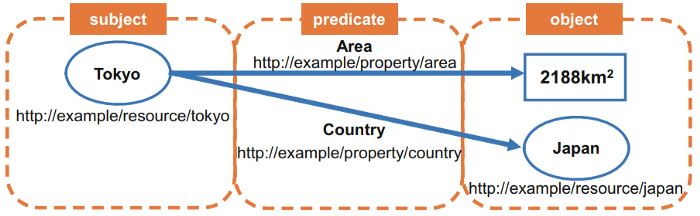
\includegraphics[width = 0.9\textwidth]{images/background/linked-data.png}
    \caption{\gls{RDF} representation of the city Tokyo, with predicates relating it to its area and its country. Source: \citet{generating-pva}}
    \label{fig:linked-data}
\end{figure}

\noindent Subjects, predicates and objects are all identified by a URI, making them universal, and allowing anyone to define new predicates\footnote{Unless they are literals, such as the area in the example}. Like this, webs of information are formed between related objects using definitions that can be found and understood by everyone.

This does not completely solve the problem, however. It is possible that multiple definitions exist for essentially the same object. To resolve this, the Semantic Web introduces a third component: ontologies. Ontologies are documents that formally define the relations among terms \citep{semantic-web}. A widely-used ontology is called \textit{foaf}\footnote{\url{ http://xmlns.com/foaf/spec/}} (friend-of-a-friend): it is used to describe relationships between people.

\gls{RDF}, however, is only something conceptual (a collection of subject, predicate and object). If we want to actually use it, we need to store \gls{RDF} in documents. This is possible in multiple ways, i.e., multiple representation formats exist. The most popular ones are Turtle \citep{turtle} and JSON-LD \citep{jsonld}. Turtle has the advantage that it allows you to define prefixes at the top of the file, which are aliases for the long URIs that you use to relate the subjects/predicates/objects. If you want to talk about the foaf ontology, you can define at the top of your file:

\texttt{@prefix foaf <http://xlmns.com/foaf/0.1/>}

\noindent You can then use \texttt{foaf} in the rest of your turtle file, instead of \texttt{<http://xlmns.com/\\foaf/0.1/>}. This makes it very human-readable compared to other formats. Additional existing formats are \gls{RDF}/XML and N-Triples, but they are less common.

\subsection{The Solid Protocol}
\begin{quote}{\href{https://solidproject.org}{solidproject.org}}
    Solid is a proposed set of conventions and tools for building \textit{decentralized applications} based on Linked Data principles.
\end{quote}
\noindent Solid \citep{solid} is a proposed W3C specification that wishes to decentralize the web by giving people control over their data. Solid aims to realize this by giving people an online datastore called a \textit{pod} (personal online datastore). Users can then login to applications using an authentication mechanism provided by Solid, and the application can in turn access data stored in the user's pod.

By storing all the data inside the user's pod instead of on the application server, the user retains complete control over his data. He can flexibly choose what data to share with what applications. Furthermore, storing the data in a pod reduces vendor lock-in: when the user wishes to switch from one service to another, he can simply give the new application access to the data he already possesses. 
In Solid, there are two types of resources: linked and non-linked data resources. Non-linked data resources are the usual kinds of data that we access on the web right now (binary, text, images, ...), while linked data follows the 
 \gls{RDF} specifications by using a content representation such as Turtle. These linked-data standards follow the principles of the Semantic Web.

\subsection{Authentication}
Authenticating a user is the act of verifying a user's claimed identity. Identities in solid (both for users and other agents) follow the WebID standard \citep{webid}: URIs act as universal identifiers. An example WebID is:

\begin{center}
   \texttt{https://jessegeens.solidcommunity.net/profile/card\#me}\\
\end{center}

\noindent These WebID URIs can identify several things: users, software agents, or other things (even if they do not exist on the web). The WebID URI references a WebID Profile Document. This document contains information about the agent who is the referent of the WebID URI. However, an important distinction must be made. When the \textit{\texttt{\#me}} is included in the URI (or more in general, the hashtag), this URI refers to an agent. When the hashtag is omitted, the URI refers to the document describing this agent.

While the WebID standard provides identities, it does not yet verify them. The actual authentication (or, verifying that the agent actually controls the WebID he claims to control) in Solid uses the WebID-OIDC protocol. This protocol draws inspiration from OAuth2 and from OpenID Connect. The below workflow, drawn from the WebID-OIDC repository, explains the basic mechanism of the protocol:

\todo{Also here, make sure this is not plagiarism, since it is copied from the repo}

\begin{quote}{\href{https://github.com/solid/webid-oidc-spec}{webid-oidc-spec repository}}

    1. \textbf{Initial Request}: Alice (unauthenticated) makes a request to bob.example, receives a \texttt{HTTP 401 Unauthorized} response, and is presented with a 'Sign In With...' screen.\\
    
    2. \textbf{Provider Selection}: She selects her WebID service provider by clicking on a logo, typing in a URI (for example, alice.solidtest.space), or entering her email.\\
    
    3. \textbf{Local Authentication}: Alice gets redirected towards her service provider's own Sign In page, thus requesting https://alice.solidtest.space/signin, and authenticates using her preferred method (password, WebID-TLS certificate, FIDO 2 / WebAuthn device, etc).\\
    
    4. \textbf{User Consent}: (Optional) She's presented with a user consent screen, along the lines of "Do you wish to sign in to bob.example?".\\
    
    5. \textbf{Authentication Response}: She then gets redirected back towards https://bob.example/resource1 (the resource she was originally trying to request). The server, bob.example, also receives a signed ID Token from alice.solidtest.space that was returned with the response in point 3, attesting that she has signed in.\\
    
    6. \textbf{Deriving a WebID URI}: bob.example (the server controlling the resource) validates the ID Token, and extracts Alice's WebID URI from inside it. She is now signed in to bob.example as user https://alice.solidtest.space/\#i.\\
    
    7. \textbf{WebID Provider Confirmation}: bob.example confirms that solidtest.space is indeed Alice's authorized OIDC provider (by matching the provider URI from the iss claim with Alice's WebID).

\end{quote}

\subsection{Authorization}
Authorization within the Solid project builds on the Web Access Control standard \citep{wac}. The WAC standard provides a method to define authorization conditions for resources in a Pod using an \gls{ACL}.\todo{Explain here what an access control list is?} Every resource is coupled with an \gls{ACL} resource - either directly, or by inheriting it from a parent container. These \gls{ACL} resources are using the ACL ontology, usually in a turtle file\footnote{Other \gls{RDF} representations are also allowed, but support for turtle files is mandatory}. Authorization conditions consist of three elements: access objects (the associated resource), access modes (\textit{read}, \textit{write}, \textit{append} or \textit{control}) and access subjects (the agents performing the request).

The access objects in an \gls{ACL} resource are the resources the \gls{ACL} resource refers to. This can be both a normal resource (LDP-RS or LDP-NR, see \ref{subsec:ldp}) as well as a container. It is not mandatory for resources to have an associated ACL resource, as these can be inherited. This mechanism ensures that there is no need to create duplicate ACL resources for similar resources, as well as ensuring proper protection for newly created resources. When a resource is accessed, the server will first look for a directly associated \gls{ACL} resource. When none is found, the server will walk up the container tree (starting from the current container the resource is located in, then the parents, up until the root container). Once an \gls{ACL} resource applying to one of the parent containers is found, this is applied to the requested resource.

Possible access modes, then, are either \textit{read}, \textit{write}, \textit{append} or \textit{control}. Reading and writing are the usual operations. Append is a subset of writing: data can be added to the resource, but not deleted. This is useful for, for example, logging applications, ensuring that logs cannot be removed. Since appending is a subset of writing, the writing authorization implies the appending authorization (no resource can allow writing but disallow appending). Finally, control means being able to modify the ACL of the resource. Being able to control a resource generally implies ownership of the resource.

Lastly, access subjects are those agents who request a certain operation on the resource. Generally, these can be divided into four categories. The first one is \textit{every agent}, i.e., the resource is publicly accessible. A second option is authenticated agents only (with no restrictions on who these agents are), which may be useful for auditing purposes. Thirdly, resource access can be restricted to agents with a specific WebID. Finally, this can also be extended to groups of agents (where the group has a single WebID). An example \gls{ACL} resource, taken from the Solid Community Server\footnote{See \url{https://github.com/solid/community-server}}, is presented below:
\lstinputlisting[style=turtle, title=.acl, caption=Access Control List Resource]{code/acl.ttl}

\subsection{Linked Data Platform and Containers}
\label{subsec:ldp}
Solid mainly relies on the \gls{LDP} protocol \citep{ldp} for resource management. The \gls{LDP} protocol uses HTTP for accessing and modifying resources on a server. LDP Resources, or LDPRs, are HTTP resources that conform to a number of conventions. There are multiple types of resources:
\begin{enumerate}
    \item \gls{RDF} Sources, also called LDP-RSs (LDP \gls{RDF} Source)
    \item Non-\gls{RDF} Sources, such as images or binary data, which are called LDP-NRs
    \item Containers, a concept for bundling related resources together. These are also called LDPCs (LDP Container). 
\end{enumerate}

\noindent To support the access and modification of these resources, \gls{LDP} servers must support a number of HTTP methods on the resources. The \texttt{GET} method is mandatory and returns the request resource, if certain conditions are met (e.g., does the agent have the correct authorizations to access the resource). The \texttt{POST} and \texttt{PUT} methods are optional, and allow agents to create new resources or modify existing ones. Similarly, the \texttt{DELETE} method is optional and allows agents to delete resources. The \texttt{HEAD} and \texttt{OPTIONS} methods are mandatory to be implemented by servers and are similar to the methods defined in the HTTP/1.1 protocol. Below is an example of a request for a basic container and the accompanying reply \citep[from][]{ldp-primer}:

\begin{verbatim}
GET /alice/ HTTP/1.1
Host: example.org
Accept: text/turtle
HTTP/1.1 200 OK 
Content-Type: text/turtle; charset=UTF-8
Link: <http://www.w3.org/ns/ldp#BasicContainer>; rel="type", 
      <http://www.w3.org/ns/ldp#Resource>; rel="type"
Allow: OPTIONS,HEAD,GET,POST,PUT,PATCH
Accept-Post: text/turtle, application/ld+json, image/bmp, image/jpeg
Accept-Patch: text/ldpatch
Content-Length: 250
ETag: W/'123456789'
	
@prefix dcterms: <http://purl.org/dc/terms/>.
@prefix ldp: <http://www.w3.org/ns/ldp#>.
	
<http://example.org/alice/> a ldp:Container, ldp:BasicContainer;
  dcterms:title 'Alice`s data storage on the Web' .	
\end{verbatim}

\newpage
\begin{formal}
\textbf{Optional reading} $ - $
\textit{LDP Containers}\\

\noindent LDP Containers are a specialization of a LDP \gls{RDF} Source, which represent a set of links to other LDPRs that are contained within the container. There are multiple types of LDPCs. The simplest one is the Basic Container or LDP-BC. It defines a basic notion of containment using a generic vocabulary and a \texttt{ldp:contains} relationship. In LDP-BCs, there are no restrictions on LDPRs contained within. The figure below illustrates a LDP Basic Container.\\
\phantom{kkkkkkkkk||||||}{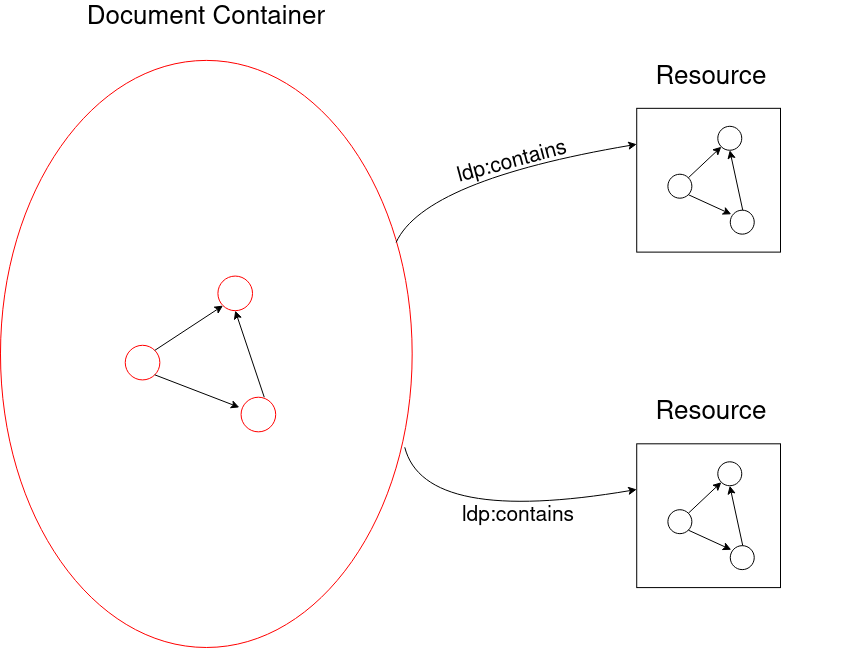
\includegraphics[width=0.60\textwidth]{images/background/ldp-bc.png}}\\
\noindent Direct Containers, or LDP-DCs, are a specialization of a Basic Container. The LDP-DC can make assertions, called membership triples, on resources withing the container. These assertions, which use domain-specific vocabulary, are made as part of the creation process for resources placed in the container. The membership triples do not need to refer to the container resource - these can refer to other resources as well. The figure below illustrates a LDP Basic Container containing movies, and a LDP Direct Container containing documents (images, movies, ..) where the actor is depicted, illustrated through the predicate \texttt{foaf:depicton}. \\
\phantom{kkk|||}{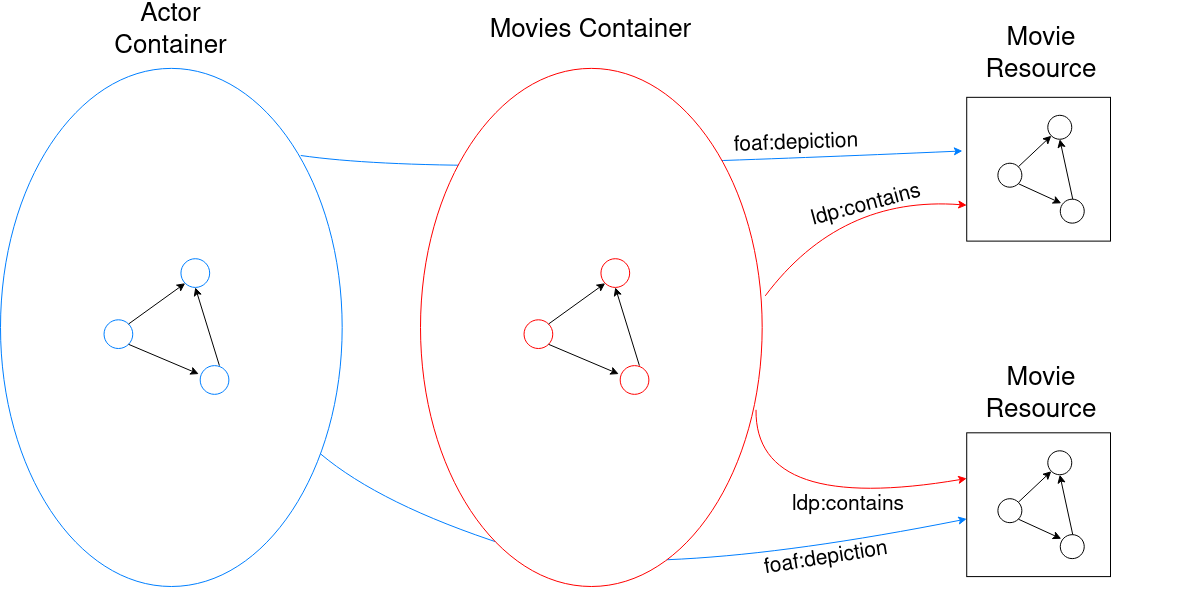
\includegraphics[width=0.9\textwidth]{images/background/ldp-dc.png}}\\

\noindent \textit{Source}: \url{https://www.w3.org/TR/ldp-primer/}
\end{formal}

\newpage
\section{Privacy-Enhancing Technologies}
\label{sec:pets}
\subsection{The need for Privacy-Enhancing Technologies}
The concept of privacy has been around for a long time. Even in the 14th century already, cases were brought before court for eavesdropping and opening letters \citep{privacy-history}. Initially, it was more understood in the context of being let alone, especially in one's house or personal properties. Since the dawn of the information age after the Second World War, the concept started to shift more towards privacy in the context of personal information and publications on the topic started to appear. The definition did not change much however, remaining very similar to the one introduced in 1891 by Warren and Brandeis \citep{privacy-history}:
\begin{quote}{Samuel Warren, Louis Brandeis}
    Privacy is described as a right to be let alone and a right of each individual  to  determine,  under  ordinary  circumstances,  what  his  or  her  thoughts, sentiments, and emotions shall be when in communication with others.
\end{quote}
\todo{Compare with definition of privacy in introduction to PETs, compare inward and outward definition}
\noindent The ubiquity of personal data collection in recent years has strengthened privacy concerns. Especially since the Web has become extremely centralized, with only six companies accounting for 43\% of global internet traffic \citep{internet-report}, there has been a growing demand for technologies that help protect user privacy.

Not only from the data subject's perspective is there a growing concern for data privacy. With the introduction of the \gls{GDPR} in 2018, companies have a legal obligation to take care of user data, especially if it is sensitive. This clashes with the rise of the Saas/PaaS business models, where companies outsource data storage and management. However, this is not always possible and comes with risks. If a Data Processor (a third party that processes data on behalf of a Data Controller) leaks data, the Data Controller risks violating the user's trust (and legal sanctions). \todo{Optional reading or subsection about GDPR to explain basics and terminology?}

In both cases, Privacy-Enhancing Technologies play a big role in reducing the risk of data leaks and preserving user privacy. \citeauthor{pets-handbook} introduced the following definition, which was later adopted by the European Commission\footnote{\url{https://eur-lex.europa.eu/LexUriServ/LexUriServ.do?uri=COM:2007:0228:FIN:EN:PDF}}:
\begin{quote}{\citeauthor{pets-handbook}}
    Privacy-Enhancing Technologies is a system of ICT measures protecting informational privacy by eliminating or minimising personal data thereby preventing unnecessary or unwanted processing of personal data, without the loss of the functionality of the information system.
\end{quote} 
The following sections will introduce a number of widely used \gls{PETs}, some of which will be used in \middleware{}.

\subsection{Data (de-)identification}
\label{sec:data-deid}
The previous section gave an introduction to the concept of privacy. In IT systems, this applies to personal data. But when is data personal? In the context of ePrivacy, the term \textit{\gls{PII}}, is used widely. The term applies to data elements that contain references to attributes that can, either directly or indirectly, disclose someone's identity. A distinction can then be made between three types of data \citep{de-id-taxonomy}:
\begin{itemize}
    \item \textbf{Direct identifiers}: data attributes that directly identify an individual. Examples are national identification numbers, home addresses, e-mail addresses, full names, etc.
    \item \textbf{Indirect identifiers}: data attributes that can be combined with other data attributes to identify an individual, but do not disclose an identity on their own. Examples are birth dates, family names, IP addresses etc.
    \item \textbf{Non-PII elements}: data attributes that contain no reference at all to a person's identity.
\end{itemize}
\noindent \citeauthor{privacy-design-strategies} notes that much like security, privacy is a core property of software systems, and is heavily architecture-dependent. It is therefore of paramount importance that privacy considerations are taken into account from the outset and through the whole development cycle. This design philosophy is named \textit{privacy by design} and it is one of the requirements listed in the GDPR. For regular software design, software developers have used software design patterns to solve common architectural problems. Likewise, \citet{privacy-design-strategies} and \citet{de-id-taxonomy} propose a number of \textit{privacy design strategies}.

\subsection{Transformation-based Approaches}
\label{sec:transformation-approaches}
Transformation-based approaches are approaches that modify datasets in a uniform way, such that the resulting dataset contains less \gls{PII}. Since data transformations \textit{modify} the dataset, it is important to note that this has an impact on the utility of the data. Some transformations may be more powerful at anonymizing the data, but at the same time make the data less valuable or even unusable. A balance must be struck between data privacy and utility, where the choice for a certain data transformation is very context-dependent. This section introduces a number of data transformations.

For an overview of common architectural tactics for data de-identification, we look at the literature study by \citeauthor{de-id-taxonomy}. This study includes 163 investigated articles and builds a taxonomy for data de-identification architectural tactics, mostly consisting of transformation-based approaches. Table \ref{table:de-id-taxonomy} presents their proposed data transformation tactics.
\newpage
\begin{table}[H]
\begin{center}
\begin{tabulary}{\textwidth}{p{0.17\textwidth}p{0.83\textwidth}}
\textbf{Tactic name} & \textbf{Description}                                                                                                                                                          \\ \hline
Remove               & The targeted and deliberate omission of PII from the data record or data set.                                                                                                 \\
Select / Filter      & Same as Remove applied to a copy of the data while keeping the original data.                                                                                                 \\
Transform            & The application of a holistic transformation (not targeted on PII elements only) on data elements that is destructive in terms of ability to distinguish these data elements. \\
Mask                 & Overwriting data elements with other values for the purpose of obfuscating the content.                                                                                       \\
Encrypt              & Using cryptographic means to encode the PII attribute values / records / datasets.                                                                                            \\
Randomize            & Tactics that involve the modification of PII attribute values/records by injecting artificial random elements.                                                                \\
Aggregate            & Generalize, combine and group data elements.                                                                                                                                  \\
Blur                 & Reduce the accuracy of the data so that distinguishing characteristics become indiscernible.                                                                                  \\
Pseudonym            & The systematic replacement of direct identifiers with surrogates, whereby the mapping between surrogate and identity is kept separately.                                      \\
Placeholder          & The systematic replacement of direct identifiers with a surrogate that is the same for all members of the population.                                                         \\
Interchange          & The targeted mingling of data elements across members of the population.                                                                                                      \\
Synthetic            & The replacement of data elements with a synthetic placeholder which is a constructed representation specifically aimed at conveying discriminatory features.                 
\end{tabulary}
\caption{Overview of architectural tactics involving data transformations, by \citet{de-id-taxonomy}}
\label{table:de-id-taxonomy}
\end{center}
\end{table}

\subsection{Encrypted Database Systems}\todo{Can I just import table like this (plagiarism/copyright)?}\todo{Do generalisations, such as going from city to province, fall under aggregate?}
Encrypted Database Systems are database systems that store encrypted data, while maintaining some functionality. It is a vast research field, with \citet{sok-cryptdb} being a formative work. The need for encrypted database systems arises from the rise of the PaaS\footnote{Platform-as-a-Service} model, whereby software and database deployment is outsourced to third parties such as Amazon Web Services and others. \todo{Finish paragraph, explain things like leakage}

Many types of encryption exist for these database systems, ranging from very secure to less secure, but in turn providing more functionality. Popular encryption schemes, sorted from least to most leakage, are \citep{cryptdice}:
\begin{itemize}
    \item \textbf{Random/probabilistic encryption}: Random encryption is an encryption scheme in which encrypting the same plaintext results in a different ciphertext. This is usually achieved by making use of the AES encryption scheme, and using a randomly generated Initialization Vector (IV). This scheme provides the strongest data protection, but it offers no useful operations on the data.
    \item \textbf{Deterministic encryption}: Deterministic encryption works similar to random encryption, but now the IV is kept constant. This results in a scheme which gives the same ciphertext for the same plaintext input. This is less secure, but allows for equality comparisons.
    \item \textbf{Order-preserving encryption}: In the order-preserving encryption scheme, the order relationship between plaintext is preserved in the ciphertext. Therefore, it is possible to do order-comparisons between encrypted data elements, allowing functionality such as range queries.
    \item \textbf{Order-revealing encryption}: Order-revealing encryption is an outdated form of order-preserving encryption. Its usage is discouraged, since it has a larger leakage then order-revealing encryption while providing the same level of functionality. \todo{Add citation here}
\end{itemize}
A new type of encryption scheme that has recently started to become popular is \textit{homomorphic encryption}: it allows processing on encrypted data by supporting mathematical operations on the encrypted data, such as multiplication and addition. It has become popular over the last decade, with \citet{fhe} being a breakthrough work and Google recently releasing a open-source library\footnote{\url{https://github.com/google/fully-homomorphic-encryption}} supporting fully homomorphic encryption. While Somewhat Homomorphic Encryption already has practical applications, this is less the case for Fully Homomorphic Encryption, with the main hurdle being that it is very computationally intensive.
\begin{itemize}
    \item \textbf{Somewhat Homomorphic Encryption}: Somewhat homomorphic encryption schemes, also called partially homomorphic encryption schemes, are homomorphic encryption schemes that support either addition or multiplication, but not both \citep{she}. An example of a additive homomorphic encryption scheme is the Paillier Cryptosystem \citep{paillier}. A widely used multiplicative homomorphic encryption scheme is the ElGamal CryptoSystem \citep{elgamal}.
    \item \textbf{Fully Homomorphic Encryption}: Fully homomorphic encryption schemes are homomorphic encryption schemes that support both addition and multiplication on encrypted data. This is incredibly powerful, since any function can be represented as a circuit consisting of multiplication and addition gates. It can, theoretically, thus compute any function over encrypted data. However, it is still too computationally intensive for a number of practical applications \citep{he-practical, pragmatic-mpc}. Despite that hurdle it remains a promising technology, allowing applications such as encrypted search queries \citep{fhe}, and every year more efficient implementations are proposed.
\end{itemize}
\subsection{Other Approaches}
\subsubsection{Secure Multi-Party Computation}
\label{sec:mpc}
\gls{MPC} is an exciting research field that has seen a large amount of research over the last few decades, while the techniques and modern computers have only recently evolved enough to allow practical applications. It is a technique that allows any number of parties to secretly compute any function over some encrypted input data, while only revealing the requested output to the parties. The basic techniques for Multi-Party Computation stem from a groundbreaking paper by \citet{yao} (for two-party computation), which was later extended to the multi-party case by \citet{mpc}.

\gls{MPC} has a somewhat unusual security model, since the adversary can be a party to the computation instead of being an outsider. The adversary model thus considers some adversarial entity, which manages to exert control over a subset of the parties partaking in the computation. Such a controlled party is called \textit{corrupted}. Often, a \textit{monolithic adversary} is considered: if there are multiple corrupted parties, it is assumed they work together \citep{mpc-good-practice}. When an adversary controls multiple corrupted parties, several \textit{corruptions strategies} are possible \citep{secure-mpc}. In the \textit{static corruption model}, the set of corrupted parties is fixed from the onset and does not change during execution of the protocol. In the \textit{adaptive corruption model}, the adversary can corrupt parties during the execution, but once a party has been corrupted it remains corrupted until the end of the protocol. Finally, there is the \textit{proactive security model} \citep{sec-transient-failures}, where corrupted parties can become honest again (for example, because a breach has been detected and the systems are recovered).\todo{Too detailed?}

Of course, many protocols exist for facilitating computation between multiple parties, even HTTP would support that. The goal of \gls{MPC} is to provide a \textit{secure} protocol. Often, the \textit{real-ideal}\footnote{In the real-ideal security definition, an adversary can not harm the real protocol more than what would be possible in an ideal protocol \citep{mpc}} definition of security is taken to define when such a system is secure. However, this does not provide many practical guidelines. \citet{secure-mpc} lists a number of minimal (but not exhaustive) requirements, which every secure protocol should fulfill:

\begin{quote}{\citet[p.2]{secure-mpc}}
\begin{enumerate}
    \item \textbf{Privacy}: No party should learn anything more than its prescribed output.
    \item \textbf{Correctness}: Each party is guaranteed that the output it receives is correct.
    \item \textbf{Independence of Inputs}: Corrupted parties must choose their inputs independently of the honest parties' inputs.
    \item \textbf{Guaranteed Output Delivery}: Corrupted parties should not be able to prevent honest parties from receiving their output.
    \item \textbf{Fairness}: Corrupted parties should receive their outputs if and only if the honest parties also receive their outputs.
\end{enumerate}
\end{quote}
The actual computation, then, is usually based on something called a \textit{garbled circuit}, introduced by \citeauthor{yao}\todo{add citation for garbled circuits}. The function to be computed is represented as a boolean circuit where the gates are encrypted. \todo{source}The explanation of the complete protocol is out of the scope for this thesis, but it is described in \citet{secure-mpc, pragmatic-mpc} and uses techniques such as Oblivious Transfer\todo{cite}. For some use-cases, generic \gls{MPC} protocols may not be the most efficient and specific protocols that are much faster may exist. A very common example is Private Set Intersection\todo{cite, add acronym}.

\subsubsection{Differential Privacy \& \textit{k}-Anonymity}
Differential privacy and \textit{k}-Anonymity are both types of \textit{statistical} privacy. 

In differential privacy, participating in a database does not substantially increase the risk to the user's privacy \citep{diff-privacy}. \todo{Look later at this paper, it provides some references to proofs that non-interactive (ie data transformations) work less well than interactive approaches, because at the time of the sanitization the future utility is not always known yet. Then discuss that statistical methods cannot be used since we only have data from one user.} This definition follows from \citeauthor{diff-privacy}'s impossibility proof of absolute disclosure prevention. She proved that even if a database has very little information (such as the average height of a person for every country), even that information can lead to a privacy breach in the presence of side information. Imagine that a person's height is sensitive information, and that it is known that Alice's height is 2cm less than the average height. Then the database containing average heights discloses Alice's height, leading to a privacy breach. Because this is impossible to circumvent, \citeauthor{Dwork} introduces the relative notion: a disclosure is just as likely whether the individual takes part in the database or not. In short, the technique works by adding specifically chosen random noise to the answer of a query, to statistically provide the \textit{$\epsilon$}-differential privacy guarantees. A more rigorous explanation can be found in \citet[p9-11]{diff-privacy}.

\textit{k}-Anonymity was introduced by \citet{k-anonymity}, who defined it in terms of de-identifying persons from so-called \textit{quasi-identifiers} (i.e. indirect identifiers) in released data sets. \citet{demographics-identify-unique} notes that 53\% of the U.S. population can be uniquely identified with only the following attributes: place, gender and date of birth. In this context, it is very difficult to correctly identify indirect identifiers, since it is not known beforehand with which data this can be combined to determine unique identities. If a dataset is \textit{k}-anonymous, however, it is impossible (even when combining with another dataset), to uniquely identify individuals. A data release is \textit{k}-anonymous if "the information for each person contained in the release cannot be distinguished from at least \textit{k}-1 individuals whose information also appears in the release" \citep{k-anonymity}. Thus, every unique combination of identifiers maps to at least \textit{k} individuals, making individual identification unlikely\footnote{There exist attacks on \textit{k}-anonymity, but most can be resisted by following the accompanying policies stipulated in \citet{k-anonymity}.}.

\subsection{Related works}\todo{Is this section useful? Or does the general text already give enough references to related works?}
\noindent \textbf{CryptDB} \citep{cryptdb} is a seminal work in the research field of encrypted database systems. It is a SQL database that allows queries over encrypted data. Its main contributions are the demonstration of two new techniques, \textit{adjustable query-based encryption} and \textit{encryption key chaining}. 

Adjustable query-based encryption is a technique that dynamically adapts the the encryption scheme of columns based on queries: it automatically selects the highest possible security given the queries that need to be executed on that column. It does this in a two-fold manner. Firstly, different columns (and tables) have different encryption keys, so that the encryption level can be varied on data fields (some columns might be more sensitive and thus require stronger encryption). Secondly, CryptDB encrypts columns in an \textit{onion}: when the database is initialized, every column is encrypted several times, each time with a stronger encryption mechanism. When a query is then executed against a column whose strong encryption scheme is not compatible with the query, layers are removed until a compatible encryption scheme is reached. 

Encryption key chaining then, is a method to cryptographically enforce access control policies. In CryptDB, principals (either users or groups of users) all have their own key. \citeauthor{cryptdb} developed a novel way to encrypt data such that only the correct principals have access to the data, by making use of both symmetric and asymmetric keys: they use symmetric keys when both users are online, so an interim key can be stored in memory, or asymmetric encryption when one of the users is not online. This strikes a balance between security (only current keys of online users can be leaked in case of an attack) and performance (as symmetric encryption is much more performant). The technique itself requires some background information and can thus be found in the paper itself.\todo{This paragraph does not bring over the idea well, so should be rewritten later}\\

\noindent \textbf{DataBlinder}, by \citet{datablinder}, presents ... \todo{Write more about related works}\\

\noindent \textbf{Cryptdice} \citep{cryptdice} illustrate ...\\

\noindent \textbf{Secure Multi-Party Computation} \citep{secure-mpc} gives a good overview of\\


\chapter{Analysis}
\label{chap:analysis}
This chapter studies a wide range of \gls{PETs}, discussing how they work and analyzing whether they are applicable in the context of a decentralized middleware for enhancing data privacy in Solid. Based on this analysis, a number of \gls{PETs} will be chosen to be supported in \middleware{}. 

\section{Transformation-based approaches}
\label{sec:transformation-approaches}
Transformation-based approaches are approaches that modify datasets in a uniform way (on a by-row basis), such that the resulting dataset contains less \gls{PII}. Since data transformations \textit{modify} the dataset, it is important to note that this has an impact on the utility of the data. Some transformations may be more powerful at anonymizing the data, but at the same time make the data less valuable or even unusable. A balance must be struck between data privacy and utility, where the choice for a certain data transformation is very context-dependent. This section introduces a number of data transformations.

For an overview of common architectural tactics for data de-identification, we look at the literature study by \citeauthor{de-id-taxonomy}. This study includes 163 investigated articles and builds a taxonomy for data de-identification architectural tactics, mostly consisting of transformation-based approaches. Table \ref{table:de-id-taxonomy} presents their proposed data transformation tactics.

Such transformations seem very usable in the context of a middleware that anonymizes data. They are often fairly simple transformations, that can range in privacy strength and resulting utility. Because these transformations are so dynamic, they are perfect to adapt to different trust levels of applications, allowing more impactful transformations on data sent to applications that are less trusted. Another big advantage of an approach taking advantage of data transformations is that this can be realised statelessly. As the data is sanitized on a record-by-record basis, independently of the other records, there is no need to keep track of state. This heavily simplifies possible architectural designs.
\newpage
\begin{table}[H]
\begin{center}
\begin{tabulary}{\textwidth}{p{0.17\textwidth}p{0.83\textwidth}}
\textbf{Tactic name} & \textbf{Description}                                                                                                                                                          \\ \hline
Remove               & The targeted and deliberate omission of PII from the data record or data set.                                                                                                 \\
Select / Filter      & Same as Remove applied to a copy of the data while keeping the original data.                                                                                                 \\
Transform            & The application of a holistic transformation (not targeted on PII elements only) on data elements that is destructive in terms of ability to distinguish these data elements. \\
Mask                 & Overwriting data elements with other values for the purpose of obfuscating the content.                                                                                       \\
Encrypt              & Using cryptographic means to encode the PII attribute values / records / datasets.                                                                                            \\
Randomize            & Tactics that involve the modification of PII attribute values/records by injecting artificial random elements.                                                                \\
Aggregate            & Generalize, combine and group data elements.                                                                                                                                  \\
Blur                 & Reduce the accuracy of the data so that distinguishing characteristics become indiscernible.                                                                                  \\
Pseudonym            & The systematic replacement of direct identifiers with surrogates, whereby the mapping between surrogate and identity is kept separately.                                      \\
Placeholder          & The systematic replacement of direct identifiers with a surrogate that is the same for all members of the population.                                                         \\
Interchange          & The targeted mingling of data elements across members of the population.                                                                                                      \\
Synthetic            & The replacement of data elements with a synthetic placeholder which is a constructed representation specifically aimed at conveying discriminatory features.                 
\end{tabulary}
\caption{Overview of architectural tactics involving data transformations, by \citet{de-id-taxonomy}}
\label{table:de-id-taxonomy}
\end{center}
\end{table}

\section{Encrypted Database Systems}\todo{Can I just import table like this (plagiarism/copyright)?}\todo{Do generalisations, such as going from city to province, fall under aggregate?}
Encrypted Database Systems are database systems that store encrypted data, while maintaining some functionality over this data. It is a vast research field, with \citet{sok-cryptdb} being a formative work. The need for encrypted database systems arises from the rise of the PaaS\footnote{Platform-as-a-Service} model, whereby software and database deployment is outsourced to third parties such as Amazon Web Services and others. Since these "cloud platforms" store sensitive data (customer data, economically valuable information, ...), it is important for certain users to guarantee that these providers are unable to access their stored data. This is realised by encrypting the data, but this brings along problems. Since these databases are often very large, information is retrieved through complex queries. These queries may not support operating on encrypted data by default, so some new techniques are necessary.

Many types of encryption exist for these database systems, ranging from very secure to less secure, but in turn providing more functionality. Popular encryption schemes, sorted from least to most leakage, are \citep{cryptdice}:
\begin{itemize}
    \item \textbf{Random/probabilistic encryption}: Random encryption is an encryption scheme in which encrypting the same plaintext results in a different ciphertext. This is usually achieved by making use of the AES encryption scheme, and using a randomly generated Initialization Vector (IV). This scheme provides the strongest data protection, but it offers no useful operations on the data.
    \item \textbf{Deterministic encryption}: Deterministic encryption works similar to random encryption, but now the IV is kept constant. This results in a scheme which gives the same ciphertext for the same plaintext input. This is less secure, but allows for equality comparisons.
    \item \textbf{Order-preserving encryption}: In the order-preserving encryption scheme, the order relationship between plaintext is preserved in the ciphertext. Therefore, it is possible to do order-comparisons between encrypted data elements, allowing functionality such as range queries.
    \item \textbf{Order-revealing encryption}: Order-revealing encryption is an outdated form of order-preserving encryption. Its usage is discouraged, since it has a larger leakage then order-revealing encryption while providing the same level of functionality. \todo{Add citation here}
\end{itemize}
A new type of encryption scheme that has recently started to become popular is \textit{homomorphic encryption}: it allows processing on encrypted data by supporting mathematical operations on the encrypted data, such as multiplication and addition. It has become popular over the last decade, with \citet{fhe} being a breakthrough work and Google recently releasing an open-source library\footnote{\url{https://github.com/google/fully-homomorphic-encryption}} supporting fully homomorphic encryption. While Somewhat Homomorphic Encryption already has practical applications, this is less the case for Fully Homomorphic Encryption, with the main hurdle being that it is very computationally intensive.
\begin{itemize}
    \item \textbf{Somewhat Homomorphic Encryption}: Somewhat homomorphic encryption schemes, also called partially homomorphic encryption schemes, are homomorphic encryption schemes that support either addition or multiplication, but not both \citep{she}. An example of a additive homomorphic encryption scheme is the Paillier Cryptosystem \citep{paillier}. A widely used multiplicative homomorphic encryption scheme is the ElGamal CryptoSystem \citep{elgamal}.
    \item \textbf{Fully Homomorphic Encryption}: Fully homomorphic encryption schemes are homomorphic encryption schemes that support both addition and multiplication on encrypted data. This is incredibly powerful, since any function can be represented as a circuit consisting of multiplication and addition gates. It can, theoretically, thus compute any function over encrypted data. However, it is still too computationally intensive for a number of practical applications \citep{he-practical, pragmatic-mpc}. Despite that hurdle it remains a promising technology, allowing applications such as encrypted search queries \citep{fhe}, and every year more efficient implementations are proposed.
\end{itemize}

\noindent While Encrypted Database Systems form a very active research domain, it is less applicable when the focus is on giving data to untrusted applications. These applications need the data by definition, and the goal is to give them modified datasets resulting in less leakage. In contrast, Encrypted Databases are applicable when the \textit{storage provider} is untrusted, instead of the application. This is especially the case for non-homomorphic encryption. 

Homomorphic encryption is also not applicable in the scope of what this thesis researches, however, it may be interesting future work. Homomorphic encryption could be used to give some encrypted data to an application that then performs computations on it. These computations could then be returned to the component that encrypted them, decrypting the results before storing them in the Solid server again. This way, secure computations on data could be supported in the Solid ecosystem.\todo{Reference as future work!}

\section{Secure Multi-Party Computation}
\label{sec:mpc}
\gls{MPC} is an exciting research field that has seen a large amount of research over the last few decades, while the techniques and modern computers have only recently evolved enough to allow practical applications. It is a technique that allows any number of parties to secretly compute any function over some encrypted input data, while only revealing the requested output to the parties. The basic techniques for Multi-Party Computation stem from a groundbreaking paper by \citet{yao} (for two-party computation), which was later extended to the multi-party case by \citet{mpc}.

\gls{MPC} has a somewhat unusual security model, since the adversary can be a party to the computation instead of being an outsider. The adversary model thus considers some adversarial entity, which manages to exert control over a subset of the parties partaking in the computation. Such a controlled party is called \textit{corrupted}. Often, a \textit{monolithic adversary} is considered: if there are multiple corrupted parties, it is assumed they work together \citep{mpc-good-practice}. When an adversary controls multiple corrupted parties, several \textit{corruptions strategies} are possible \citep{secure-mpc}. In the \textit{static corruption model}, the set of corrupted parties is fixed from the onset and does not change during execution of the protocol. In the \textit{adaptive corruption model}, the adversary can corrupt parties during the execution, but once a party has been corrupted it remains corrupted until the end of the protocol. Finally, there is the \textit{proactive security model} \citep{sec-transient-failures}, where corrupted parties can become honest again (for example, because a breach has been detected and the systems are recovered).\todo{Too detailed?}

Of course, many protocols exist for facilitating computation between multiple parties, even HTTP would support that. The goal of \gls{MPC} is to provide a \textit{secure} protocol. Often, the \textit{real-ideal}\footnote{In the real-ideal security definition, an adversary can not harm the real protocol more than what would be possible in an ideal protocol \citep{mpc}} definition of security is taken to define when such a system is secure. However, this does not provide many practical guidelines. \citet{secure-mpc} lists a number of minimal (but not exhaustive) requirements, which every secure protocol should fulfill:

\begin{quote}{\citet[p.2]{secure-mpc}}
\begin{enumerate}
    \item \textbf{Privacy}: No party should learn anything more than its prescribed output.
    \item \textbf{Correctness}: Each party is guaranteed that the output it receives is correct.
    \item \textbf{Independence of Inputs}: Corrupted parties must choose their inputs independently of the honest parties' inputs.
    \item \textbf{Guaranteed Output Delivery}: Corrupted parties should not be able to prevent honest parties from receiving their output.
    \item \textbf{Fairness}: Corrupted parties should receive their outputs if and only if the honest parties also receive their outputs.
\end{enumerate}
\end{quote}
The actual computation, then, is usually based on something called a \textit{garbled circuit}, introduced by \citeauthor{yao}\todo{add citation for garbled circuits}. The function to be computed is represented as a boolean circuit where the gates are encrypted. \todo{source}The explanation of the complete protocol is out of the scope for this thesis, but it is described in \citet{secure-mpc, pragmatic-mpc} and uses techniques such as Oblivious Transfer\todo{cite}. For some use-cases, generic \gls{MPC} protocols may not be the most efficient and specific protocols that are much faster may exist. A very common example is Private Set Intersection\todo{cite, add acronym}.

\todo[inline]{Add explanation why MPC is not suitable for our middleware}

\section{Differential Privacy \& \textit{k}-Anonymity}
Differential privacy and \textit{k}-Anonymity are both types of \textit{statistical} privacy. 

In differential privacy, \textit{"participating in a database does not substantially increase the risk to the user's privacy"} \citep{diff-privacy}. \todo{Look later at this paper, it provides some references to proofs that non-interactive (ie data transformations) work less well than interactive approaches, because at the time of the sanitization the future utility is not always known yet. Then discuss that statistical methods cannot be used since we only have data from one user.} This definition follows from \citeauthor{diff-privacy}'s impossibility proof of absolute disclosure prevention. She proved that even if a database has very little information (such as the average height of a person for every country), even that information can lead to a privacy breach in the presence of side information. Imagine that a person's height is sensitive information, and that it is known that Alice's height is 2cm less than the average height. Then the database containing average heights discloses Alice's height, leading to a privacy breach. Because this is impossible to circumvent, \citeauthor{diff-privacy} introduces the relative notion: a disclosure is just as likely whether the individual takes part in the database or not. In short, the technique works by adding specifically chosen random noise to the answer of a query, to statistically provide the \textit{$\epsilon$}-differential privacy guarantees. A more rigorous explanation can be found in \citet[p9-11]{diff-privacy}.

\textit{k}-Anonymity was introduced by \citet{k-anonymity}, who defined it in terms of de-identifying persons from so-called \textit{quasi-identifiers} (i.e. indirect identifiers) in released data sets. \citet{demographics-identify-unique} notes that 53\% of the U.S. population can be uniquely identified with only the following attributes: place, gender and date of birth. In this context, it is very difficult to correctly identify indirect identifiers, since it is not known beforehand with which data this can be combined to determine unique identities. If a dataset is \textit{k}-anonymous, however, it is impossible (even when combining with another dataset), to uniquely identify individuals. A data release is \textit{k}-anonymous if "the information for each person contained in the release cannot be distinguished from at least \textit{k}-1 individuals whose information also appears in the release" \citep{k-anonymity}. Thus, every unique combination of identifiers maps to at least \textit{k} individuals, making individual identification unlikely\footnote{There exist attacks on \textit{k}-anonymity, but most can be resisted by following the accompanying policies stipulated in \citet{k-anonymity}.}.

\todo[inline]{Add better explanation using the class from Privacy-Preserving Technologies}

While both technologies are very interesting, there are a number of crucial aspects that stop them from being usable in \middleware{}. First of all, both methods are applicable in datasets with \textit{multiple} users. There is no point in using these methods on data originating from a single user. For differential privacy, this is because it is defined as your participation in the database having a negligible impact (defined by $\epsilon$). However, when the database only consists of records belonging to a single user, this is impossible. On the other hand, \textit{k}-Anonymity lacks that it focuses on a different aspect than what \middleware{} tries to achieve. This is because \textit{k}-Anonymity focuses on preventing \textit{identity disclosure}, while \middleware{} aims to lower the risks of \textit{attribute disclosure}. 

\section{Related works}\todo{Is this section useful? Or does the general text already give enough references to related works? And where does it belong, in the beginning or at the end?}
\noindent \textbf{CryptDB} \citep{cryptdb} is a seminal work in the research field of encrypted database systems. It is a SQL database that allows queries over encrypted data. Its main contributions are the demonstration of two new techniques, \textit{adjustable query-based encryption} and \textit{encryption key chaining}. 

Adjustable query-based encryption is a technique that dynamically adapts the the encryption scheme of columns based on queries: it automatically selects the highest possible security given the queries that need to be executed on that column. It does this in a two-fold manner. Firstly, different columns (and tables) have different encryption keys, so that the encryption level can be varied on data fields (some columns might be more sensitive and thus require stronger encryption). Secondly, CryptDB encrypts columns in an \textit{onion}: when the database is initialized, every column is encrypted several times, each time with a stronger encryption mechanism. When a query is then executed against a column whose strong encryption scheme is not compatible with the query, layers are removed until a compatible encryption scheme is reached. 

Encryption key chaining then, is a method to cryptographically enforce access control policies. In CryptDB, principals (either users or groups of users) all have their own key. \citeauthor{cryptdb} developed a novel way to encrypt data such that only the correct principals have access to the data, by making use of both symmetric and asymmetric keys: they use symmetric keys when both users are online, so an interim key can be stored in memory, or asymmetric encryption when one of the users is not online. This strikes a balance between security (only current keys of online users can be leaked in case of an attack) and performance (as symmetric encryption is much more performant). The technique itself requires some background information and can thus be found in the paper itself.\todo{This paragraph does not bring over the idea well, so should be rewritten later}\\

\noindent \textbf{DataBlinder}, by \citet{datablinder}, presents ... \todo{Write more about related works}\\

\noindent \textbf{Cryptdice} \citep{cryptdice} illustrate ...\\

\noindent \textbf{Secure Multi-Party Computation} \citep{secure-mpc} gives a good overview of\\


\chapter{Requirements}
\label{cha:middleware}
The Solid project aims to solve the problem of decentralizing the web by giving data back to the user. However, no distinction is made between the trust level given to client applications. \middleware{} tries to mitigate this by providing an additional software layer in between the client and Solid server, which provides more fine-grained privacy control options. This problem statement determines the general goals of \middleware{}, but in order to guide the design effectively, some concrete requirements are needed, both non-functional, functional, and from a privacy-perspective. To adequately come up with requirements, we guide the process by making use of two concrete example use-cases, listed in \ref{sec:usecases}.   \todo{Needs more detailed description}

\section{Use cases}
\label{sec:usecases}
\subsection{Exercise}
The anonymization of data including health-related attributes makes a very good use-case to guide the design and development of \middleware{}, since those attributes are sensitive personal information. In this use-case, exercise data from an application such as Strava is stored on the user's Solid pod. He wishes to export this data to a ranking board application to see who of his friends runs the fastest. However, he does not wish to share his exact heart rate since this is sensitive data. Since no suitable linked-data format for running exercises was found (i.e., one that supports all the necessary fields such as heart rate), the \gls{TCX} file format\footnote{Schema: \url{https://www8.garmin.com/xmlschemas/TrainingCenterDatabasev2.xsd}} is used instead. An additional advantage of this format is that it is supported by popular tools such as Strava and can be imported/exported by exercise trackers such as Garmin devices. Unfortunately, this is not a linked-data format, which is a bit contrary to the Solid philosophy. However, it is perfectly supported by solid, and it is a well-known and open format, so it is a .. \todo{Juist verwoorden, het is een "sacrifice" die moet gemaakt worden, die de use-case veel praktischer maakt met de kost dat het geen LD format is}.

\subsection{Personal finance}
In this use-case, the user has stored all his transactions on his Solid pod, and he wishes to see some trends and statistics about his spendings. An example of such a statistic is "how much do I spend on groceries every week?".  However, expenses are very sensitive data, especially when these are exact numbers and store locations. Therefore, the user opts to use \middleware{} to filter out the most sensitive information yet still receive relevant statistics. This is done by removing direct identifiers, and aggregating indirect identifiers, such as store locations and exact spendings at individual transactions.  For example, for entries of the type "Alice spent \texteuro 5,82 at Colruyt Leuven on 8/11/2021 16:53", the user wishes to modify this into "User87532 spent \texteuro 5 at Supermarket on 8/11/2021". This way, trends in the spending are kept (by rounding exact amounts to nearby integers, and replacing exact stores with store types). Information such as "you spent \texteuro 400 in supermarkets this month" will still be available (and relatively accurate), without giving away exact details. An example personal finance app, running on Solid, is \href{https://github.com/solid/money-pane}{money-pane}. Like in the last use-case, unfortunately no suitable linked-data format was found, and a proprietary data format must be used. 
However, the usage of linked-data formats does not have any influences on the developed architecture, and have no influence of the developed proof-of-concept, since the developed architecture is independent of the chosen content-representation.


\section{Non-functional Requirements}
\todo[inline]{Right now, only non-functional requirements and none of them are SMART (specific, measurable, ...). Is this enough?}

As a first step in the development process of the proposed solution, a number of requirements are brought forth to ensure that \middleware{} follows the philosophy of Solid, and to guarantee that solves the problem statement.\todo{Rewrite this sentence}

Since \middleware{} builds forth upon the Solid project, it is crucial that it follows the same philosophy. A core property of Solid is its \textbf{decentralization}, meaning that anyone can run a Solid server and host their pod themselves. Since other users may prefer to use a pod from a provider such as Inrupt\footnote{\url{https://inrupt.com}}, \middleware{} must be able to be run stand-alone. This ensures that 
everyone can run \middleware{} and users are not stuck using the same provider for both their pod and \middleware{}. This comes at a certain performance cost (twice the number of HTTP requests instead of treating the data locally at the Solid server, among a number of other performance inhibitors). However, since decentralization is such a core concept of Solid, .. \todo{juist verwoorden dat ik geloof dat het een sacrifice is die het waard is om te maken, maar dat ander onderzoek mogelijk is om een gelijkaardig concept binnen de bestaande community server te bouwen}.

Solid builds further upon the principles of Linked Data, and Solid servers can store any type of data. As \middleware{} aims to be a general solution, it should work in every case where a Solid server following the specification works, it must provide a way to anonymize \textit{any} type of data. Thus, \textbf{flexibility for the supported data scheme} is an essential part of \middleware{}. Concretely, \middleware{}'s core should not hard-code any supported data schemes and which PET should be applied to them: these should be able to be plugged in flexibly and selected automatically, to ensure that any data scheme can be supported. This provides a technical challenge, as a sufficient level of abstraction must be developed to be able to support any data scheme, while ensuring that the leakage requirements are not violated.

Different client applications may be trusted differently, just as that different data schemes may contain more or less sensitive data elements. An important aspect to solve is thus being able to distinguish different \textit{privacy levels}: required levels of anonymization. \middleware{} must therefore not only be able to adapt to different data schemes, but must also support different privacy levels for every data scheme. The selected PET is highly dependent on the data scheme\todo{explain why, ie sometimes better to delete data, other times pseudonym, or generalise} and required level of privacy, therefore \middleware{} must \textbf{automatically select \gls{PETs}} based on the input data scheme and requested privacy level.

Finally, Solid aims to become the de facto standard for web applications in the future. Consequently, it must be intuitive for non-technical users. There can be no technical jargon, and it must be incredibly easy to set-up. Since \middleware{} aims to follow this philosophy, the proposed solution must be \textbf{intuitive to use} for non-technical users. Concretely, this means that it should be opaque to the users which concrete PET is applied for which use case. On that account, a number of \textit{privacy levels} will be created and presented to the user in a simple manner: a higher privacy level means more data protection but less utility. The user will then be able to select between a number of privacy levels, without needing to understand the technical details behind the scenes. Section \ref{sec:privacylevels} introduces four privacy levels that are used in the developed proof-of-concept, but these serve only as a concrete example. Different users may want different levels of granularity and experts in the field may be able to more rigorously define such levels. Therefore, the supported number of levels must be dynamic as well.

\section{Adversary model}
\todo[inline]{Write here a paragraph about the considered adversary model, decide what leakage is allowed, maybe introduce concept of privacy levels here, ...}

\section{Privacy levels}
\label{sec:privacylevels}
\todo[inline]{see feedback Dimitri, better to define these in terms of maximum allowed leakage}
In order to provide an intuitive mechanism for selecting which data is transformed, different privacy levels are introduced. These privacy levels form an abstraction above the concrete data transformations and \gls{PETs} that are applied to the data before it is passed on to the application. This ensures that non-technical users can use \middleware{}, without needing to know the technical details of the technologies and tactics that are employed. Four levels of increasing privacy are proposed, based partially on the \gls{GDPR} definition of sensitive personal data and on the types of identifiers defined in section \ref{sec:data-deid}.\\

\noindent \textbf{Level 1: all data} No data transformations are applied, all data is passed to the requesting application.\\

\noindent \textbf{Level 2: Removal of sensitive personal data} Sensitive personal data, as defined by the GDPR \citep{gdpr}, is removed from the dataset. This includes data consisting of racial or ethnic origin, political opinions, religious or philosophical beliefs, or trade union membership, genetic data, biometric data, data concerning health, data concerning criminal convictions or data concerning a natural person's sex life or sexual orientation. Thus, the tactic \textit{Remove} is applied to all data elements matching this definition.\todo{Explain why remove is the best tactic here}\\

\noindent \textbf{Level 3: Pseudonymization/generalisation of direct identifiers} Since level 3 is a stronger version of level 2, sensitive personal data is removed first. Additionally, direct personal identifiers are pseudonymized or generalized. Concretely, the tactics \textit{Pseudonym}, \textit{Placeholder}, \textit{Aggregate} and \textit{Blur} may be applied here, depending on the specific data attribute. In addition, data elements may also be \textit{perturbed}. Examples are the replacement of names by placeholders, the perturbation or adding a placeholder for birth dates (such that the exact date is obscured, but the age is still correct), the removal of street names and numbers while keeping larger geographic areas such as cities, etc. This makes the data still relatively accurate, while direct identification of the user is made impossible.\\

\noindent \textbf{Level 4: Pseudonymization/generalisation of (in)direct identifiers} In addition to direct identifiers, also indirect identifiers are now modified or removed. The same \gls{PETs} and tactics are used, but are now applied more strictly and to more data attributes. For example, when perturbing birth dates, now the exact age is not kept exactly, but it is changed to a range within the exact age. Cities may also be perturbed when possible, but keeping for example the province or state. Other indirect identifiers such as genders may also be modified or removed.

\todo[inline]{Maybe a custom level should also be supported for specific format, where the user can say that if the datatype is x, I want to apply transformation y to field z.}
\chapter{Architecture and Design}
\section{Design}
\todo[inline]{Give general introduction to the architecture here, such as what big decisions were made, give a system-level overview, specify the big flow of the software (eg what happens when a user makes a request to the proxy). The complete model from VP can maybe be added in the appendix? (using the SAPlugin for TeX generation)}

\subsection{Pluggable data format transformations}
\todo[inline]{Not final version, just some notes here}
Right now, considering two options for allowing the "pluggable design" of the supported data formats. 
\begin{enumerate}[label=(\alph*)]
\item First option: there are separate "components" for transforming the data of a single file type. The data goes through the file type detector to select a "data type". Then, in some config file (eg datatypes.json), there is a mapping of "datatype" -$>$ "transformerComponent" (using eg components.js or something similar for another language). The advantage is here that any arbitrary code can be used to do some data transformations, and any file format can be used, even the most exotic ones. The disadvantage is that it takes more effort to code extra supported data types, as a whole transformer must be coded.
\item Second option: writing transformators for the data is done by some sort of config files. See the listing below for an example. In this approach, there are a number of data transformations provided by the middleware (eg a component for removing an attribute, one for generalizing, one for generating a pseudonym etc). There is one of each for every file type (eg a component to remove an attribute from an xml document, one to generalize a field in a JSON doc, etc). The disadvantages are that this requires more up-front coding in the middleware to support all these transformations and file formats (eg JSON, XML, TTL), and limits extensibility to other file formats / transformations since these need to be coded into the middleware. This could also be made pluggable but then it may become a mess and become hard to make sense of (maybe in a future stage? but to start with, seems very complex). On the other hand, this does make it much more easy to support new data types, since you just specify which transformations to apply to which fields, such as in the example below
\end{enumerate}

\begin{lstlisting}[language=json]
{
    "schemeName": "TCXActivity",
    "detector": {
        "format": "xml",
        "scheme": "https://www8.garmin.com/xmlschemas/TrainingCenterDatabasev2",
    },
    "transformations": {
        {
            "level": 2,
            "pets": [{
                "field": "AverageHeartRateBpm",
                "fieldType": "int",
                "transformation": "remove"
            }]
        },
        {
            "level": 3,
            "pets": [{
                "field": "AverageHeartRateBpm",
                "fieldType": "int",
                "transformation": "remove"
            },
            {
                "field": "Cadence",
                "fieldType": "int",
                "transformation": "generalize",
                "roundTo": 10,
            }]
        }
    }
}
\end{lstlisting}


\section{Implementation}
\todo[inline]{Write here about concrete implementation: eg, what language used and why, how does dynamic plugin loading happen (eg using components.js or something similar), which hurdles had to be overcome during the implementation etc
-> maybe make notes here about problems on the road so you don't forget them}

\section{Limitations}
\todo[inline]{Describe here what the limitations of the proposed middleware are: what functionality does it lack? Under what attacker models is it insecure? What other limitations are there (eg certain things cannot be supported? it is not compliant with the spec in some cases? Maybe give a hint to future work here already}
\todo[inline]{Right now, just some notes}
\begin{itemize}
    \item High performance overhead compared to a solution integrated into the Solid Community Server
    \item Does not support writing back/updating resources, as this would require to keep a mapping when pseudonymization is applied for example -> would need to drastically extend the architecture
    
\end{itemize}
\chapter{Evaluation}
\label{chap:evaluation}
\chapter{Conclusion}
\label{cha:conclusion}
\section{Overview}


\section{Future work}

\begin{futurework}\label{fw:homomorphic-encryption}
\textbf{- Homomorphic encryption in Solid} Homomorphic encryption is an encryption technology that allows for mathematical operations on the ciphertext. It was discussed in section \ref{sec:enc-db}. Homomorphic encryption is a computationally expensive yet promising technology for securely aggregating data. Thus, in the context of privacy-aware technologies for Solid, it could be very interesting.  For example, a possible use case could be an application that collects salaries from a number of pods, and then gives back an encrypted answer to each pod containing the average salary. In this way, interesting insights can be gained without sacrificing personal information. However, this method also lacks somewhat in the need for a centralized party that performs the aggregation - it is not fully decentralized. Whether this is problematic depends heavily on the concrete use case. Additionally, some coordination is needed between the pods beforehand to make sure that the necessary data is encrypted in the same manner. Future research could investigate a potential implementation of a secure data aggregator for Solid based on homomorphic encryption schemes.
\end{futurework}

\begin{futurework}\label{fw:mpc}
\textbf{- \gls{MPC} in Solid} \acrlong{MPC} is a cryptographic technique that allows for securely performing computations on data, without sharing this data between parties. While at first glance this might seem similar to FW \ref{fw:homomorphic-encryption}, there are some major differences. Firstly, in the case of the homomorphic encryption, there was a single central party that performed the computation. In the case of \gls{MPC}, however, this computation is entirely decentralized and happens on the parties themselves; data is never shared or exposed. Secondly, \gls{MPC} can compute virtually any computable function by making use of its garbled circuits. Homomorphic encryption, on the other hand, is limited to the mathematical operations of addition and multiplication of the ciphertexts. This has many advantages as the \gls{MPC} scenario clearly allows for much broader applications. However, in the homomorphic encryption scenario, only very few modifications to the Solid protocol would be required as the bulk of the work would happen in the party that performed the aggregation by requesting encrypted data from multiple pods. However, as \gls{MPC} does not share any data and computations happen locally, an implementation of \gls{MPC} in Solid would require many additions to the Solid protocol. Developing an architecture an improved specification for Solid could thus be very interesting future research, with many possible applications.
\end{futurework}

\begin{futurework}\label{fw:privacy-levels}
\textbf{- Privacy levels} Currently, this thesis has proposed a number of so-called \textit{privacy levels} (see section \ref{sec:privacylevels}) which form a granular way to determine how much data may be handed over to an untrusted application. However, this was only a practical proposal lacking a rigorous definition. Future research could investigate possible ways to define privacy levels more rigorously, for example by finding some sort of leakage metric that determines the maximum leakage of data under a certain privacy level.
\end{futurework}

\begin{futurework}\label{fw:abe}\textbf{- \acrlong{ABE}}
Section \ref{sec:attacker-model} highlighted a honest-but-curious adversary model where applications are untrusted. However, an attacker model where the roles are reversed is also possible. This would be a scenario where the applications are highly trusted, but the Solid pod is stored at a third party and there is no way to verify that there are no vulnerabilities in the server source code. As such, this implies an active attacker that can deviate from the protocol and actively tries to bypass the Solid server's authentication and authorization mechanisms. Effectively, this implies that the attacker can access resources to which it should not have access according to the \gls{ACL}s as these resources can be stored on-disk. Should an attacker breach the server (for exampling, getting SSH access in some way), then he can read all resources stored on the server. 

A good solution to this problem would be encryption, which would obscure the data stored in the Solid pod, and only parties with a correct key could access the data. However, in the decentralized context of Solid, this is hard to achieve. Multiple applications need to access the same data, and access policies for resources can be complex. In addition, these access policies must also be dynamic, meaning that it must be possible for a user to withdraw an application's access to a resource.

A naive approach could use symmetric key encryption because of the high speed and computational efficiency, but this approach is lacking in this decentralized context as key management would be problematic. Since many access policies are possible, a key per policy would be required, which comes with a lot of overhead and bookkeeping (such as, knowing which key to use for which resource). Secondly, when access to a resource is withdrawn from a certain application, new keys must be generated, distributed to all applications with access to that resource, and the resource must be re-encrypted. All of this makes that symmetric key encryption is a bad fit for this requirement.

On the other hand, in chapter \ref{cha:analysis}, an analysis was made of \acrfull{ABE}. \Gls{ABE} could be a very effective method of reaching the stated goals; although some extra infrastructure would be required. Specifically, \gls{CP-ABE} offers many advantages in this context. First of all, key management is relatively straightforward. Because attributes are stored in private keys, every application only requires a single key per user. The access policies are independent of the distributed keys, facilitating key distribution. Secondly, \gls{CP-ABE} allows for very complex access policies per resource using threshold gates of attributes. These access policies are stored directly in the ciphertext, minimising their bookkeeping. Thirdly, the access policies can also be made dynamic. When the access requirements of a resource change, only the resource has to be re-encrypted with its new access policy. The private keys of all the applications do not need to be changed. However, because of the decentralized nature of \middleware{}, there are still some security challenges left. This section introduces a possible solution, which future research could investigate, extend, implement, and evaluate. This solution consists of a number of different phases, partially corresponding to the phases present in \gls{ABE}.

\textbf{Setup phase}
First, a security parameter is taken in, and a master and public key are generated. This public key is used for encrypting resources, the master key is used for generating private keys in the next step. 

In the second part of the setup phase, a private key is generated for every trusted client application. This step takes as input the public key, the master key, and a set of attributes that should be assigned to the client application. This step is then repeated for every trusted client application.

In the third step of the setup phase, the access policies are created. This part of the setup phase requires as input a mapping of resources to access policies. These access policies are embedded in the ciphertext of encrypted resources, and determine which attributes a private key must contain in order for it to be able to decrypt the ciphertext. Since these access policies can be subject to change, applications must request them before using these to encrypt a resource. However, this also introduces a possible vulnerability: if the access policies are stored in plaintext on the server, a malicious actor could modify them to make them trivially satisfied. Therefore, the access policies should bear some sort of digital signature, to attest their authenticity. Similarly, the public key should also bear the signature of a Certificate Authority, similar to SSL certificates, to allow clients to verify the authenticity of the public key. When these access policies are created for every resource, the resources are encrypted using the public key and the generated access policy.

After the setup phase is completed, the master key is handed over to the user, after which it is destroyed. 

\textbf{Key distribution}
Once the setup phase has finished, the Solid server has a number of private keys (one per client application). It is unsafe to store them on the untrusted Solid server. Therefore, the first time a client application connects to the Solid server, the client application must first fetch the private key. Afterwards, it is destroyed from the Solid server, making sure that in case of a breach no keys are leaked. This means that there is a certain time period when the Solid server is still vulnerable to leaking data of the user. However, typically, there is no time period when both data and the private key are stored on the Solid server. As such, the only real risk is when a breach goes undetected for a while. In this scenario, an attacker could read the private keys, and after a while when data starts flowing in, decrypt this data. 

\textbf{Encryption and decryption}
Once the setup phase and key distribution have been completed, trusted applications can begin interacting with encrypted resource containers. When an application requests a resource, it will receive an encrypted representation of this resource. The application can then use its private key to decrypt this resource, if its key satisfies the access policy of the resource.

On the other hand, encrypting resources is a bit more difficult. The encryption process has three inputs: the plaintext data, the public key and the access policy. The public key and access policy must be fetched from the Solid server where the resource will be stored. When the public key is fetched, the client application can verify its authenticity by checking that it has been digitally signed by a trusted Certificate Authority. It must then also verify the authenticity of the access policy. This can be done by decrypting the encrypted access policy, with a public key that it received. In this manner, it can verify that the access policy was encrypted with a private key, and as such that it is authentic. It can then encrypt the resource locally, and finally send the encrypted resource to the Solid server.
\end{futurework}



% Indien er bijlagen zijn:
\appendixpage*          % indien gewenst
\appendix
%%% WARNING %%%
%%% This file was automatically generated by SAPlugin,
%%% and will be overwritten next time.

% macro for maximum width and height
\makeatletter\def\maxwidth#1{\ifdim\Gin@nat@width>#1 #1\else\Gin@nat@width\fi}\makeatother
\makeatletter\def\maxheight#1{\ifdim\Gin@nat@height>#1 #1\else\Gin@nat@height\fi}\makeatother


\graphicspath{appendices/architecture/images/}
%%%%%%%%%%%%%%%%%%%%%%%%%%%%%%%%%%%%%%%%%%%%%%%%%%%%
%%% CS
%%%%%%%%%%%%%%%%%%%%%%%%%%%%%%%%%%%%%%%%%%%%%%%%%%%%
\chapter{Client-server view (UML Component Diagram)}
\minilof{}






%%% DataAnonymizer Component Diagram (656.0x257.0)

\begin{figure}[!htp]
  \centering
  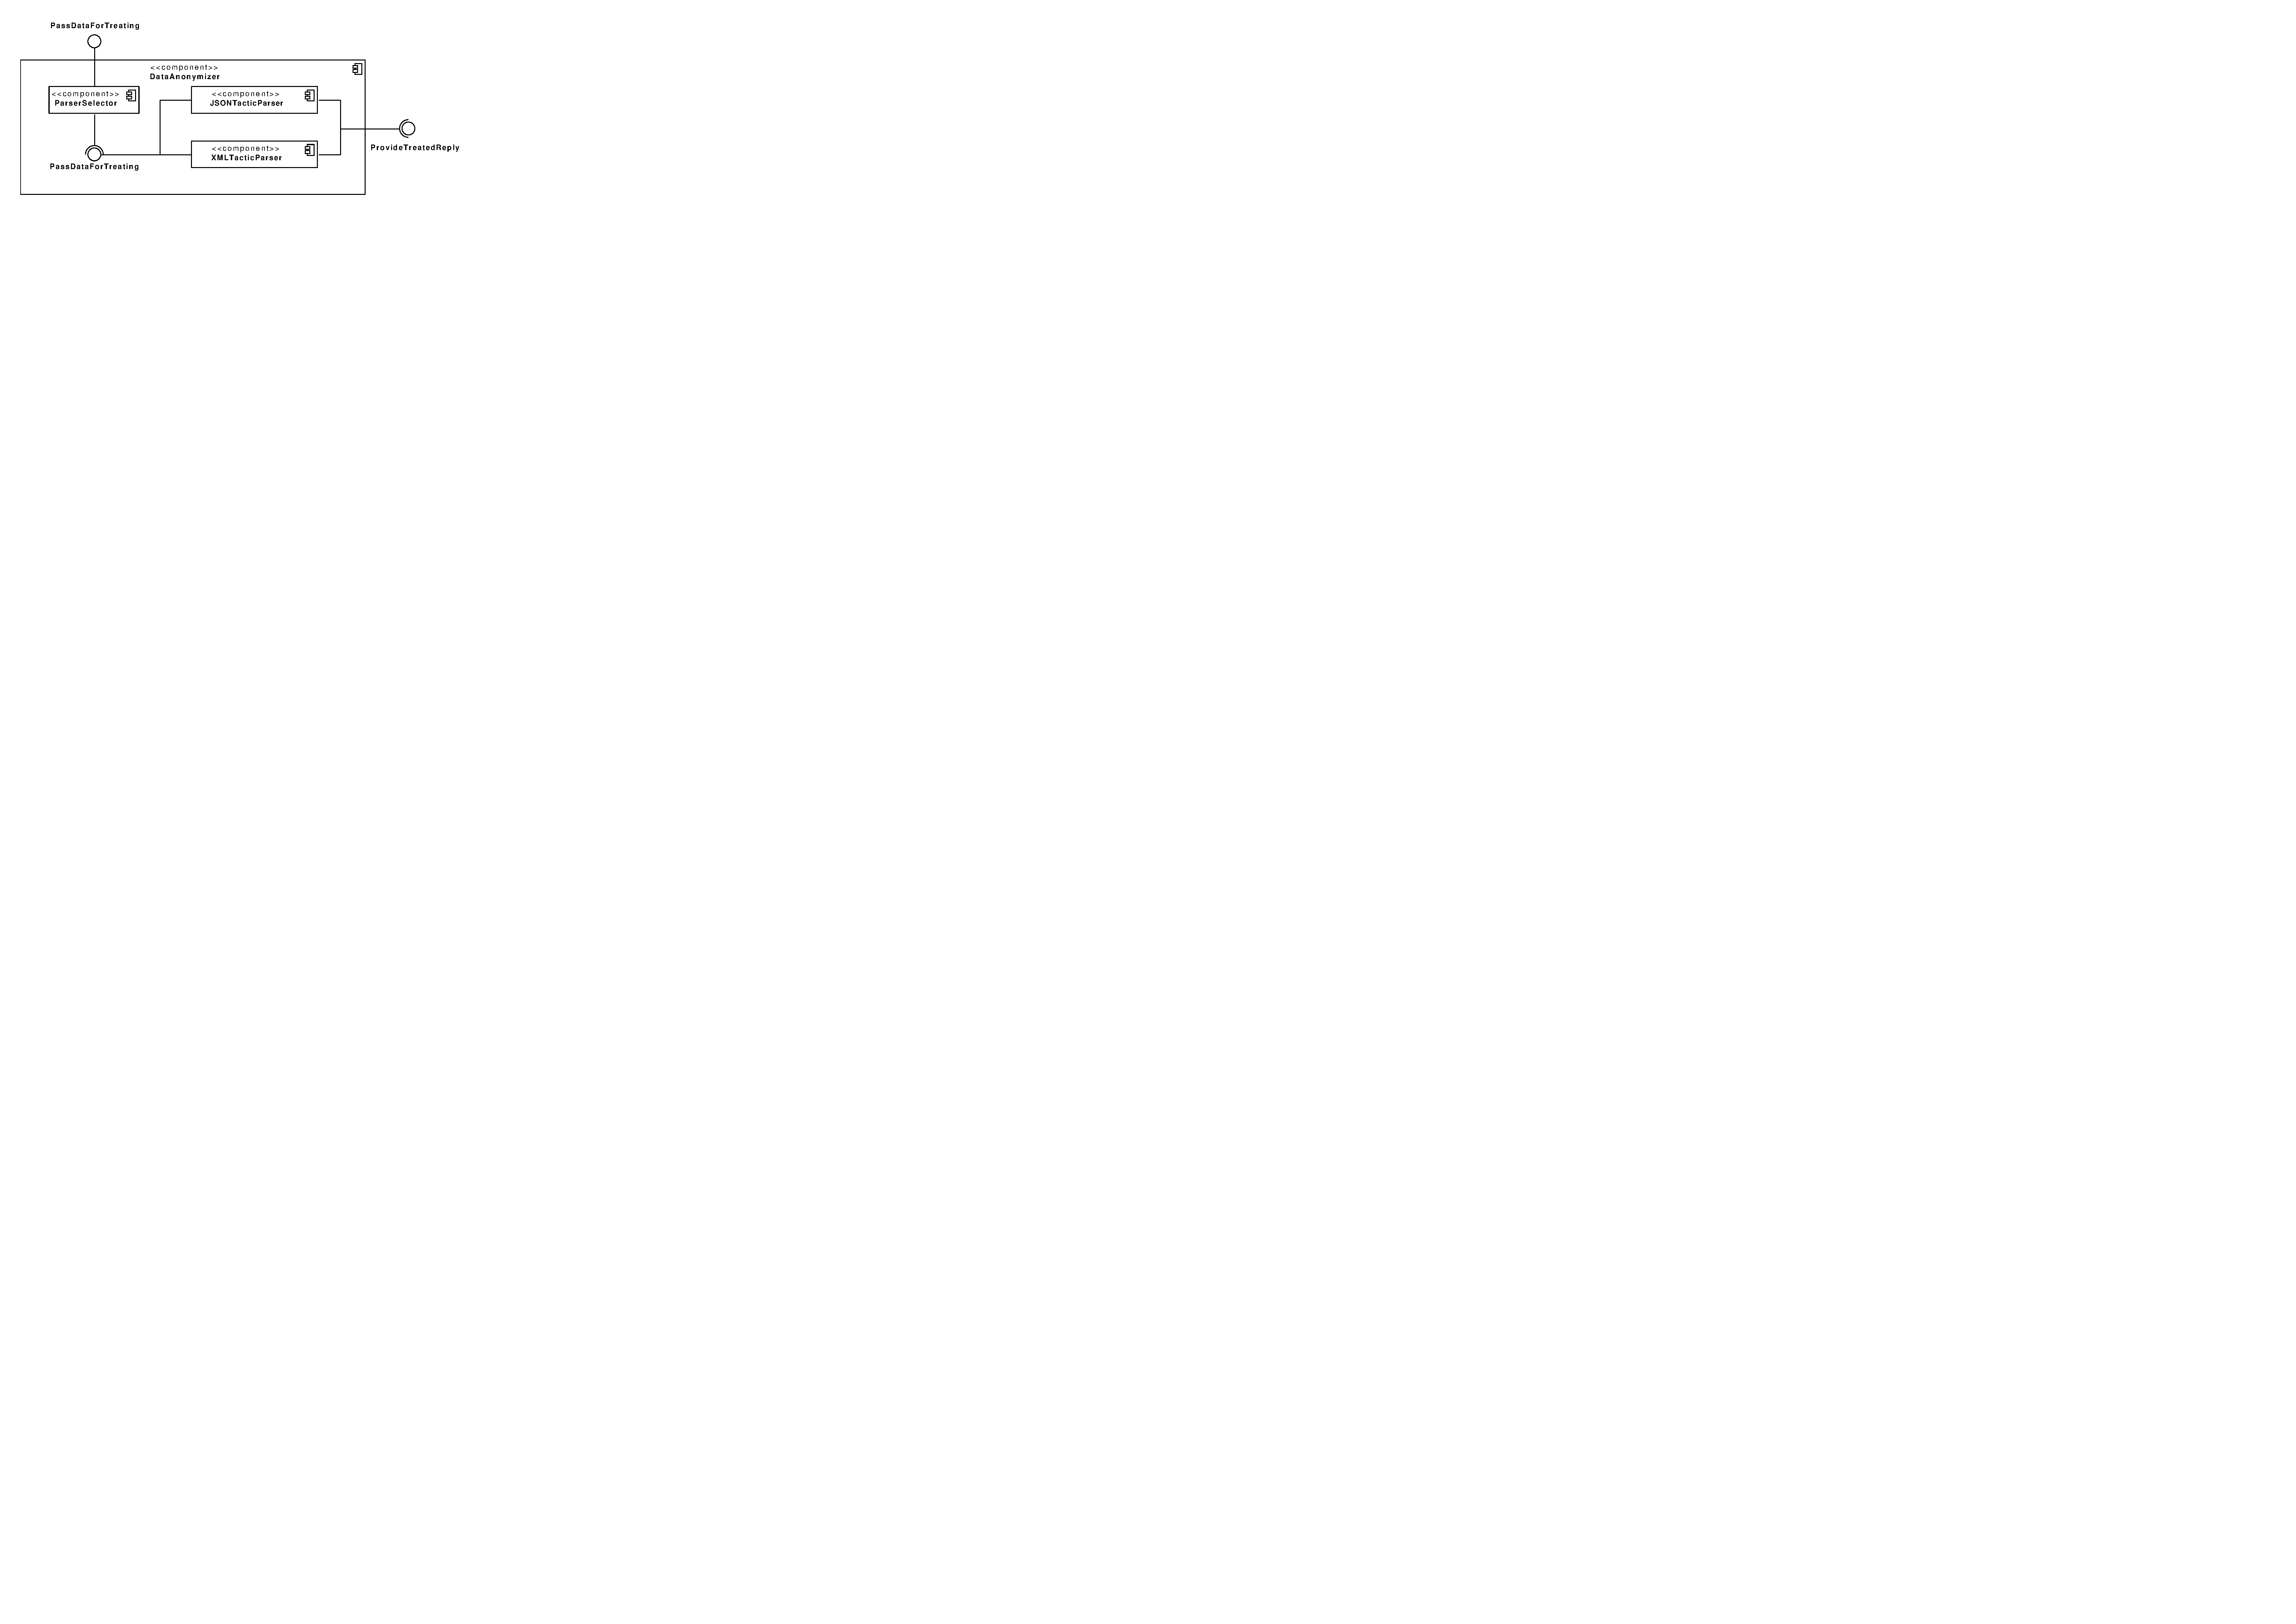
\includegraphics[width=\maxwidth{\textwidth}]{appendices/architecture/images/ComponentDiagram-DataAnonymizer-Component-Diagram.pdf}
  \caption[DataAnonymizer Component Diagram]{DataAnonymizer Component Diagram \label{diag:Component:DataAnonymizerComponentDiagram}}
\end{figure}

%%% DataTreatmentHandler Component Diagram (836.0x298.0)

\begin{figure}[!htp]
  \centering
  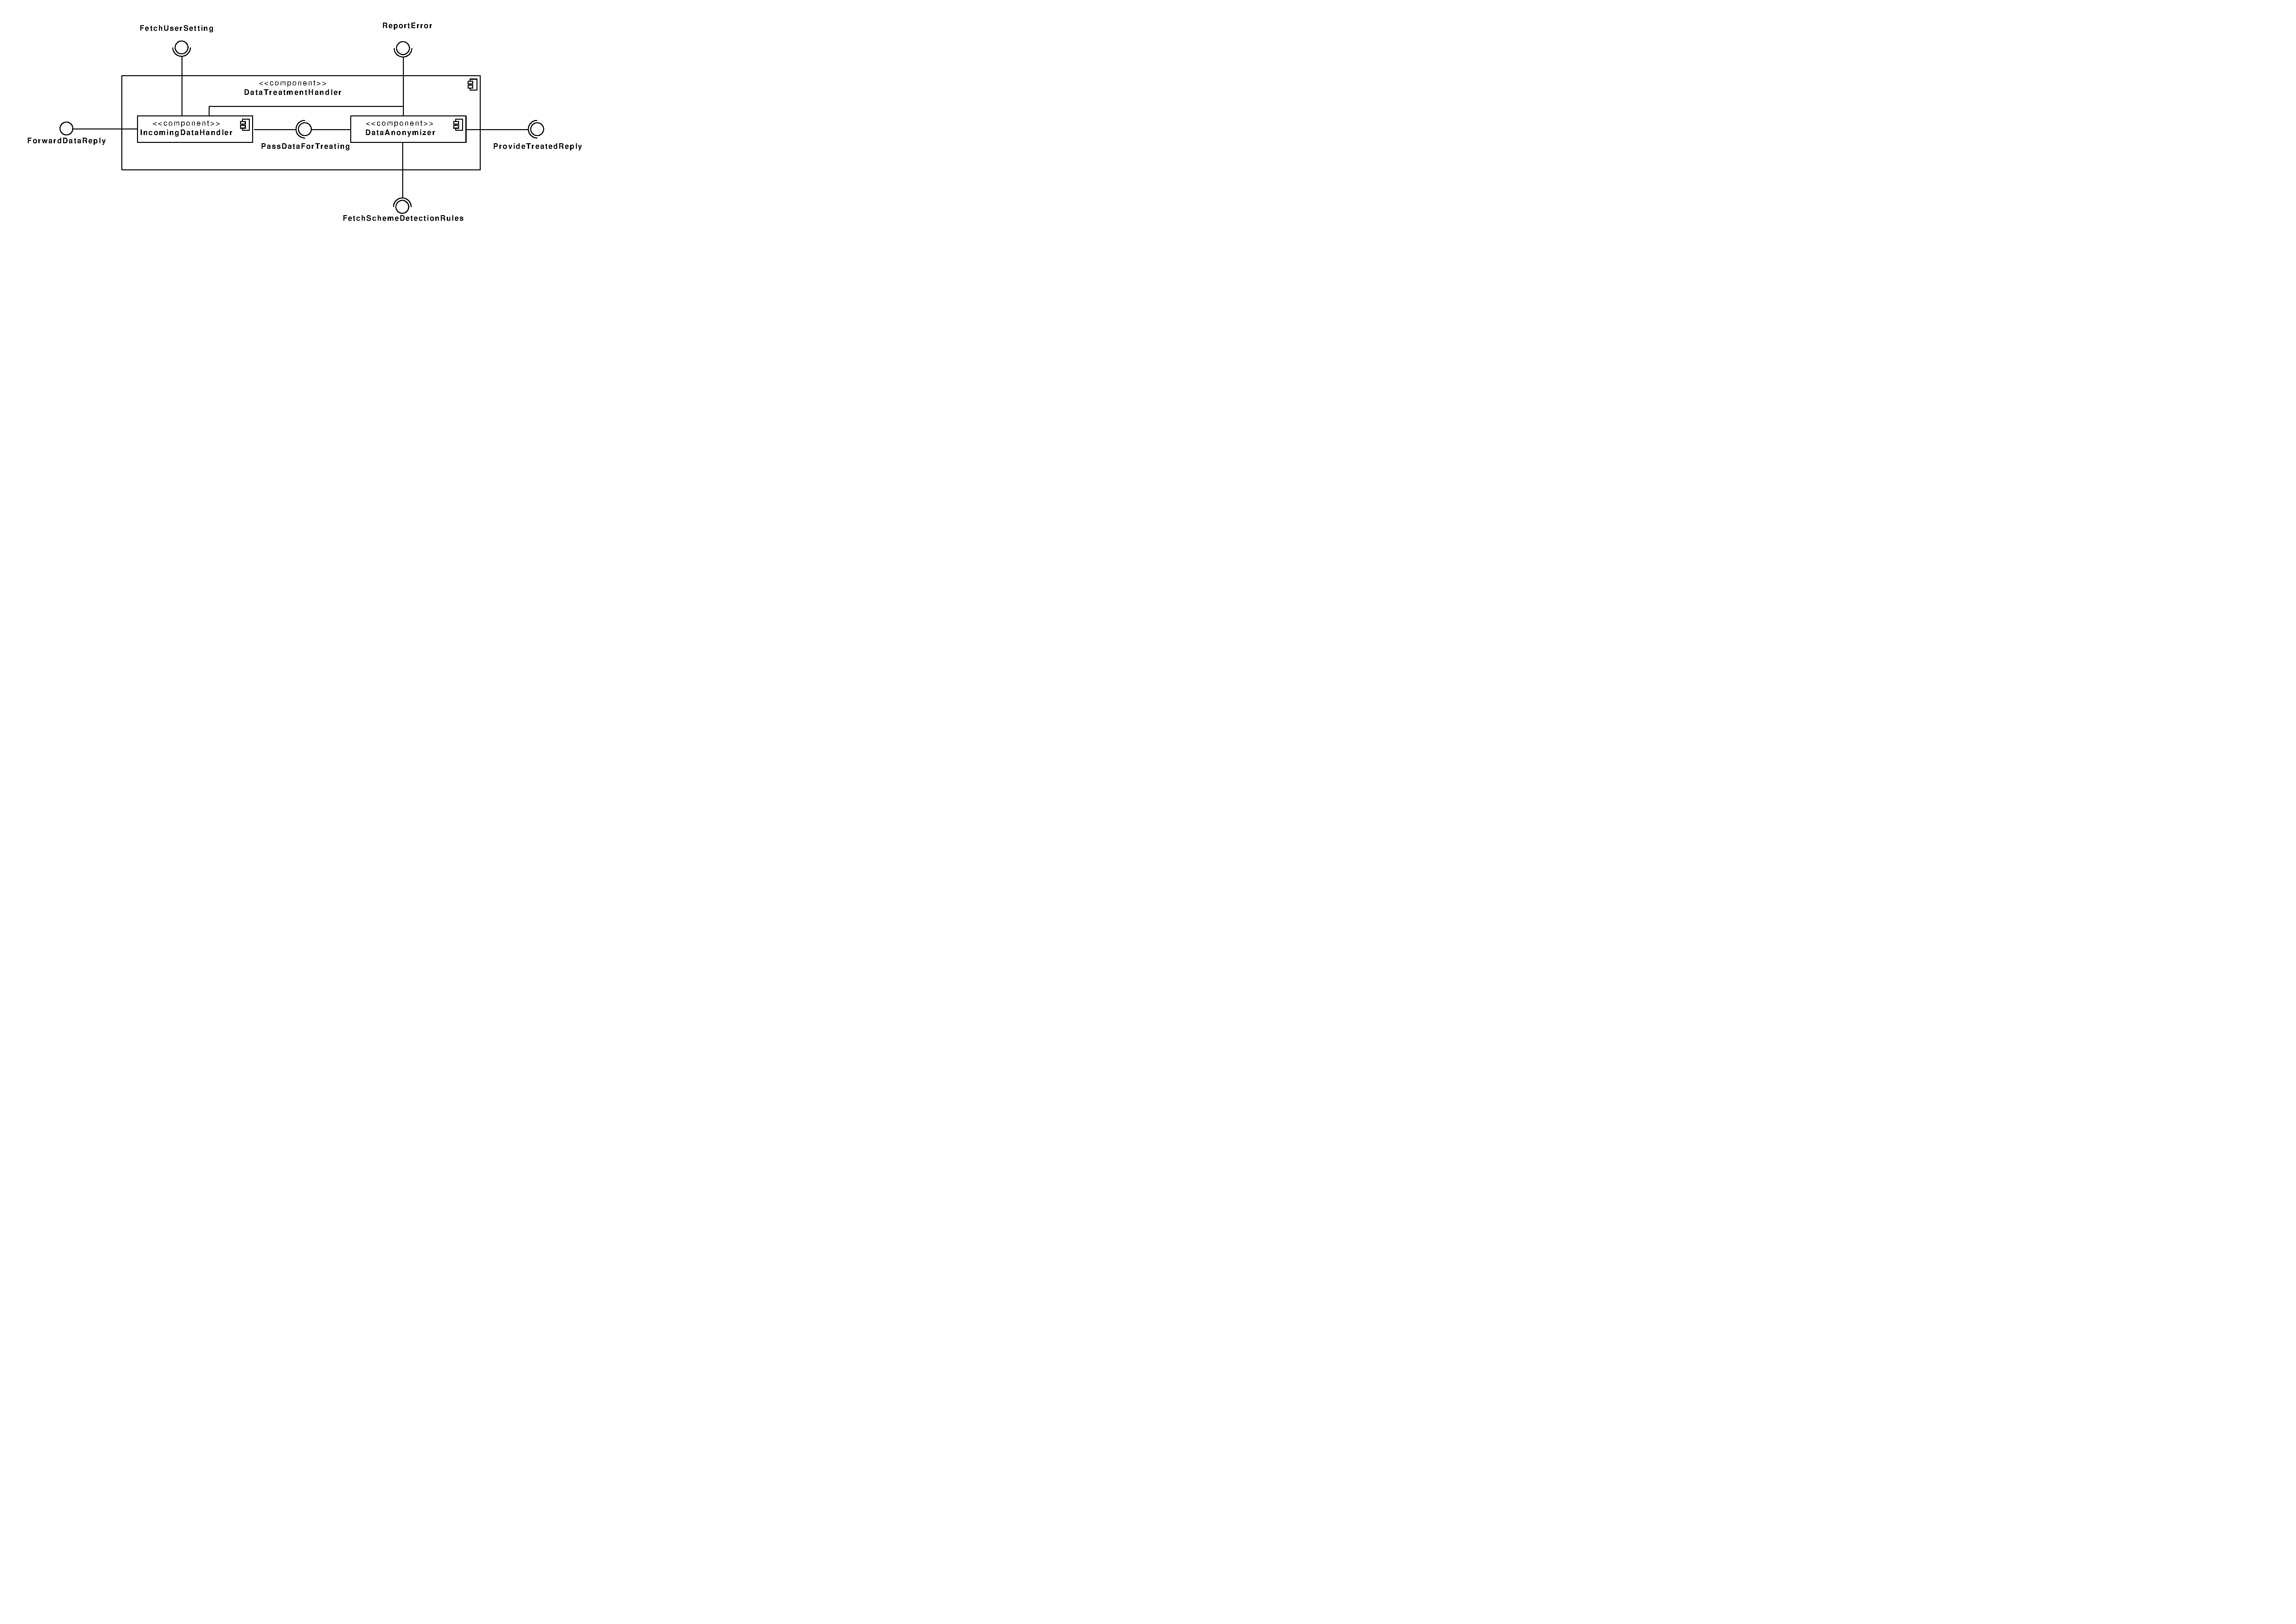
\includegraphics[width=\maxwidth{\textwidth}]{appendices/architecture/images/ComponentDiagram-DataTreatmentHandler-Component-Diagram.pdf}
  \caption[DataTreatmentHandler Component Diagram]{DataTreatmentHandler Component Diagram \label{diag:Component:DataTreatmentHandlerComponentDiagram}}
\end{figure}

%%% IncomingDataHandler Component Diagram (679.0x374.0)

\begin{figure}[!htp]
  \centering
  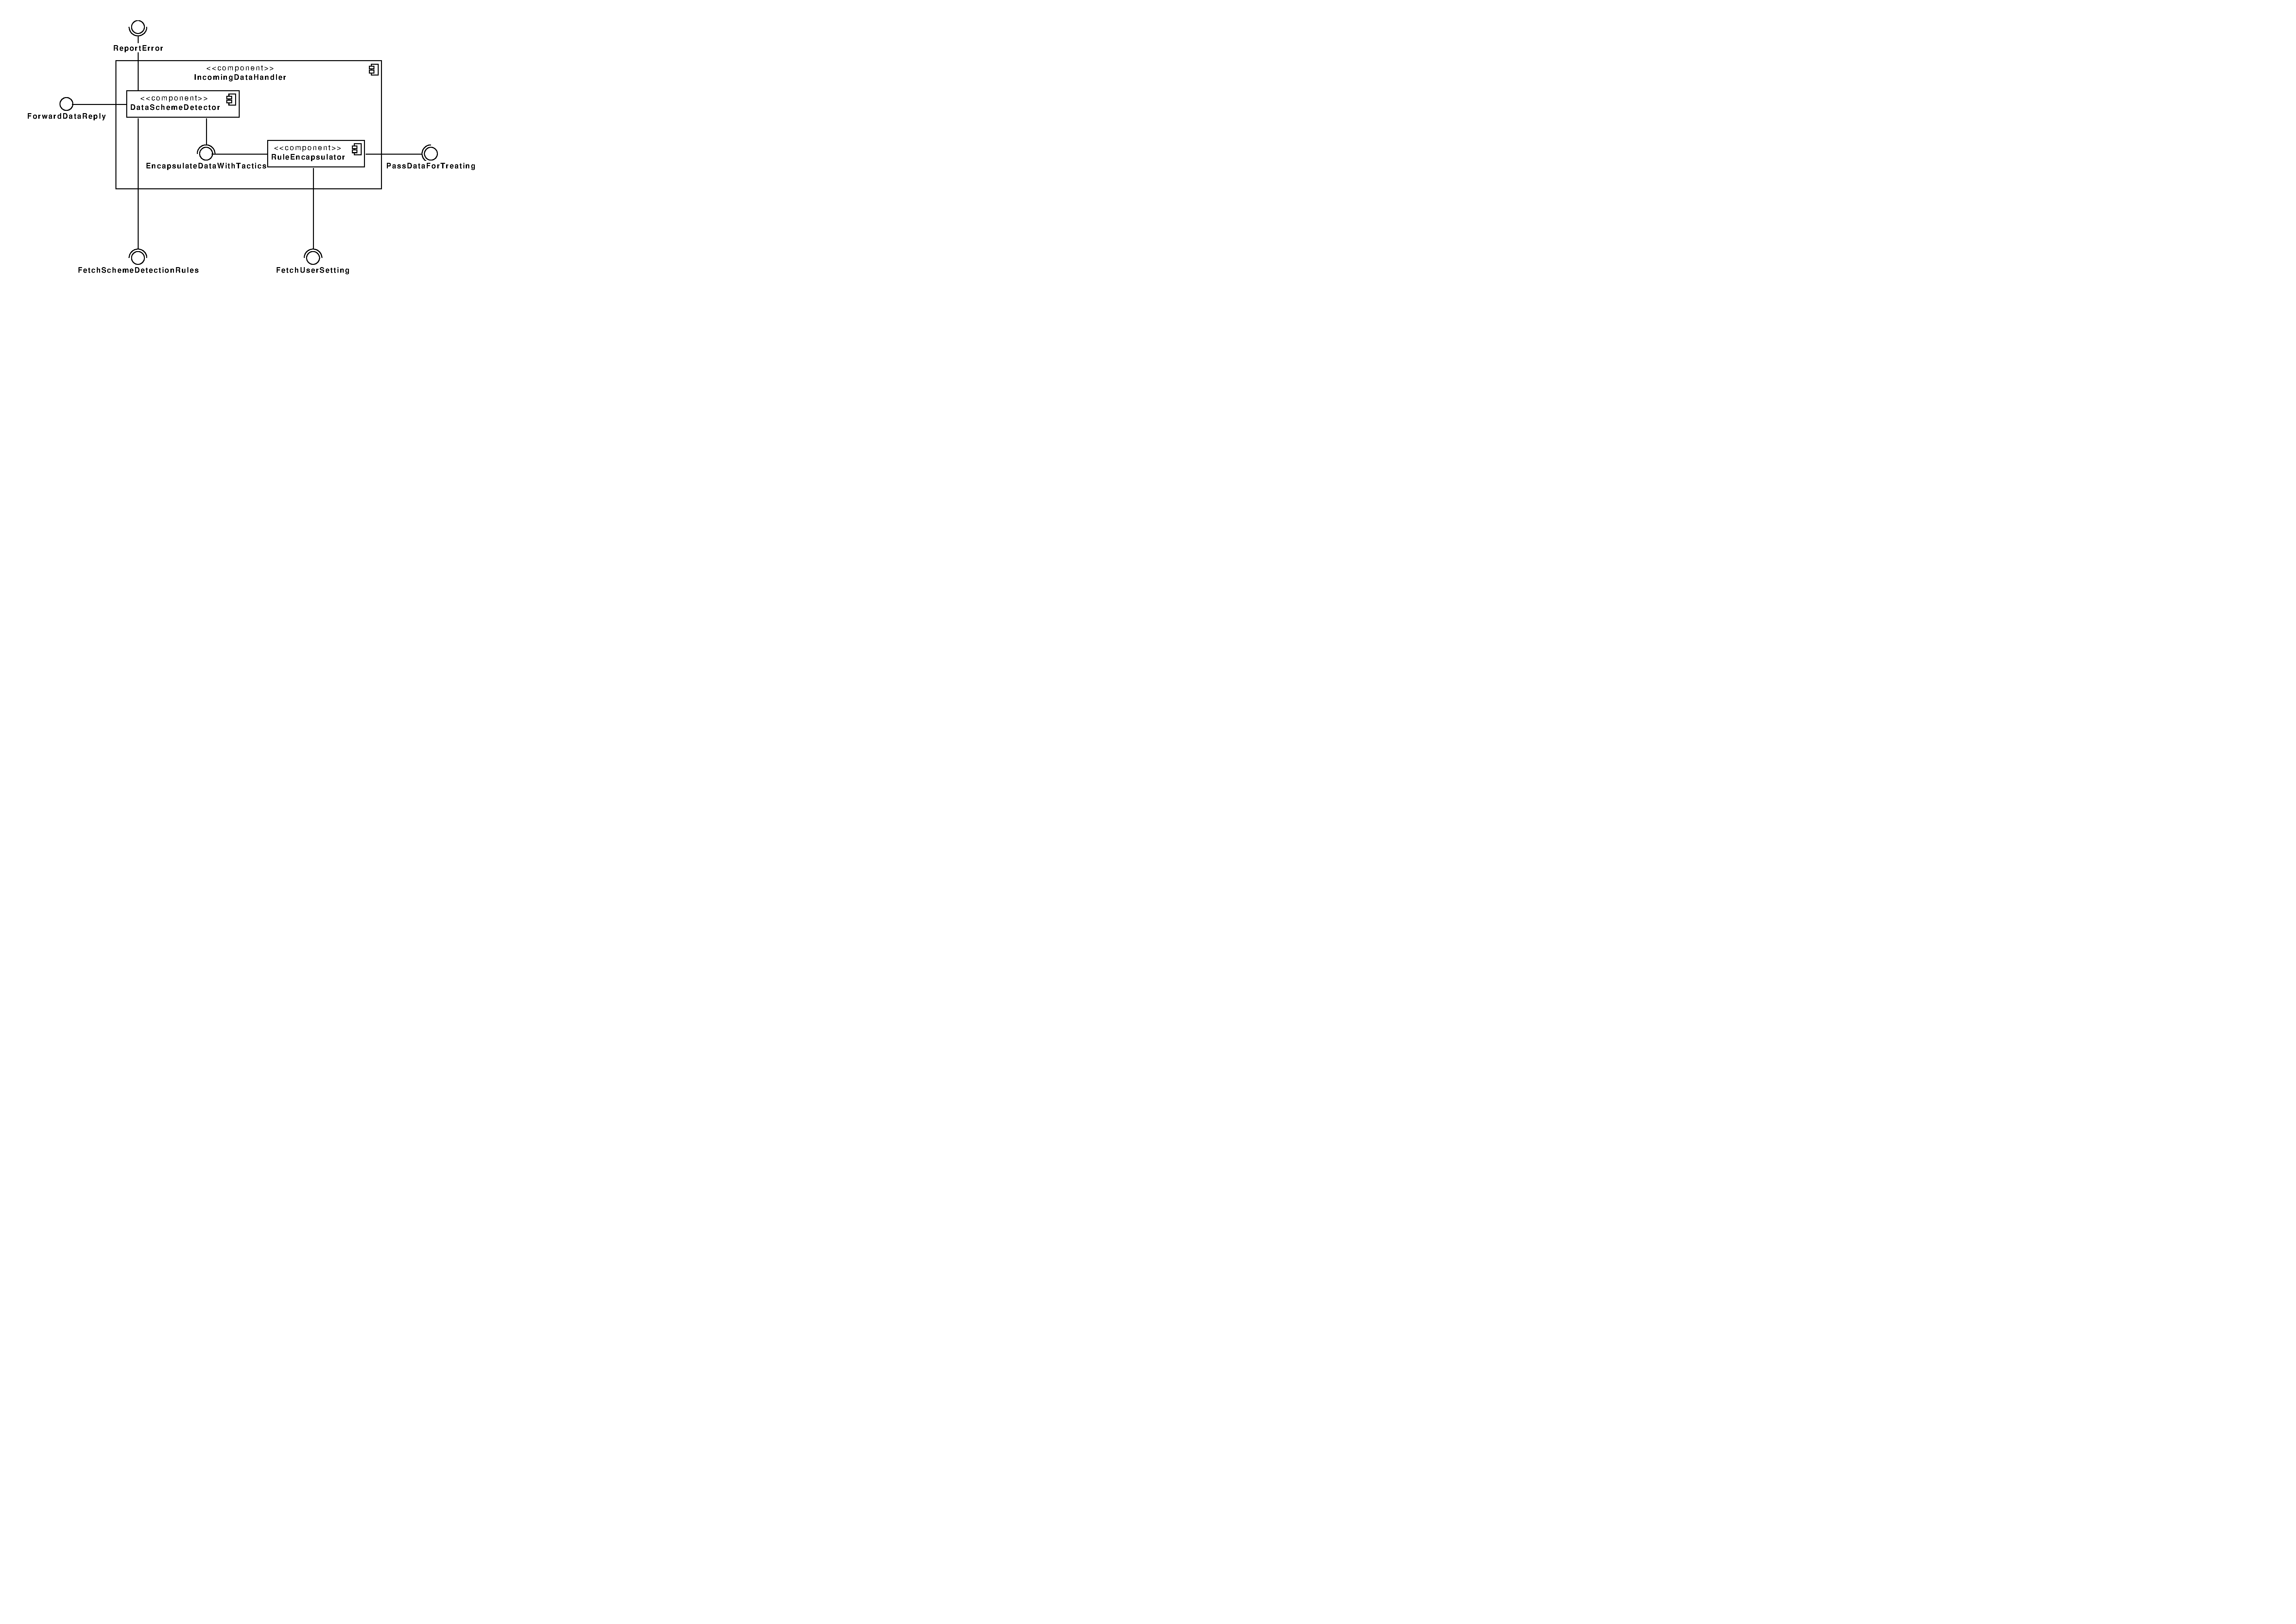
\includegraphics[width=\maxwidth{\textwidth}]{appendices/architecture/images/ComponentDiagram-IncomingDataHandler-Component-Diagram.pdf}
  \caption[IncomingDataHandler Component Diagram]{IncomingDataHandler Component Diagram \label{diag:Component:IncomingDataHandlerComponentDiagram}}
\end{figure}

%%% OutgoingHTTPHandler Component Diagram (833.0x316.0)

\begin{figure}[!htp]
  \centering
  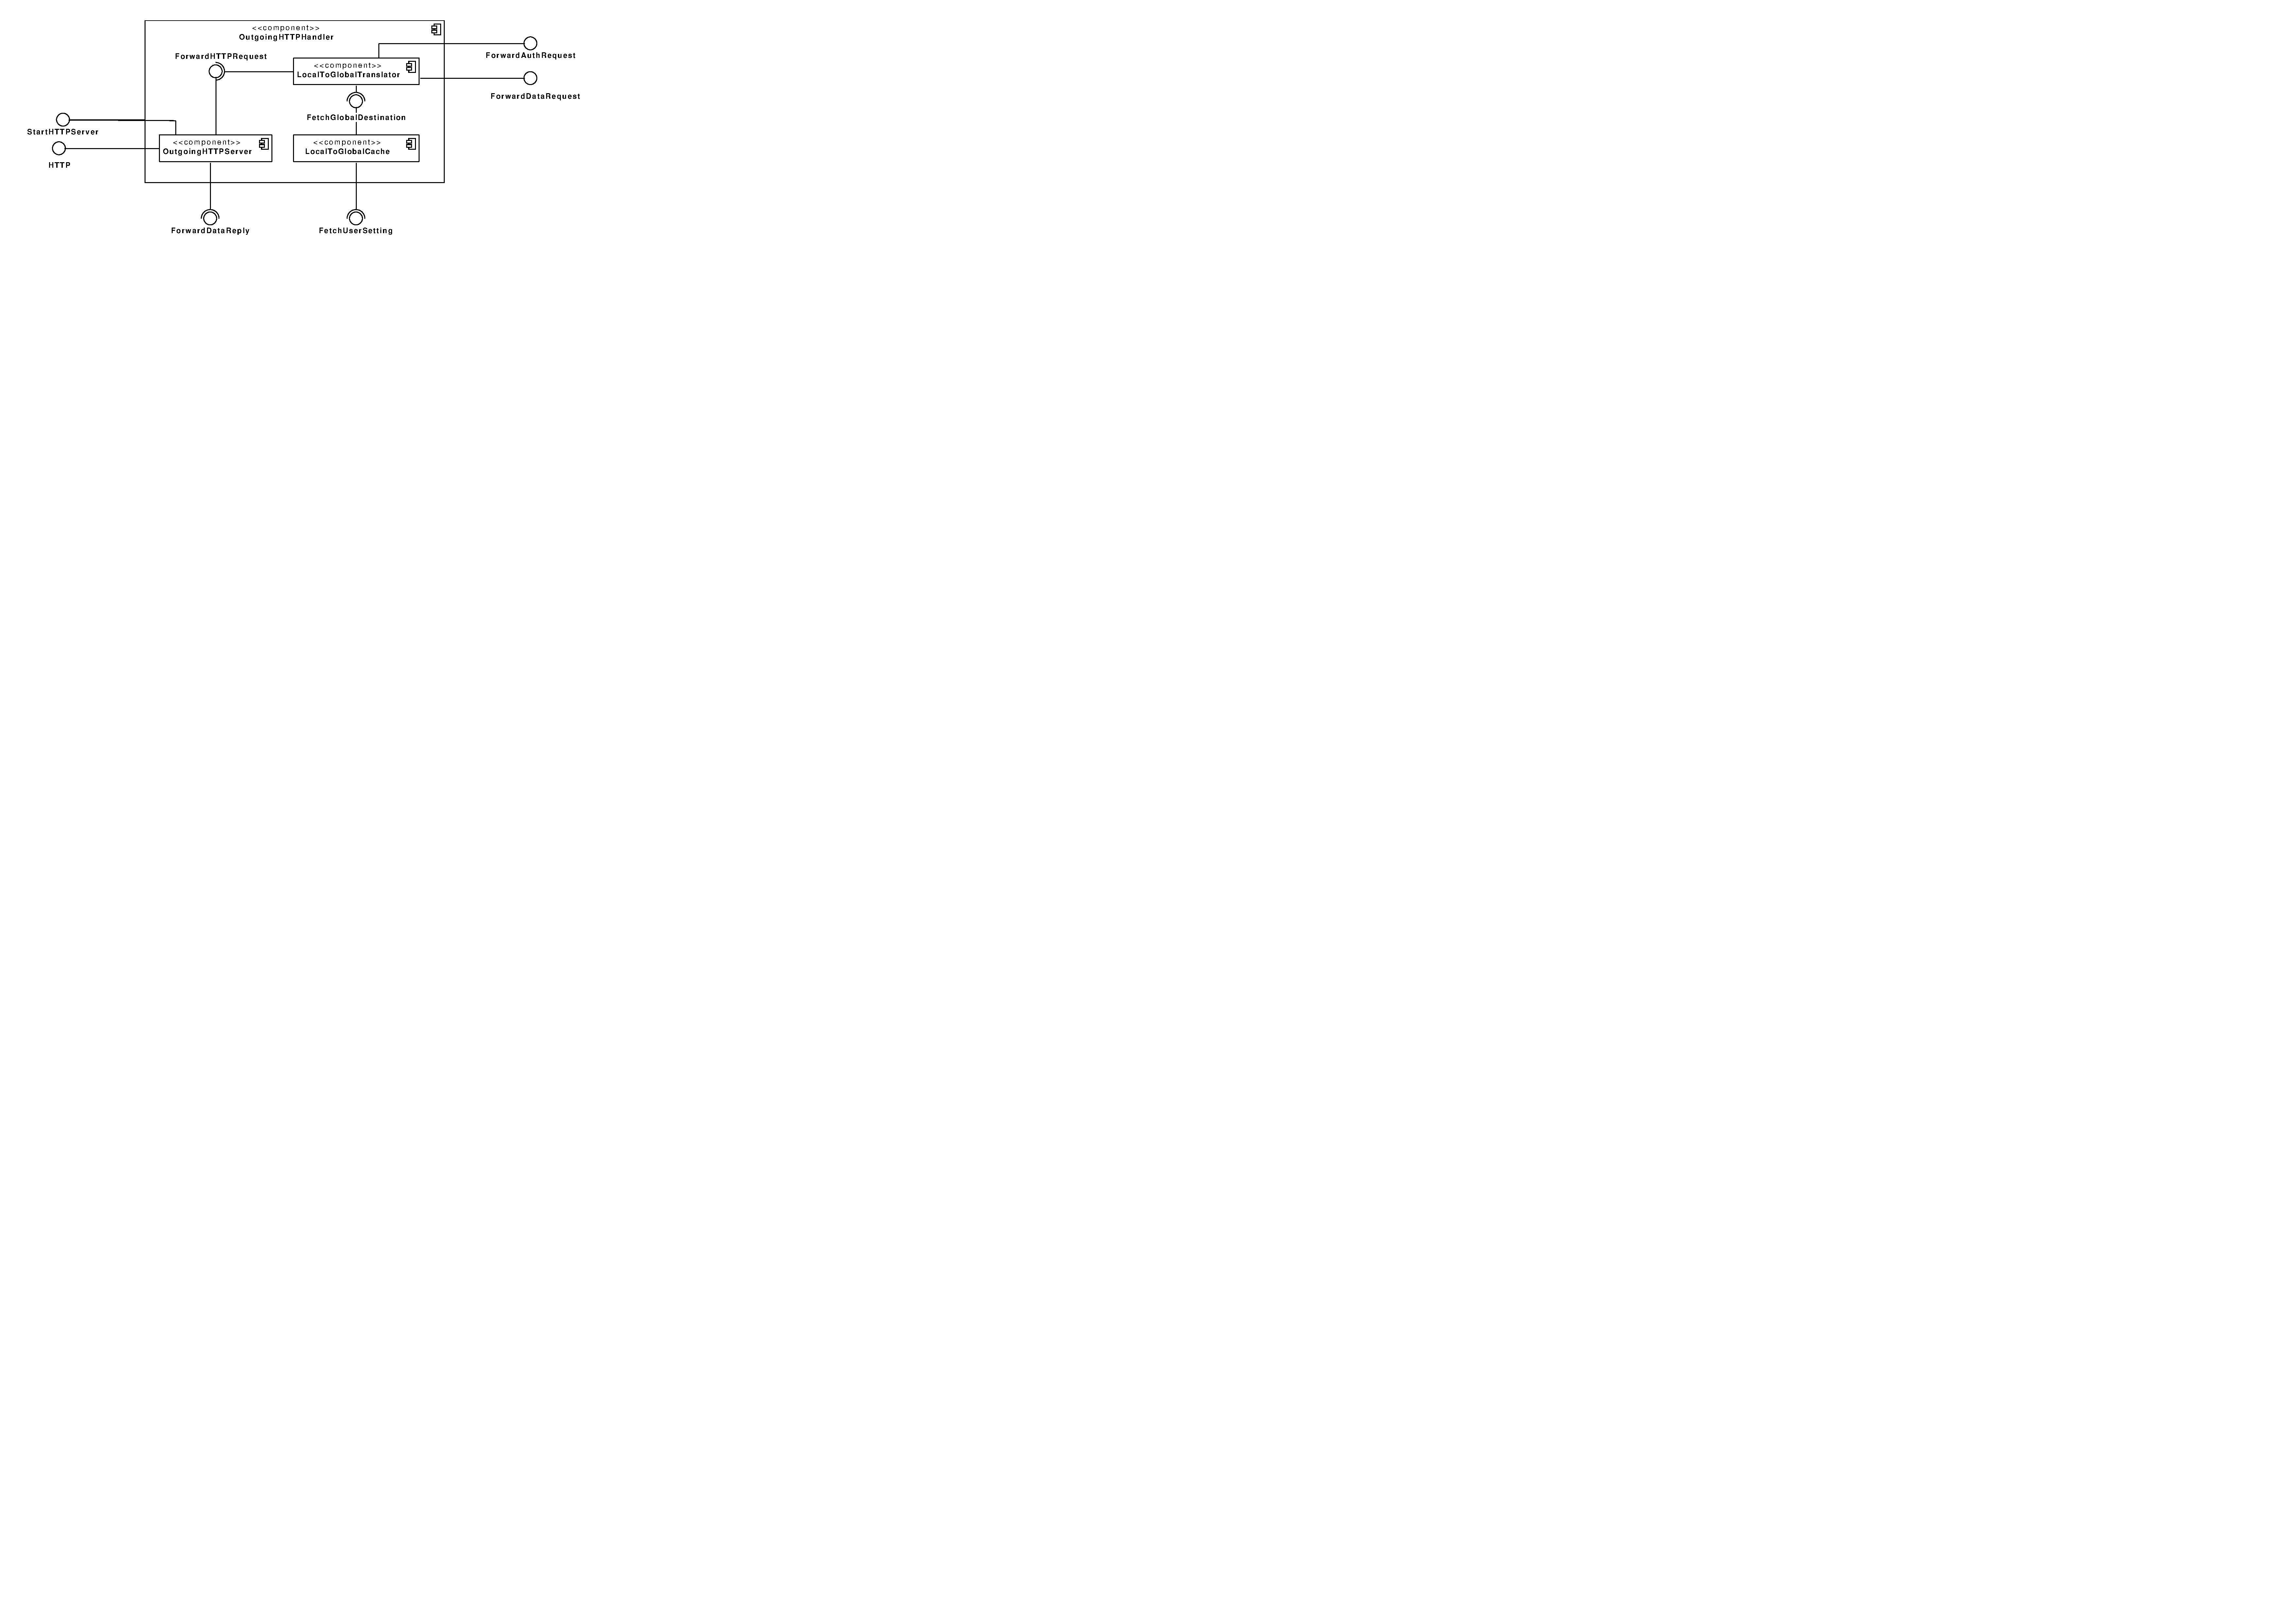
\includegraphics[width=\maxwidth{\textwidth}]{appendices/architecture/images/ComponentDiagram-OutgoingHTTPHandler-Component-Diagram.pdf}
  \caption[OutgoingHTTPHandler Component Diagram]{OutgoingHTTPHandler Component Diagram \label{diag:Component:OutgoingHTTPHandlerComponentDiagram}}
\end{figure}

%%% System Overview (927.0x393.0)

\begin{figure}[!htp]
  \centering
  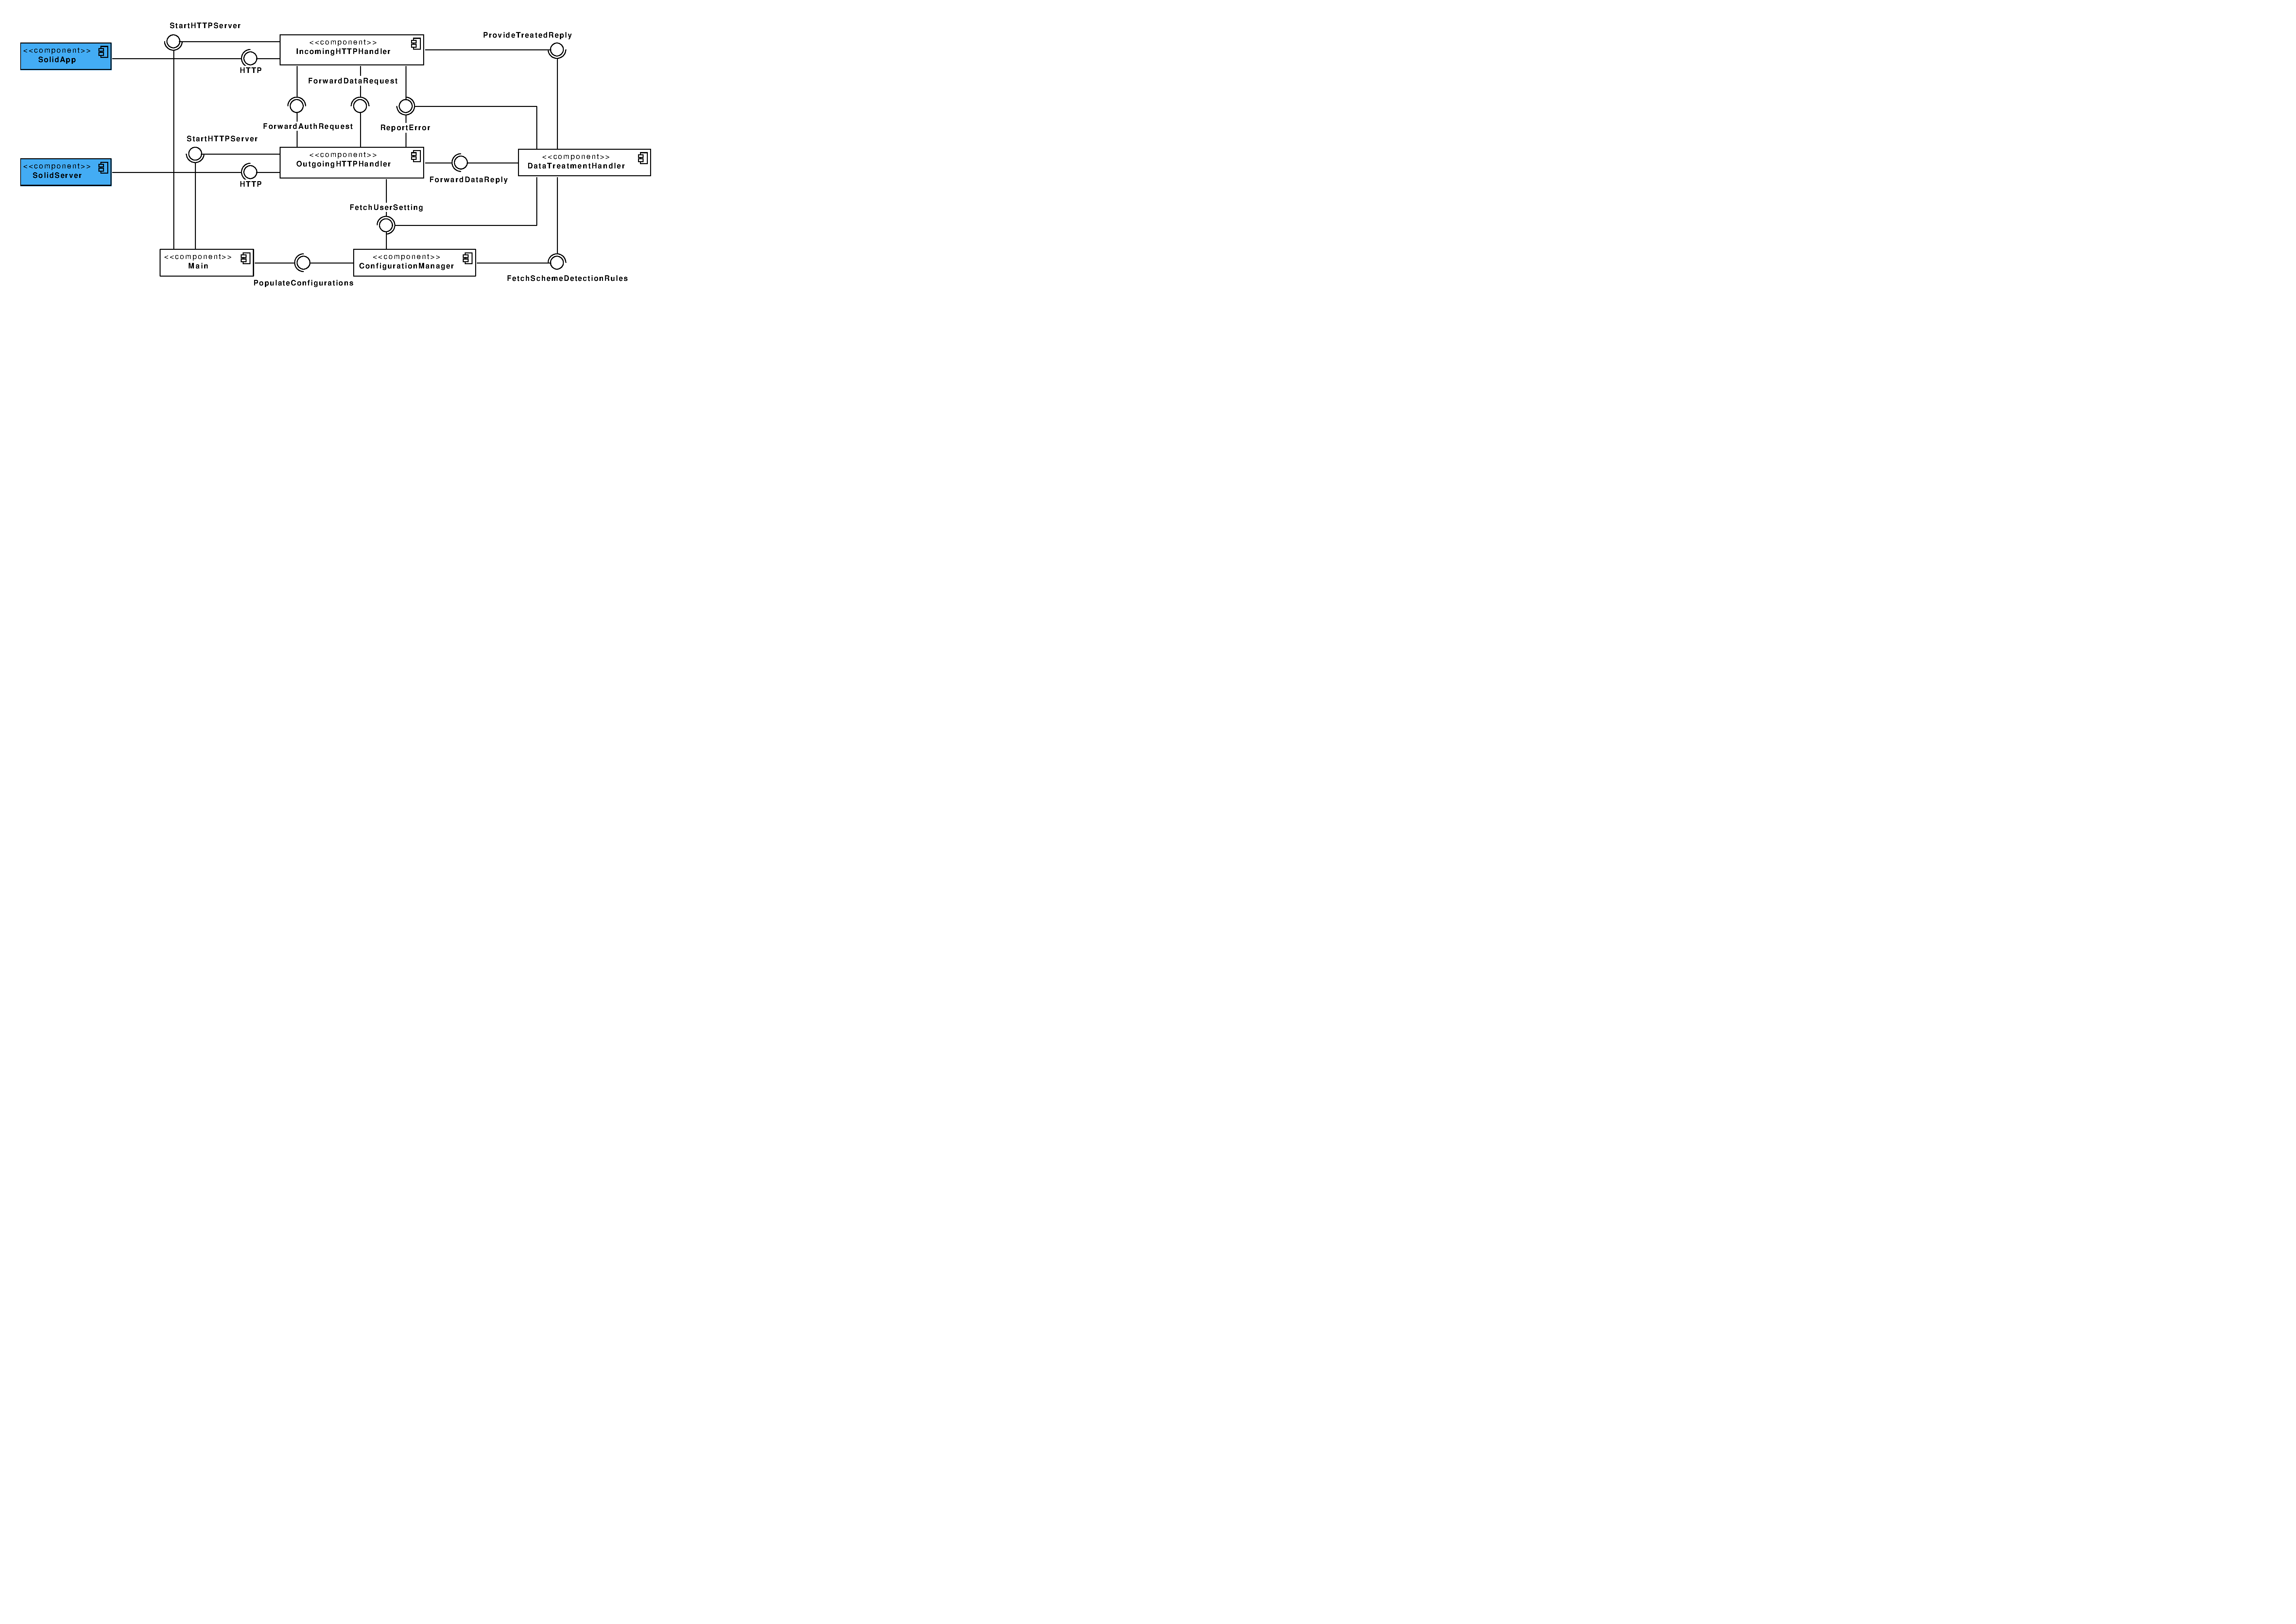
\includegraphics[width=\maxwidth{\textwidth}]{appendices/architecture/images/ComponentDiagram-System-Overview.pdf}
  \caption[System Overview]{System Overview \label{diag:Component:SystemOverview}}
\end{figure}



%%%%%%%%%%%%%%%%%%%%%%%%%%%%%%%%%%%%%%%%%%%%%%%%%%%%
%%% DEPLOYMENT
%%%%%%%%%%%%%%%%%%%%%%%%%%%%%%%%%%%%%%%%%%%%%%%%%%%%
\chapter{Deployment view (UML Deployment Diagram)}
\minilof{}




%%% Deployment Diagram (953.0x282.0)

\begin{figure}[!htp]
  \centering
  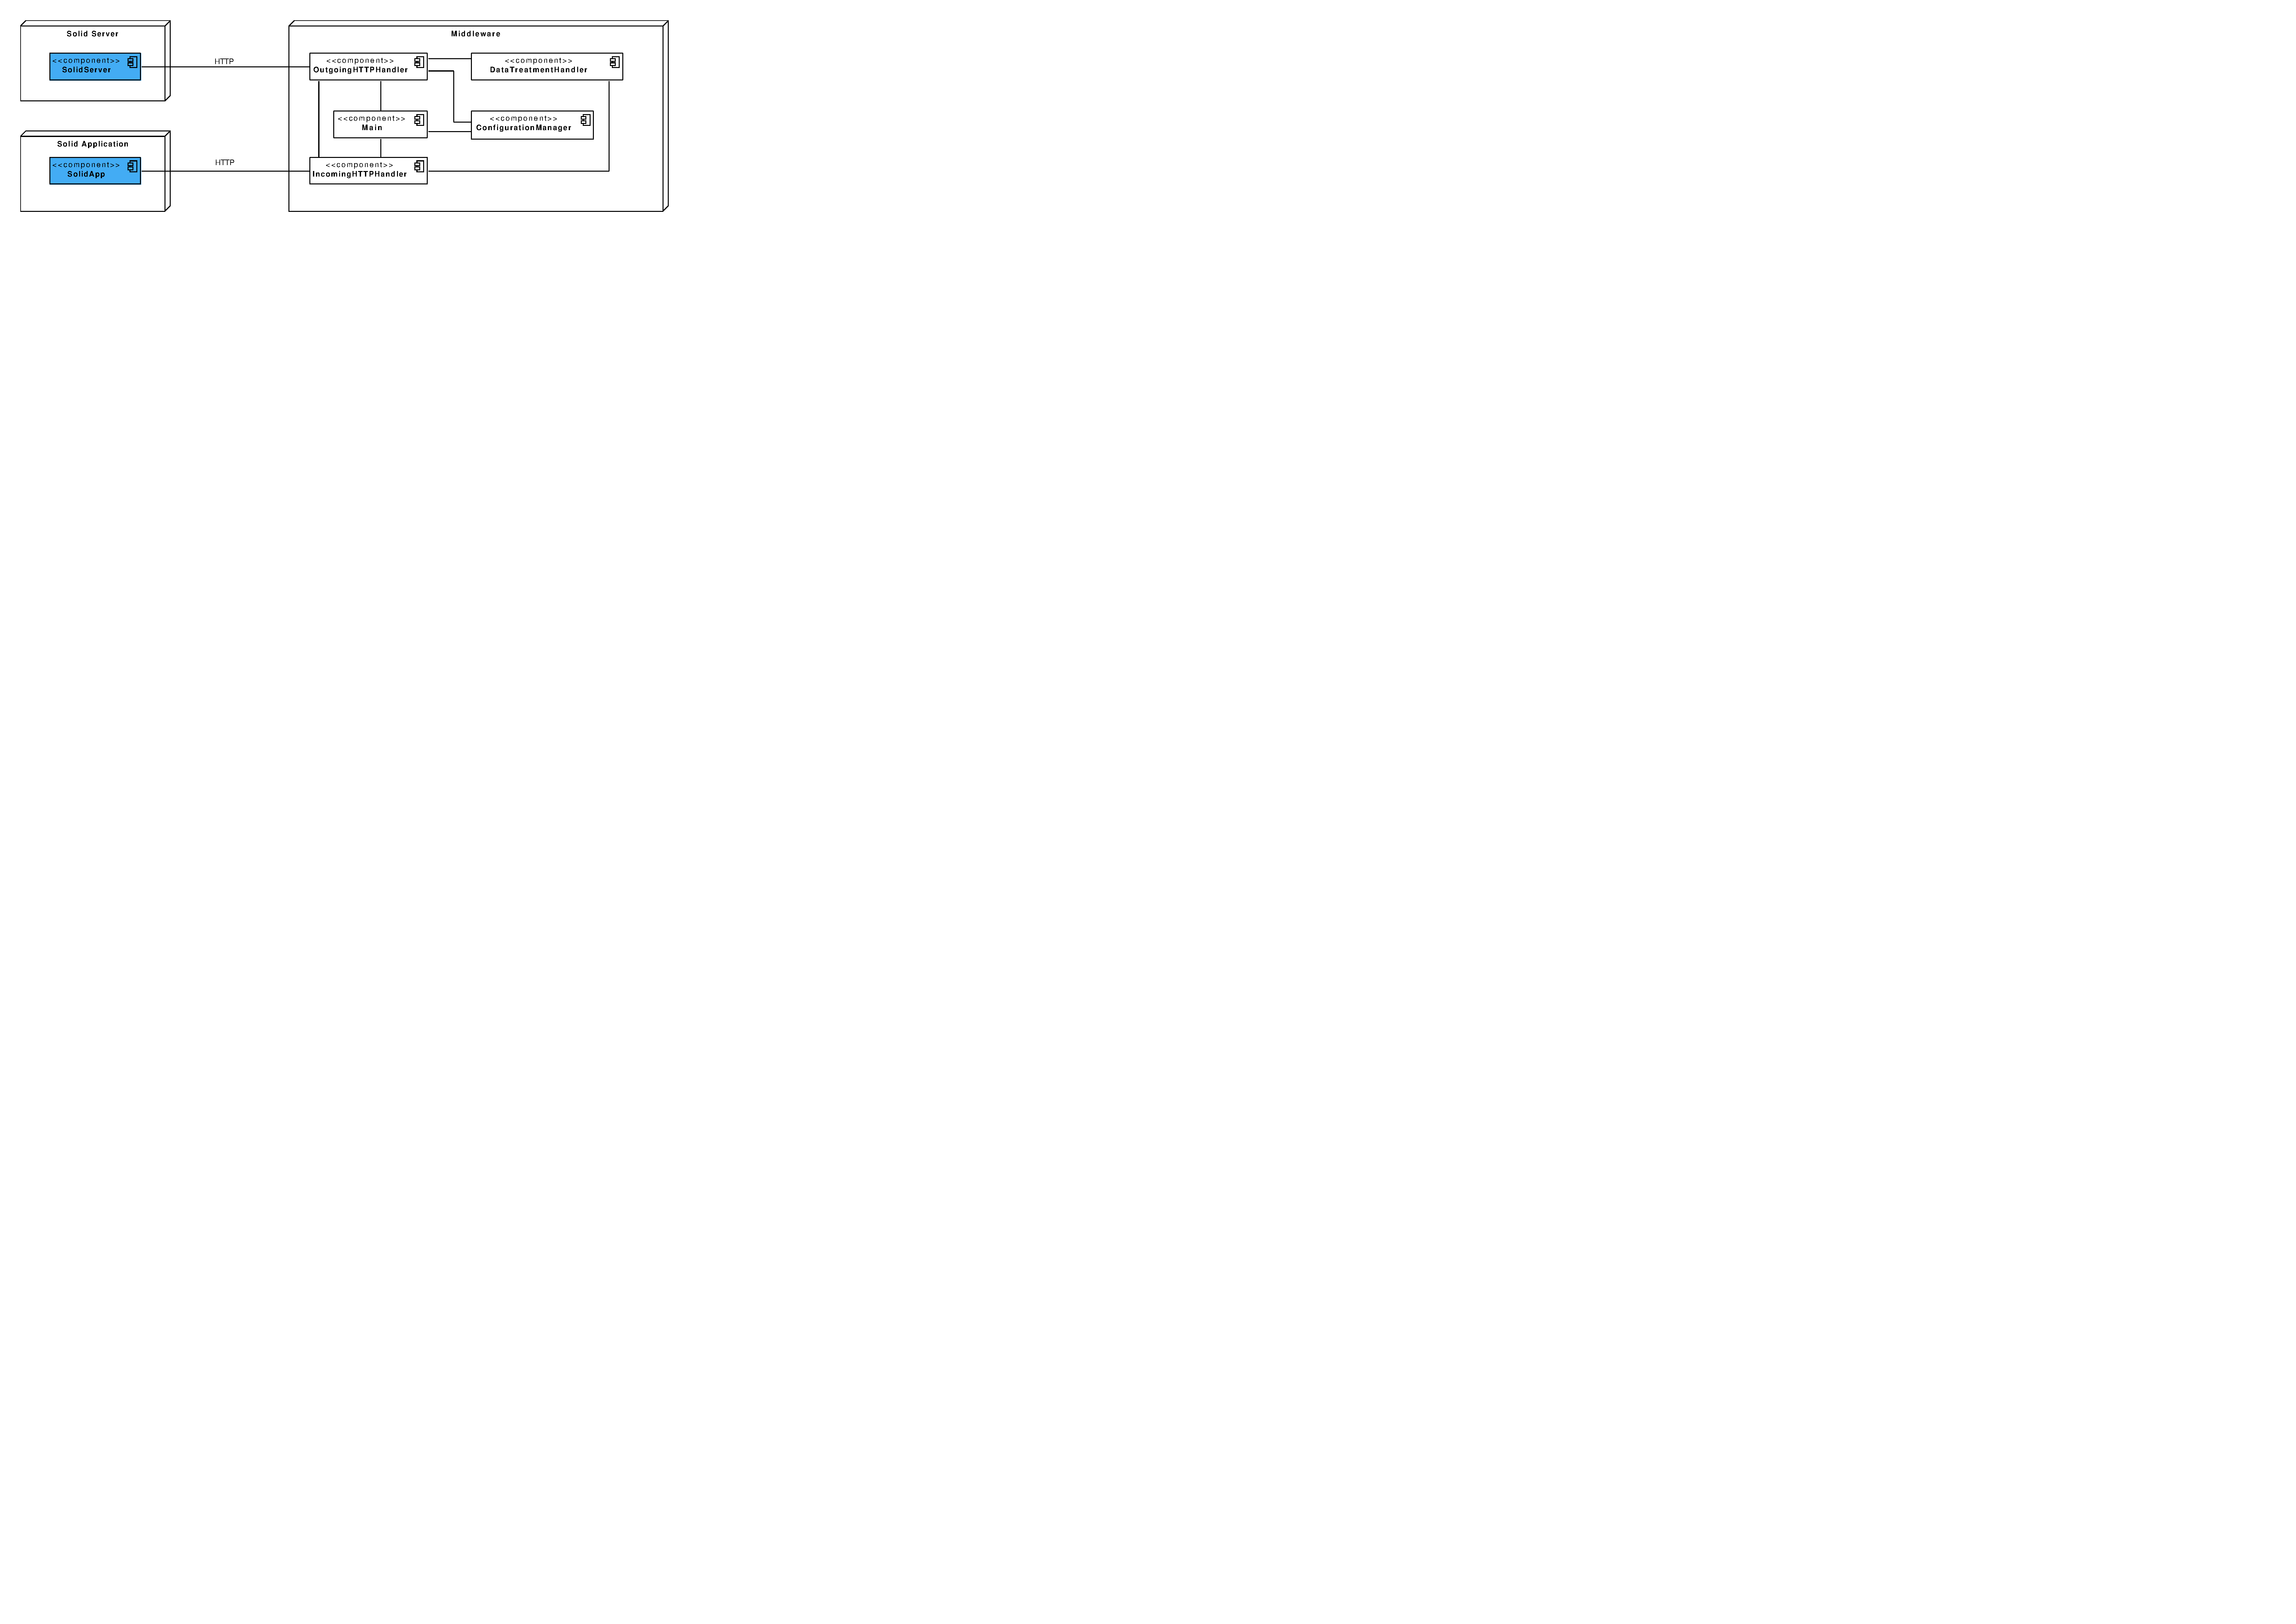
\includegraphics[width=\maxwidth{\textwidth}]{appendices/architecture/images/DeploymentDiagram-Deployment-Diagram.pdf}
  \caption[Deployment Diagram]{Deployment Diagram \label{diag:Deployment:DeploymentDiagram}}
\end{figure}



%%%%%%%%%%%%%%%%%%%%%%%%%%%%%%%%%%%%%%%%%%%%%%%%%%%%
%%% SEQUENCE
%%%%%%%%%%%%%%%%%%%%%%%%%%%%%%%%%%%%%%%%%%%%%%%%%%%%
\chapter{Process View (UML Sequence Diagram)}
\minilof{}


%%% Data flow (1305.0x406.0)

\begin{figure}[!htp]
  \centering
  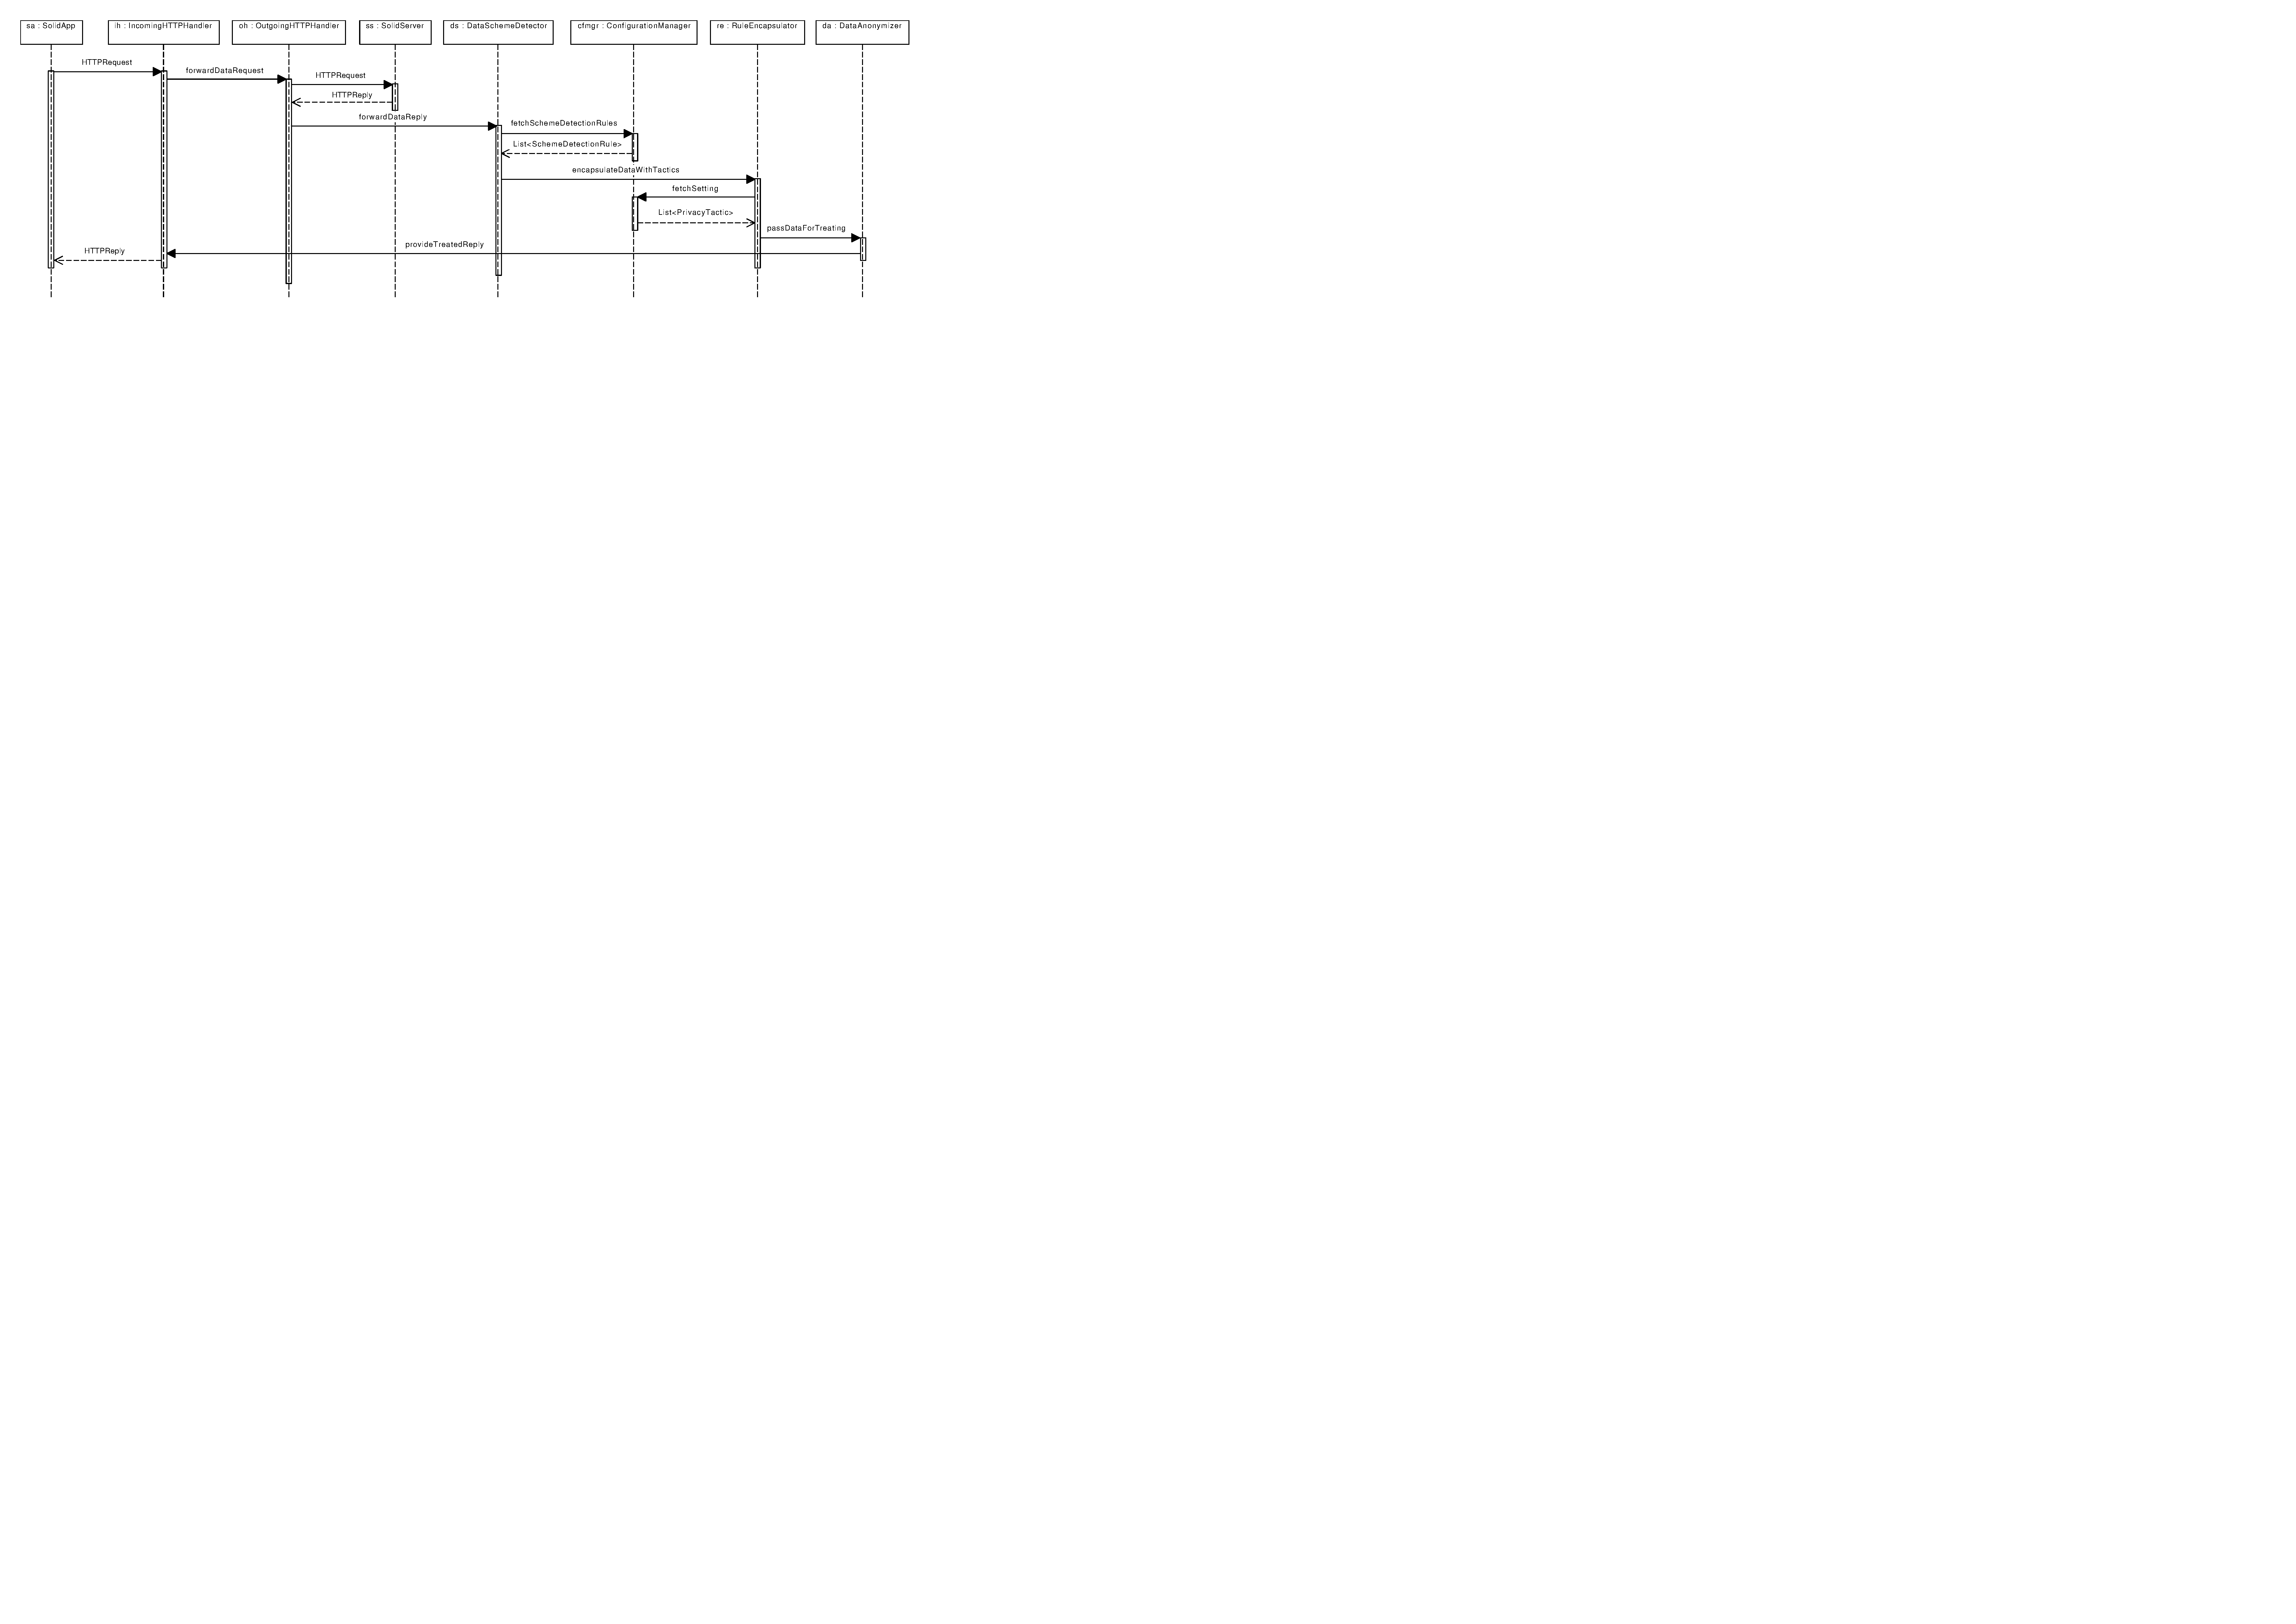
\includegraphics[width=\maxwidth{\textwidth}]{appendices/architecture/images/InteractionDiagram-Data-flow.pdf}
  \caption[Data flow]{Data flow \label{diag:Interaction:Dataflow}}
\end{figure}

%%% element catalog, generated on Sun Nov 28 22:49:53 CET 2021

%%% WARNING %%%
%%% This file was automatically generated by SAPlugin,
%%% and will be overwritten next time.

\chapter{Element catalog}\label{sec:catalog}
% COMPONENTS
\section{Components}\label{sec:components}
\subsection{ConfigurationManager}\label{comp:ComponentsConfigurationManager}
	\begin{description}[noitemsep,nolistsep]
		\item[Responsibility:]~The \vpett{\nameref{comp:ComponentsConfigurationManager}} component is responsible for storing all configurable settings, such as:
* The URL of the user's pod to connect to
* The URL the middleware should be deployed to
* A list of supported data schemes, and for each data scheme the settings as to which privacy level maps to which transformations
* Which privacy level should be applied (either by default, or for specific data schemes)
		\item[Super-components:]~None
		\item[Sub-components:]~None
		\item[Provided interfaces:]~\iconprovided{}~\vpett{\nameref{int:InterfacesFetchSchemeDetectionRules}}, \iconprovided{}~\vpett{\nameref{int:InterfacesFetchUserSetting}}, \iconprovided{}~\vpett{\nameref{int:InterfacesPopulateConfigurations}}
		\item[Required interfaces:]~None
		\item[Deployed on:]~\faSquareO~\vpett{\nameref{node:DeploymentMiddleware}}
		\item[Visible on diagrams:]~\cref{diag:Component:SystemOverview,diag:Deployment:DeploymentDiagram,diag:Interaction:Dataflow}		
	\end{description}

\subsection{DataAnonymizer}\label{comp:ComponentsDataTreatmentHandlerDataAnonymizer}
	\begin{description}[noitemsep,nolistsep]
		\item[Responsibility:]~The \vpett{\nameref{comp:ComponentsDataTreatmentHandlerDataAnonymizer}} is the main component responsible for taking in raw data (of which the scheme has already been detected, and the tactics necessary to be performed have been added to the data). It then performs all the required tactics on the data, using different components based on the content-representation of the data.
When no scheme is detected, a "\ref{data:ExceptionsNoMatchingSchemeException}" is thrown.
		\item[Super-components:]~\iconcomponent{}~\vpett{\nameref{comp:ComponentsDataTreatmentHandler}}
		\item[Sub-components:]~\iconcomponent{}~\vpett{\nameref{comp:ComponentsDataTreatmentHandlerDataAnonymizerJSONTacticParser}}, \iconcomponent{}~\vpett{\nameref{comp:ComponentsDataTreatmentHandlerDataAnonymizerXMLTacticParser}}, \iconcomponent{}~\vpett{\nameref{comp:ComponentsDataTreatmentHandlerDataAnonymizerParserSelector}}
		\item[Provided interfaces:]~\iconprovided{}~\vpett{\nameref{int:InterfacesPassDataForTreating}}
		\item[Required interfaces:]~\iconrequired{}~\vpett{\nameref{int:InterfacesFetchSchemeDetectionRules}}, \iconrequired{}~\vpett{\nameref{int:InterfacesProvideTreatedReply}}, \iconrequired{}~\vpett{\nameref{int:InterfacesReportError}}
		\item[Deployed on:]~\faSquareO~\vpett{\nameref{node:DeploymentMiddleware}}
		\item[Visible on diagrams:]~\cref{diag:Component:DataAnonymizerComponentDiagram,diag:Component:DataTreatmentHandlerComponentDiagram,diag:Interaction:Dataflow}		
	\end{description}

\subsection{DataSchemeDetector}\label{comp:ComponentsDataTreatmentHandlerIncomingDataHandlerDataSchemeDetector}
	\begin{description}[noitemsep,nolistsep]
		\item[Responsibility:]~The \vpett{\nameref{comp:ComponentsDataTreatmentHandlerIncomingDataHandlerDataSchemeDetector}} is the component responsible for taking in raw data, and then (using a set of SchemeDetectionRules), determining which scheme the data uses.
		\item[Super-components:]~\iconcomponent{}~\vpett{\nameref{comp:ComponentsDataTreatmentHandlerIncomingDataHandler}} $\triangleright$ \iconcomponent{}~\vpett{\nameref{comp:ComponentsDataTreatmentHandler}}
		\item[Sub-components:]~None
		\item[Provided interfaces:]~\iconprovided{}~\vpett{\nameref{int:InterfacesForwardDataReply}}, \iconprovided{}~\vpett{\nameref{int:InterfacesPassDataForTreating}}
		\item[Required interfaces:]~\iconrequired{}~\vpett{\nameref{int:InterfacesEncapsulateDataWithTactics}}, \iconrequired{}~\vpett{\nameref{int:InterfacesFetchSchemeDetectionRules}}, \iconrequired{}~\vpett{\nameref{int:InterfacesReportError}}
		\item[Deployed on:]~\faSquareO~\vpett{\nameref{node:DeploymentMiddleware}}
		\item[Visible on diagrams:]~\cref{diag:Component:IncomingDataHandlerComponentDiagram,diag:Interaction:Dataflow}		
	\end{description}

\subsection{DataTreatmentHandler}\label{comp:ComponentsDataTreatmentHandler}
	\begin{description}[noitemsep,nolistsep]
		\item[Responsibility:]~The DataRequestHandler forms the bulk of the application logic: it takes the replied data from the \vpett{\nameref{comp:ComponentsOutgoingHTTPHandler}}, and passes it through the \vpett{\nameref{comp:ComponentsDataTreatmentHandlerDataAnonymizer}} to apply the right transformations, before going through the OutgoingDataHandler to detect possible errors and return the transformed data to the \vpett{\nameref{comp:ComponentsIncomingHTTPHandler}}.
		\item[Super-components:]~None
		\item[Sub-components:]~\iconcomponent{}~\vpett{\nameref{comp:ComponentsDataTreatmentHandlerIncomingDataHandler}}, \iconcomponent{}~\vpett{\nameref{comp:ComponentsDataTreatmentHandlerDataAnonymizer}}
		\item[Provided interfaces:]~\iconprovided{}~\vpett{\nameref{int:InterfacesForwardDataReply}}
		\item[Required interfaces:]~\iconrequired{}~\vpett{\nameref{int:InterfacesFetchSchemeDetectionRules}}, \iconrequired{}~\vpett{\nameref{int:InterfacesFetchUserSetting}}, \iconrequired{}~\vpett{\nameref{int:InterfacesProvideTreatedReply}}, \iconrequired{}~\vpett{\nameref{int:InterfacesReportError}}
		\item[Deployed on:]~\faSquareO~\vpett{\nameref{node:DeploymentMiddleware}}
		\item[Visible on diagrams:]~\cref{diag:Component:DataTreatmentHandlerComponentDiagram,diag:Component:SystemOverview,diag:Deployment:DeploymentDiagram}		
	\end{description}

\subsection{IncomingDataHandler}\label{comp:ComponentsDataTreatmentHandlerIncomingDataHandler}
	\begin{description}[noitemsep,nolistsep]
		\item[Responsibility:]~The \vpett{\nameref{comp:ComponentsDataTreatmentHandlerIncomingDataHandler}} receives the data that is passed on from the \vpett{\nameref{comp:ComponentsOutgoingHTTPHandler}}. It then detects the scheme of the data and fetches the correct TransfromationRules to be applied to this data, which is then passed on to the \vpett{\nameref{comp:ComponentsDataTreatmentHandlerDataAnonymizer}}.
		\item[Super-components:]~\iconcomponent{}~\vpett{\nameref{comp:ComponentsDataTreatmentHandler}}
		\item[Sub-components:]~\iconcomponent{}~\vpett{\nameref{comp:ComponentsDataTreatmentHandlerIncomingDataHandlerRuleEncapsulator}}, \iconcomponent{}~\vpett{\nameref{comp:ComponentsDataTreatmentHandlerIncomingDataHandlerDataSchemeDetector}}
		\item[Provided interfaces:]~\iconprovided{}~\vpett{\nameref{int:InterfacesForwardDataReply}}
		\item[Required interfaces:]~\iconrequired{}~\vpett{\nameref{int:InterfacesFetchSchemeDetectionRules}}, \iconrequired{}~\vpett{\nameref{int:InterfacesFetchUserSetting}}, \iconrequired{}~\vpett{\nameref{int:InterfacesPassDataForTreating}}, \iconrequired{}~\vpett{\nameref{int:InterfacesReportError}}
		\item[Deployed on:]~\faSquareO~\vpett{\nameref{node:DeploymentMiddleware}}
		\item[Visible on diagrams:]~\cref{diag:Component:DataTreatmentHandlerComponentDiagram,diag:Component:IncomingDataHandlerComponentDiagram}		
	\end{description}

\subsection{IncomingHTTPHandler}\label{comp:ComponentsIncomingHTTPHandler}
	\begin{description}[noitemsep,nolistsep]
		\item[Responsibility:]~This component is responsible for handling incoming HTTP requests (i.e., from the Solid application, which sends a request to the solid server).
		\item[Super-components:]~None
		\item[Sub-components:]~None
		\item[Provided interfaces:]~\iconprovided{}~\vpett{\nameref{int:InterfacesHTTP}}, \iconprovided{}~\vpett{\nameref{int:InterfacesProvideTreatedReply}}, \iconprovided{}~\vpett{\nameref{int:InterfacesReportError}}, \iconprovided{}~\vpett{\nameref{int:InterfacesStartHTTPServer}}
		\item[Required interfaces:]~\iconrequired{}~\vpett{\nameref{int:InterfacesForwardAuthRequest}}, \iconrequired{}~\vpett{\nameref{int:InterfacesForwardDataRequest}}
		\item[Deployed on:]~\faSquareO~\vpett{\nameref{node:DeploymentMiddleware}}
		\item[Visible on diagrams:]~\cref{diag:Component:SystemOverview,diag:Deployment:DeploymentDiagram,diag:Interaction:Dataflow}		
	\end{description}

\subsection{JSONTacticParser}\label{comp:ComponentsDataTreatmentHandlerDataAnonymizerJSONTacticParser}
	\begin{description}[noitemsep,nolistsep]
		\item[Responsibility:]~The \vpett{\nameref{comp:ComponentsDataTreatmentHandlerDataAnonymizerJSONTacticParser}} is responsible for taking in the raw data (in JSON) and applying the encapsulated PrivacyTactics to the data before providing the treated data to the \vpett{\nameref{comp:ComponentsIncomingHTTPHandler}}.
		\item[Super-components:]~\iconcomponent{}~\vpett{\nameref{comp:ComponentsDataTreatmentHandlerDataAnonymizer}} $\triangleright$ \iconcomponent{}~\vpett{\nameref{comp:ComponentsDataTreatmentHandler}}
		\item[Sub-components:]~None
		\item[Provided interfaces:]~\iconprovided{}~\vpett{\nameref{int:InterfacesPassDataForTreating}}
		\item[Required interfaces:]~\iconrequired{}~\vpett{\nameref{int:InterfacesProvideTreatedReply}}
		\item[Deployed on:]~\faSquareO~\vpett{\nameref{node:DeploymentMiddleware}}
		\item[Visible on diagrams:]~\cref{diag:Component:DataAnonymizerComponentDiagram}		
	\end{description}

\subsection{LocalToGlobalCache}\label{comp:ComponentsOutgoingHTTPHandlerLocalToGlobalCache}
	\begin{description}[noitemsep,nolistsep]
		\item[Responsibility:]~The \vpett{\nameref{comp:ComponentsOutgoingHTTPHandlerLocalToGlobalCache}} is a cache that stores translations from the local to global destination. If no entry is found in the cache, the appropriate global destination is fetched from the \vpett{\nameref{comp:ComponentsConfigurationManager}}.
		\item[Super-components:]~\iconcomponent{}~\vpett{\nameref{comp:ComponentsOutgoingHTTPHandler}}
		\item[Sub-components:]~None
		\item[Provided interfaces:]~\iconprovided{}~\vpett{\nameref{int:InterfacesFetchGlobalDestination}}
		\item[Required interfaces:]~\iconrequired{}~\vpett{\nameref{int:InterfacesFetchUserSetting}}
		\item[Deployed on:]~\faSquareO~\vpett{\nameref{node:DeploymentMiddleware}}
		\item[Visible on diagrams:]~\cref{diag:Component:OutgoingHTTPHandlerComponentDiagram}		
	\end{description}

\subsection{LocalToGlobalTranslator}\label{comp:ComponentsOutgoingHTTPHandlerLocalToGlobalTranslator}
	\begin{description}[noitemsep,nolistsep]
		\item[Responsibility:]~The \vpett{\nameref{comp:ComponentsOutgoingHTTPHandlerLocalToGlobalTranslator}} is responsible for modifying an auth or data request, so that it can go to the \vpett{\nameref{comp:ComponentsOutgoingHTTPHandlerOutgoingHTTPServer}}. Concretely, when a request arrives, the URI still contains the domain of the middleware. This should be replaced with the domain of the \vpett{\nameref{comp:ComponentsSolidServer}}. The FetchGlobalDestination is used fetch the global destination.
		\item[Super-components:]~\iconcomponent{}~\vpett{\nameref{comp:ComponentsOutgoingHTTPHandler}}
		\item[Sub-components:]~None
		\item[Provided interfaces:]~\iconprovided{}~\vpett{\nameref{int:InterfacesForwardAuthRequest}}, \iconprovided{}~\vpett{\nameref{int:InterfacesForwardDataRequest}}
		\item[Required interfaces:]~\iconrequired{}~\vpett{\nameref{int:InterfacesFetchGlobalDestination}}, \iconrequired{}~\vpett{\nameref{int:InterfacesForwardHTTPRequest}}
		\item[Deployed on:]~\faSquareO~\vpett{\nameref{node:DeploymentMiddleware}}
		\item[Visible on diagrams:]~\cref{diag:Component:OutgoingHTTPHandlerComponentDiagram}		
	\end{description}

\subsection{Main}\label{comp:ComponentsMain}
	\begin{description}[noitemsep,nolistsep]
		\item[Responsibility:]~The entry-point of the program. This component is responsible for starting up the HTTP Server, and reading/parsing all configuration files (user settings and supported plugins/schemes).
		\item[Super-components:]~None
		\item[Sub-components:]~None
		\item[Provided interfaces:]~None
		\item[Required interfaces:]~\iconrequired{}~\vpett{\nameref{int:InterfacesPopulateConfigurations}}, \iconrequired{}~\vpett{\nameref{int:InterfacesStartHTTPServer}}
		\item[Deployed on:]~\faSquareO~\vpett{\nameref{node:DeploymentMiddleware}}
		\item[Visible on diagrams:]~\cref{diag:Component:SystemOverview,diag:Deployment:DeploymentDiagram}		
	\end{description}

\subsection{OutgoingHTTPHandler}\label{comp:ComponentsOutgoingHTTPHandler}
	\begin{description}[noitemsep,nolistsep]
		\item[Responsibility:]~The OutgoingHTTP is an HTTP client that is responsible for communication with the Solid server. When a data request is forwarded, it will send this request to the solid server, waiting for a reply, and then passing on the received data.
		\item[Super-components:]~None
		\item[Sub-components:]~\iconcomponent{}~\vpett{\nameref{comp:ComponentsOutgoingHTTPHandlerLocalToGlobalTranslator}}, \iconcomponent{}~\vpett{\nameref{comp:ComponentsOutgoingHTTPHandlerLocalToGlobalCache}}, \iconcomponent{}~\vpett{\nameref{comp:ComponentsOutgoingHTTPHandlerOutgoingHTTPServer}}
		\item[Provided interfaces:]~\iconprovided{}~\vpett{\nameref{int:InterfacesForwardAuthRequest}}, \iconprovided{}~\vpett{\nameref{int:InterfacesForwardDataRequest}}, \iconprovided{}~\vpett{\nameref{int:InterfacesHTTP}}, \iconprovided{}~\vpett{\nameref{int:InterfacesStartHTTPServer}}
		\item[Required interfaces:]~\iconrequired{}~\vpett{\nameref{int:InterfacesFetchUserSetting}}, \iconrequired{}~\vpett{\nameref{int:InterfacesForwardDataReply}}, \iconrequired{}~\vpett{\nameref{int:InterfacesReportError}}
		\item[Deployed on:]~\faSquareO~\vpett{\nameref{node:DeploymentMiddleware}}
		\item[Visible on diagrams:]~\cref{diag:Component:OutgoingHTTPHandlerComponentDiagram,diag:Component:SystemOverview,diag:Deployment:DeploymentDiagram,diag:Interaction:Dataflow}		
	\end{description}

\subsection{OutgoingHTTPServer}\label{comp:ComponentsOutgoingHTTPHandlerOutgoingHTTPServer}
	\begin{description}[noitemsep,nolistsep]
		\item[Responsibility:]~The \vpett{\nameref{comp:ComponentsOutgoingHTTPHandlerOutgoingHTTPServer}} is an HTTP Server responsible for communication with the \vpett{\nameref{comp:ComponentsSolidServer}}.
		\item[Super-components:]~\iconcomponent{}~\vpett{\nameref{comp:ComponentsOutgoingHTTPHandler}}
		\item[Sub-components:]~None
		\item[Provided interfaces:]~\iconprovided{}~\vpett{\nameref{int:InterfacesForwardHTTPRequest}}, \iconprovided{}~\vpett{\nameref{int:InterfacesHTTP}}, \iconprovided{}~\vpett{\nameref{int:InterfacesStartHTTPServer}}
		\item[Required interfaces:]~\iconrequired{}~\vpett{\nameref{int:InterfacesForwardDataReply}}
		\item[Deployed on:]~\faSquareO~\vpett{\nameref{node:DeploymentMiddleware}}
		\item[Visible on diagrams:]~\cref{diag:Component:OutgoingHTTPHandlerComponentDiagram}		
	\end{description}

\subsection{ParserSelector}\label{comp:ComponentsDataTreatmentHandlerDataAnonymizerParserSelector}
	\begin{description}[noitemsep,nolistsep]
		\item[Responsibility:]~The \vpett{\nameref{comp:ComponentsDataTreatmentHandlerDataAnonymizerParserSelector}} component is responsible for forwarding the data it receives to the correct TacticParser, based on the content-representation of the data.
		\item[Super-components:]~\iconcomponent{}~\vpett{\nameref{comp:ComponentsDataTreatmentHandlerDataAnonymizer}} $\triangleright$ \iconcomponent{}~\vpett{\nameref{comp:ComponentsDataTreatmentHandler}}
		\item[Sub-components:]~None
		\item[Provided interfaces:]~\iconprovided{}~\vpett{\nameref{int:InterfacesPassDataForTreating}}
		\item[Required interfaces:]~\iconrequired{}~\vpett{\nameref{int:InterfacesPassDataForTreating}}
		\item[Deployed on:]~\faSquareO~\vpett{\nameref{node:DeploymentMiddleware}}
		\item[Visible on diagrams:]~\cref{diag:Component:DataAnonymizerComponentDiagram}		
	\end{description}

\subsection{RuleEncapsulator}\label{comp:ComponentsDataTreatmentHandlerIncomingDataHandlerRuleEncapsulator}
	\begin{description}[noitemsep,nolistsep]
		\item[Responsibility:]~The \vpett{\nameref{comp:ComponentsDataTreatmentHandlerIncomingDataHandlerRuleEncapsulator}} is responsible for asking the \vpett{\nameref{comp:ComponentsConfigurationManager}} which privacy level corresponds to the given DataType. Then, it asks the \vpett{\nameref{comp:ComponentsConfigurationManager}} for a List of PrivacyTactics, which specify how the given data should be treated. Finally, an encapsulation datatype is constructed that contains all necessary information for the correct TacticParser to complete its work.
		\item[Super-components:]~\iconcomponent{}~\vpett{\nameref{comp:ComponentsDataTreatmentHandlerIncomingDataHandler}} $\triangleright$ \iconcomponent{}~\vpett{\nameref{comp:ComponentsDataTreatmentHandler}}
		\item[Sub-components:]~None
		\item[Provided interfaces:]~\iconprovided{}~\vpett{\nameref{int:InterfacesEncapsulateDataWithTactics}}
		\item[Required interfaces:]~\iconrequired{}~\vpett{\nameref{int:InterfacesFetchUserSetting}}, \iconrequired{}~\vpett{\nameref{int:InterfacesPassDataForTreating}}
		\item[Deployed on:]~\faSquareO~\vpett{\nameref{node:DeploymentMiddleware}}
		\item[Visible on diagrams:]~\cref{diag:Component:IncomingDataHandlerComponentDiagram,diag:Interaction:Dataflow}		
	\end{description}

\subsection{SolidApp}\label{comp:ComponentsSolidApp}
	\begin{description}[noitemsep,nolistsep]
		\item[Responsibility:]~This component represents the Solid Application the user wishes to connect to the middleware. It will send requests to the middleware, which will be forwarded to the Solid Server. When the server replies, the data is parsed, and a reply is sent to the application.
		\item[Super-components:]~None
		\item[Sub-components:]~None
		\item[Provided interfaces:]~None
		\item[Required interfaces:]~\iconrequired{}~\vpett{\nameref{int:InterfacesHTTP}}
		\item[Deployed on:]~\faSquareO~\vpett{\nameref{node:DeploymentSolidApplication}}
		\item[Visible on diagrams:]~\cref{diag:Component:SystemOverview,diag:Deployment:DeploymentDiagram,diag:Interaction:Dataflow}		
	\end{description}

\subsection{SolidServer}\label{comp:ComponentsSolidServer}
	\begin{description}[noitemsep,nolistsep]
		\item[Responsibility:]~This component represents the Solid server where the user's pod is stored. A reference to its URI is kept in the configuration file, which is loaded by the \vpett{\nameref{comp:ComponentsConfigurationManager}}. The middleware will connect to this server to fetch data, before processing it.
		\item[Super-components:]~None
		\item[Sub-components:]~None
		\item[Provided interfaces:]~None
		\item[Required interfaces:]~\iconrequired{}~\vpett{\nameref{int:InterfacesHTTP}}
		\item[Deployed on:]~\faSquareO~\vpett{\nameref{node:DeploymentSolidServer}}
		\item[Visible on diagrams:]~\cref{diag:Component:SystemOverview,diag:Deployment:DeploymentDiagram,diag:Interaction:Dataflow}		
	\end{description}

\subsection{XMLTacticParser}\label{comp:ComponentsDataTreatmentHandlerDataAnonymizerXMLTacticParser}
	\begin{description}[noitemsep,nolistsep]
		\item[Responsibility:]~The \vpett{\nameref{comp:ComponentsDataTreatmentHandlerDataAnonymizerXMLTacticParser}} is responsible for taking in the raw data (in XML) and applying the encapsulated PrivacyTactics to the data before providing the treated data to the \vpett{\nameref{comp:ComponentsIncomingHTTPHandler}}.
		\item[Super-components:]~\iconcomponent{}~\vpett{\nameref{comp:ComponentsDataTreatmentHandlerDataAnonymizer}} $\triangleright$ \iconcomponent{}~\vpett{\nameref{comp:ComponentsDataTreatmentHandler}}
		\item[Sub-components:]~None
		\item[Provided interfaces:]~\iconprovided{}~\vpett{\nameref{int:InterfacesPassDataForTreating}}
		\item[Required interfaces:]~\iconrequired{}~\vpett{\nameref{int:InterfacesProvideTreatedReply}}
		\item[Deployed on:]~\faSquareO~\vpett{\nameref{node:DeploymentMiddleware}}
		\item[Visible on diagrams:]~\cref{diag:Component:DataAnonymizerComponentDiagram}		
	\end{description}


% END COMPONENTS

% MODULES
% no modules
% END MODULES

% INTERFACES
\section{Interfaces} \label{sec:interfaces}
  %%%%%%%% EncapsulateDataWithTactics
  \subsection{EncapsulateDataWithTactics}\label{int:InterfacesEncapsulateDataWithTactics}
    \begin{description}[noitemsep,nolistsep]
      \item[Provided by:] \iconcomponent{}~\vpett{\nameref{comp:ComponentsDataTreatmentHandlerIncomingDataHandlerRuleEncapsulator}}
      \item[Required by:] \iconcomponent{}~\vpett{\nameref{comp:ComponentsDataTreatmentHandlerIncomingDataHandlerDataSchemeDetector}} 
           \item[Description]: This interface provides a method for the \vpett{\nameref{comp:ComponentsDataTreatmentHandlerIncomingDataHandlerDataSchemeDetector}} to pass its data, which now includes the detected DataScheme, to the \vpett{\nameref{comp:ComponentsDataTreatmentHandlerIncomingDataHandlerRuleEncapsulator}} which will encapsulate the PrivacyTactics that must be performed.
      \item[Operations:] ~
    \begin{itemize}[noitemsep,nolistsep,leftmargin=-.25cm]
      \item \textsf{void passToEncapsulate(\ref{data:DatatypesTreatableData} data, List\textless{}\ref{data:DatatypesPrivacyTactic}\textgreater{} tactics)}
        \begin{itemize}[noitemsep,nolistsep]
           \item Effect: This function takes the list of privacy tactics to be performed, and the data on which they should be performed, and passes it on to the \vpett{\nameref{comp:ComponentsDataTreatmentHandlerIncomingDataHandlerRuleEncapsulator}}. 
           \item Sequence Diagrams: None
        \end{itemize}
    \end{itemize}
      \item[Diagrams:] \cref{diag:Component:IncomingDataHandlerComponentDiagram}
    \end{description}

  %%%%%%%% FetchGlobalDestination
  \subsection{FetchGlobalDestination}\label{int:InterfacesFetchGlobalDestination}
    \begin{description}[noitemsep,nolistsep]
      \item[Provided by:] \iconcomponent{}~\vpett{\nameref{comp:ComponentsOutgoingHTTPHandlerLocalToGlobalCache}}
      \item[Required by:] \iconcomponent{}~\vpett{\nameref{comp:ComponentsOutgoingHTTPHandlerLocalToGlobalTranslator}} 
      \item[Operations:] ~
% no operations
      \item[Diagrams:] \cref{diag:Component:OutgoingHTTPHandlerComponentDiagram}
    \end{description}

  %%%%%%%% FetchSchemeDetectionRules
  \subsection{FetchSchemeDetectionRules}\label{int:InterfacesFetchSchemeDetectionRules}
    \begin{description}[noitemsep,nolistsep]
      \item[Provided by:] \iconcomponent{}~\vpett{\nameref{comp:ComponentsConfigurationManager}}
      \item[Required by:] \iconcomponent{}~\vpett{\nameref{comp:ComponentsDataTreatmentHandlerDataAnonymizer}}, \iconcomponent{}~\vpett{\nameref{comp:ComponentsDataTreatmentHandlerIncomingDataHandlerDataSchemeDetector}}, \iconcomponent{}~\vpett{\nameref{comp:ComponentsDataTreatmentHandler}}, \iconcomponent{}~\vpett{\nameref{comp:ComponentsDataTreatmentHandlerIncomingDataHandler}} 
           \item[Description]: This interface provides a method to retrieve a List<\ref{data:DatatypesSchemeDetectionRule}>, which are used to identify the resulting data scheme.
      \item[Operations:] ~
    \begin{itemize}[noitemsep,nolistsep,leftmargin=-.25cm]
      \item \textsf{List\textless{}\ref{data:DatatypesSchemeDetectionRule}\textgreater{} fetchSchemeDetectionRules()}
        \begin{itemize}[noitemsep,nolistsep]
           \item Effect: {\colorbox{red!30}{\underline{Undefined}}} 
           \item Returns: A list of SchemeDetectionRules to find the correct data scheme.
           \item Sequence Diagrams: None
        \end{itemize}
    \end{itemize}
      \item[Diagrams:] \cref{diag:Component:DataTreatmentHandlerComponentDiagram,diag:Component:IncomingDataHandlerComponentDiagram,diag:Component:SystemOverview}
    \end{description}

  %%%%%%%% FetchUserSetting
  \subsection{FetchUserSetting}\label{int:InterfacesFetchUserSetting}
    \begin{description}[noitemsep,nolistsep]
      \item[Provided by:] \iconcomponent{}~\vpett{\nameref{comp:ComponentsConfigurationManager}}
      \item[Required by:] \iconcomponent{}~\vpett{\nameref{comp:ComponentsDataTreatmentHandler}}, \iconcomponent{}~\vpett{\nameref{comp:ComponentsDataTreatmentHandlerIncomingDataHandler}}, \iconcomponent{}~\vpett{\nameref{comp:ComponentsOutgoingHTTPHandlerLocalToGlobalCache}}, \iconcomponent{}~\vpett{\nameref{comp:ComponentsOutgoingHTTPHandler}}, \iconcomponent{}~\vpett{\nameref{comp:ComponentsDataTreatmentHandlerIncomingDataHandlerRuleEncapsulator}} 
           \item[Description]: This interface is responsible for providing information configured by the user. Examples include fetching the user's pod URI, the URL the server should run on and the settings pertaining to the requested privacy levels.
      \item[Operations:] ~
    \begin{itemize}[noitemsep,nolistsep,leftmargin=-.25cm]
      \item \textsf{string fetchSetting(string setting)}
        \begin{itemize}[noitemsep,nolistsep]
           \item Effect: {\colorbox{red!30}{\underline{Undefined}}} 
           \item Returns: The requested UserSetting
           \item Sequence Diagrams: None
        \end{itemize}
    \end{itemize}
      \item[Diagrams:] \cref{diag:Component:DataTreatmentHandlerComponentDiagram,diag:Component:IncomingDataHandlerComponentDiagram,diag:Component:OutgoingHTTPHandlerComponentDiagram,diag:Component:SystemOverview}
    \end{description}

  %%%%%%%% ForwardAuthRequest
  \subsection{ForwardAuthRequest}\label{int:InterfacesForwardAuthRequest}
    \begin{description}[noitemsep,nolistsep]
      \item[Provided by:] \iconcomponent{}~\vpett{\nameref{comp:ComponentsOutgoingHTTPHandlerLocalToGlobalTranslator}}, \iconcomponent{}~\vpett{\nameref{comp:ComponentsOutgoingHTTPHandler}}
      \item[Required by:] \iconcomponent{}~\vpett{\nameref{comp:ComponentsIncomingHTTPHandler}} 
           \item[Description]: Forward an authentication request to the \vpett{\nameref{comp:ComponentsOutgoingHTTPHandler}}, to make sure authentication is handled by the \vpett{\nameref{comp:ComponentsSolidServer}}.
      \item[Operations:] ~
    \begin{itemize}[noitemsep,nolistsep,leftmargin=-.25cm]
      \item \textsf{void forwardRequest(string data)}
        \begin{itemize}[noitemsep,nolistsep]
           \item Effect: {\colorbox{red!30}{\underline{Undefined}}} 
           \item Sequence Diagrams: None
        \end{itemize}
    \end{itemize}
      \item[Diagrams:] \cref{diag:Component:OutgoingHTTPHandlerComponentDiagram,diag:Component:SystemOverview}
    \end{description}

  %%%%%%%% ForwardDataReply
  \subsection{ForwardDataReply}\label{int:InterfacesForwardDataReply}
    \begin{description}[noitemsep,nolistsep]
      \item[Provided by:] \iconcomponent{}~\vpett{\nameref{comp:ComponentsDataTreatmentHandlerIncomingDataHandlerDataSchemeDetector}}, \iconcomponent{}~\vpett{\nameref{comp:ComponentsDataTreatmentHandler}}, \iconcomponent{}~\vpett{\nameref{comp:ComponentsDataTreatmentHandlerIncomingDataHandler}}
      \item[Required by:] \iconcomponent{}~\vpett{\nameref{comp:ComponentsOutgoingHTTPHandler}}, \iconcomponent{}~\vpett{\nameref{comp:ComponentsOutgoingHTTPHandlerOutgoingHTTPServer}} 
      \item[Operations:] ~
    \begin{itemize}[noitemsep,nolistsep,leftmargin=-.25cm]
      \item \textsf{void forwardDataReply(\ref{data:DatatypesDataReply} data)}
        \begin{itemize}[noitemsep,nolistsep]
           \item Effect: This operation forwards the data that the \vpett{\nameref{comp:ComponentsOutgoingHTTPHandlerOutgoingHTTPServer}} receives from the \vpett{\nameref{comp:ComponentsSolidServer}} to the DataRequestHandler, to be processed accordingly. 
           \item Sequence Diagrams: None
        \end{itemize}
    \end{itemize}
      \item[Diagrams:] \cref{diag:Component:DataTreatmentHandlerComponentDiagram,diag:Component:IncomingDataHandlerComponentDiagram,diag:Component:OutgoingHTTPHandlerComponentDiagram,diag:Component:SystemOverview}
    \end{description}

  %%%%%%%% ForwardDataRequest
  \subsection{ForwardDataRequest}\label{int:InterfacesForwardDataRequest}
    \begin{description}[noitemsep,nolistsep]
      \item[Provided by:] \iconcomponent{}~\vpett{\nameref{comp:ComponentsOutgoingHTTPHandlerLocalToGlobalTranslator}}, \iconcomponent{}~\vpett{\nameref{comp:ComponentsOutgoingHTTPHandler}}
      \item[Required by:] \iconcomponent{}~\vpett{\nameref{comp:ComponentsIncomingHTTPHandler}} 
      \item[Operations:] ~
    \begin{itemize}[noitemsep,nolistsep,leftmargin=-.25cm]
      \item \textsf{void forwardDataRequest(string data)}
        \begin{itemize}[noitemsep,nolistsep]
           \item Effect: Forward the data request to the \vpett{\nameref{comp:ComponentsOutgoingHTTPHandler}} 
           \item Sequence Diagrams: None
        \end{itemize}
    \end{itemize}
      \item[Diagrams:] \cref{diag:Component:OutgoingHTTPHandlerComponentDiagram,diag:Component:SystemOverview}
    \end{description}

  %%%%%%%% ForwardHTTPRequest
  \subsection{ForwardHTTPRequest}\label{int:InterfacesForwardHTTPRequest}
    \begin{description}[noitemsep,nolistsep]
      \item[Provided by:] \iconcomponent{}~\vpett{\nameref{comp:ComponentsOutgoingHTTPHandlerOutgoingHTTPServer}}
      \item[Required by:] \iconcomponent{}~\vpett{\nameref{comp:ComponentsOutgoingHTTPHandlerLocalToGlobalTranslator}} 
           \item[Description]: This interface provides a method to forward an HTTPRequest from the \vpett{\nameref{comp:ComponentsOutgoingHTTPHandlerLocalToGlobalTranslator}} to the \vpett{\nameref{comp:ComponentsOutgoingHTTPHandlerOutgoingHTTPServer}}.
      \item[Operations:] ~
    \begin{itemize}[noitemsep,nolistsep,leftmargin=-.25cm]
      \item \textsf{void forwardHTTPRequest(\ref{data:DatatypesDataRequest} httpData)}
        \begin{itemize}[noitemsep,nolistsep]
           \item Effect: {\colorbox{red!30}{\underline{Undefined}}} 
           \item Sequence Diagrams: None
        \end{itemize}
    \end{itemize}
      \item[Diagrams:] \cref{diag:Component:OutgoingHTTPHandlerComponentDiagram}
    \end{description}

  %%%%%%%% HTTP
  \subsection{HTTP}\label{int:InterfacesHTTP}
    \begin{description}[noitemsep,nolistsep]
      \item[Provided by:] \iconcomponent{}~\vpett{\nameref{comp:ComponentsIncomingHTTPHandler}}, \iconcomponent{}~\vpett{\nameref{comp:ComponentsOutgoingHTTPHandler}}, \iconcomponent{}~\vpett{\nameref{comp:ComponentsOutgoingHTTPHandlerOutgoingHTTPServer}}
      \item[Required by:] \iconcomponent{}~\vpett{\nameref{comp:ComponentsSolidApp}}, \iconcomponent{}~\vpett{\nameref{comp:ComponentsSolidServer}} 
      \item[Operations:] ~
    \begin{itemize}[noitemsep,nolistsep,leftmargin=-.25cm]
      \item \textsf{void HTTPReply()}
        \begin{itemize}[noitemsep,nolistsep]
           \item Effect: A reply from the receiver to the sender, following the HTTP protocol. 
           \item Sequence Diagrams: None
        \end{itemize}
      \item \textsf{void HTTPRequest(string requestData)}
        \begin{itemize}[noitemsep,nolistsep]
           \item Effect: A request from the sender to the receiver, following the HTTP protocol 
           \item Sequence Diagrams: None
        \end{itemize}
    \end{itemize}
      \item[Diagrams:] \cref{diag:Component:OutgoingHTTPHandlerComponentDiagram,diag:Component:SystemOverview}
    \end{description}

  %%%%%%%% PassDataForTreating
  \subsection{PassDataForTreating}\label{int:InterfacesPassDataForTreating}
    \begin{description}[noitemsep,nolistsep]
      \item[Provided by:] \iconcomponent{}~\vpett{\nameref{comp:ComponentsDataTreatmentHandlerDataAnonymizer}}, \iconcomponent{}~\vpett{\nameref{comp:ComponentsDataTreatmentHandlerIncomingDataHandlerDataSchemeDetector}}, \iconcomponent{}~\vpett{\nameref{comp:ComponentsDataTreatmentHandlerDataAnonymizerJSONTacticParser}}, \iconcomponent{}~\vpett{\nameref{comp:ComponentsDataTreatmentHandlerDataAnonymizerParserSelector}}, \iconcomponent{}~\vpett{\nameref{comp:ComponentsDataTreatmentHandlerDataAnonymizerXMLTacticParser}}
      \item[Required by:] \iconcomponent{}~\vpett{\nameref{comp:ComponentsDataTreatmentHandlerIncomingDataHandler}}, \iconcomponent{}~\vpett{\nameref{comp:ComponentsDataTreatmentHandlerDataAnonymizerParserSelector}}, \iconcomponent{}~\vpett{\nameref{comp:ComponentsDataTreatmentHandlerIncomingDataHandlerRuleEncapsulator}} 
      \item[Operations:] ~
    \begin{itemize}[noitemsep,nolistsep,leftmargin=-.25cm]
      \item \textsf{void passDataForTreating(\ref{data:DatatypesTreatableData} data)}
        \begin{itemize}[noitemsep,nolistsep]
           \item Effect: {\colorbox{red!30}{\underline{Undefined}}} 
           \item Sequence Diagrams: None
        \end{itemize}
    \end{itemize}
      \item[Diagrams:] \cref{diag:Component:DataAnonymizerComponentDiagram,diag:Component:DataTreatmentHandlerComponentDiagram,diag:Component:IncomingDataHandlerComponentDiagram}
    \end{description}

  %%%%%%%% PopulateConfigurations
  \subsection{PopulateConfigurations}\label{int:InterfacesPopulateConfigurations}
    \begin{description}[noitemsep,nolistsep]
      \item[Provided by:] \iconcomponent{}~\vpett{\nameref{comp:ComponentsConfigurationManager}}
      \item[Required by:] \iconcomponent{}~\vpett{\nameref{comp:ComponentsMain}} 
      \item[Operations:] ~
% no operations
      \item[Diagrams:] \cref{diag:Component:SystemOverview}
    \end{description}

  %%%%%%%% ProvideTreatedReply
  \subsection{ProvideTreatedReply}\label{int:InterfacesProvideTreatedReply}
    \begin{description}[noitemsep,nolistsep]
      \item[Provided by:] \iconcomponent{}~\vpett{\nameref{comp:ComponentsIncomingHTTPHandler}}
      \item[Required by:] \iconcomponent{}~\vpett{\nameref{comp:ComponentsDataTreatmentHandlerDataAnonymizer}}, \iconcomponent{}~\vpett{\nameref{comp:ComponentsDataTreatmentHandler}}, \iconcomponent{}~\vpett{\nameref{comp:ComponentsDataTreatmentHandlerDataAnonymizerJSONTacticParser}}, \iconcomponent{}~\vpett{\nameref{comp:ComponentsDataTreatmentHandlerDataAnonymizerXMLTacticParser}} 
           \item[Description]: This interface provides a method for the \vpett{\nameref{comp:ComponentsDataTreatmentHandlerDataAnonymizer}} to pass on the treated data to the \vpett{\nameref{comp:ComponentsDataTreatmentHandlerIncomingDataHandler}}, so that it can be returned to the requesting application.
      \item[Operations:] ~
    \begin{itemize}[noitemsep,nolistsep,leftmargin=-.25cm]
      \item \textsf{void provideTreatedReply(\ref{data:DatatypesTreatableData} treatedData)}
        \begin{itemize}[noitemsep,nolistsep]
           \item Effect: {\colorbox{red!30}{\underline{Undefined}}} 
           \item Sequence Diagrams: None
        \end{itemize}
    \end{itemize}
      \item[Diagrams:] \cref{diag:Component:DataAnonymizerComponentDiagram,diag:Component:DataTreatmentHandlerComponentDiagram,diag:Component:SystemOverview}
    \end{description}

  %%%%%%%% ReportError
  \subsection{ReportError}\label{int:InterfacesReportError}
    \begin{description}[noitemsep,nolistsep]
      \item[Provided by:] \iconcomponent{}~\vpett{\nameref{comp:ComponentsIncomingHTTPHandler}}
      \item[Required by:] \iconcomponent{}~\vpett{\nameref{comp:ComponentsDataTreatmentHandlerDataAnonymizer}}, \iconcomponent{}~\vpett{\nameref{comp:ComponentsDataTreatmentHandlerIncomingDataHandlerDataSchemeDetector}}, \iconcomponent{}~\vpett{\nameref{comp:ComponentsDataTreatmentHandler}}, \iconcomponent{}~\vpett{\nameref{comp:ComponentsDataTreatmentHandlerIncomingDataHandler}}, \iconcomponent{}~\vpett{\nameref{comp:ComponentsOutgoingHTTPHandler}} 
      \item[Operations:] ~
    \begin{itemize}[noitemsep,nolistsep,leftmargin=-.25cm]
      \item \textsf{void reportError({\colorbox{red!30}{\underline{Exception}}} exception)}
        \begin{itemize}[noitemsep,nolistsep]
           \item Effect: {\colorbox{red!30}{\underline{Undefined}}} 
           \item Sequence Diagrams: None
        \end{itemize}
    \end{itemize}
      \item[Diagrams:] \cref{diag:Component:DataTreatmentHandlerComponentDiagram,diag:Component:IncomingDataHandlerComponentDiagram,diag:Component:SystemOverview}
    \end{description}

  %%%%%%%% StartHTTPServer
  \subsection{StartHTTPServer}\label{int:InterfacesStartHTTPServer}
    \begin{description}[noitemsep,nolistsep]
      \item[Provided by:] \iconcomponent{}~\vpett{\nameref{comp:ComponentsIncomingHTTPHandler}}, \iconcomponent{}~\vpett{\nameref{comp:ComponentsOutgoingHTTPHandler}}, \iconcomponent{}~\vpett{\nameref{comp:ComponentsOutgoingHTTPHandlerOutgoingHTTPServer}}
      \item[Required by:] \iconcomponent{}~\vpett{\nameref{comp:ComponentsMain}} 
      \item[Operations:] ~
    \begin{itemize}[noitemsep,nolistsep,leftmargin=-.25cm]
      \item \textsf{void startServer(int port)}
        \begin{itemize}[noitemsep,nolistsep]
           \item Effect: {\colorbox{red!30}{\underline{Undefined}}} 
           \item Sequence Diagrams: None
        \end{itemize}
    \end{itemize}
      \item[Diagrams:] \cref{diag:Component:OutgoingHTTPHandlerComponentDiagram,diag:Component:SystemOverview}
    \end{description}

% END INTERFACES

% NODES
\section{Nodes}\label{sec:nodes}
\subsection{Middleware}\label{node:DeploymentMiddleware}
	\begin{description}[noitemsep,nolistsep]
		\item[Responsibility:]~{\colorbox{red!30}{\underline{Undefined}}}
		\item[Visible on diagrams:]~\cref{diag:Deployment:DeploymentDiagram}		
	\end{description}

\subsection{Solid Application}\label{node:DeploymentSolidApplication}
	\begin{description}[noitemsep,nolistsep]
		\item[Responsibility:]~{\colorbox{red!30}{\underline{Undefined}}}
		\item[Visible on diagrams:]~\cref{diag:Deployment:DeploymentDiagram}		
	\end{description}

\subsection{Solid Server}\label{node:DeploymentSolidServer}
	\begin{description}[noitemsep,nolistsep]
		\item[Responsibility:]~{\colorbox{red!30}{\underline{Undefined}}}
		\item[Visible on diagrams:]~\cref{diag:Deployment:DeploymentDiagram}		
	\end{description}


% END NODES

% EXCEPTIONS
\section{Exceptions}\label{sec:exceptions}
\begin{itemize}[nolistsep,noitemsep]
\item[] No exceptions
\end{itemize}
% END EXCEPTIONS

% DATA TYPES
\section{Data types}\label{sec:datatypes}
\begin{itemize}[nolistsep,noitemsep]
\item \vpedatatype{data:DatatypesDataReply}{DataReply}: 
\begin{itemize}[noitemsep,nolistsep]
\item[] Attributes: {\colorbox{red!30}{\underline{DateTime}}} timestamp, string senderIdentifier, string globalDestination, string authToken, List\textless{}string\textgreater{} headerOptions, string jobId
\item[] The DataReply datatype encapsulates the reply from the SolidServer/SolidApp containing the requested resource.
\end{itemize}

\item \vpedatatype{data:DatatypesDataRequest}{DataRequest}: 
\begin{itemize}[noitemsep,nolistsep]
\item[] Attributes: {\colorbox{red!30}{\underline{DateTime}}} timestamp, string senderIdentifier, string localDestination, string authToken, List\textless{}string\textgreater{} headerOptions, string jobId, string globalDestination
\item[] The DataRequest datatype encapsulates the request to the SolidServer/SolidApp containing the requested resource.
\end{itemize}

\item \vpedatatype{data:ExceptionsInvalidAuthException}{InvalidAuthException}: 
\begin{itemize}[noitemsep,nolistsep]

\item[] This exception is thrown when the SolidServer replies that there is no valid DPoP token attached.
\end{itemize}

\item \vpedatatype{data:ExceptionsNoMatchingSchemeException}{NoMatchingSchemeException}: 
\begin{itemize}[noitemsep,nolistsep]

\item[] This exception is thrown when some data is provided to the DataAnonymizer component, but no rules for the data scheme have been loaded into the ConfigurationManager. For safety reasons, the middleware will not return this data to the solid application, as to make sure there is no accidental leakage. If wanted by the user, this can be overridden (for compatability reasons), but resulting in lower protection.
\end{itemize}

\item \vpedatatype{data:DatatypesPrivacyTactic}{PrivacyTactic}: 
\begin{itemize}[noitemsep,nolistsep]

\item[] The PrivacyTactic is an abstract DataType that encapsulates all information necessary to perform some transformation on the input data. It does not perform this operation itself, since the implementation differs based on the content-representation of the data.
\end{itemize}

\item \vpedatatype{data:DatatypesSchemeDetectionRule}{SchemeDetectionRule}: 
\begin{itemize}[noitemsep,nolistsep]
\item[] Attributes: string detectionType, string detectionPattern, string resultingScheme
\item[] The SchemeDetectionRule specifies how a data scheme should be detected. Currently, two methods are supported:
- file name matches a pattern (either a specific file name, or an extension)
- the file contains a certain string, e.g. when a scheme is specified in the header of an XML file
\end{itemize}

\item \vpedatatype{data:ExceptionsServerUnreachableException}{ServerUnreachableException}: 
\begin{itemize}[noitemsep,nolistsep]

\item[] This exception is thrown when there is an error at the side of the SolidServer that is contacted, be it that it is unreachable or encounters an internal server error.
\end{itemize}

\item \vpedatatype{data:DatatypesTreatableData}{TreatableData}: 
\begin{itemize}[noitemsep,nolistsep]
\item[] Attributes: string jobId, string data, string dataSchemeName, string contentRepresentation
\item[] TreatableData is a datatype that encapsulates data that is ready for treatment: the rules to be applied are attached, the datascheme is attached, etc..
\end{itemize}

\end{itemize}
% END TYPES

% CHECKS
\section{Unresolved issues}\label{sec:checks}
\emph{SA Plugin v6.0.0 (VP OpenAPI v16.3)}
\begin{itemize}[nolistsep,noitemsep]
\item \texttt{[Comp.02] }: 3 (\emph{The required interface x::x is not required by any child component})

\item \texttt{[Diag.comp.01] }: 1 (\emph{Project does not contain a C/S context diagram.})

\item \texttt{[Diag.comp.02] }: 1 (\emph{Project does not contain a C/S primary diagram.})

\item \texttt{[Diag.depl.05] }: 2 (\emph{Component x at x cannot communicate with component providing x through a deployment connection})

\item \texttt{[Diag.depl.07] }: 1 (\emph{Project does not contain a deployment context diagram.})

\item \texttt{[Diag.mod.01] }: 1 (\emph{Project does not contain a module context diagram.})

\item \texttt{[Diag.mod.02] }: 1 (\emph{Project does not contain any module diagrams.})

\item \texttt{[Diag.seq.02] }: 1 (\emph{x x is empty.})

\item \texttt{[Diag.seq.03] }: 1 (\emph{x: uses the following non-leaf components: x})

\item \texttt{[Gen.desc.03] }: 8 (\emph{Operation x of interface x lacks a description of its effect.})

\item \texttt{[Gen.desc.06] }: 3 (\emph{Node x lacks a description.})

\item \texttt{[Op.01] }: 2 (\emph{The interface x has no operations})

\item \texttt{[Op.03] }: 1 (\emph{Operation x::x uses non-existing data type x.})

\end{itemize}
% END CHECKS

%\end{document}
% ... en zo verder tot
%\include{app-n}

\backmatter
% Na de bijlagen plaatst men nog de bibliografie.
% Je kan de  standaard "abbrv" bibliografiestijl vervangen door een andere.
%\bibliographystyle{abbrv}
% Vanboven bij package import gedefinieerd

% nocite{*} includes all non-cited references
\nocite{*}
\bibliography{bibliography/solid, bibliography/pets, bibliography/middleware}

\end{document}

%%% Local Variables: 
%%% mode: latex
%%% TeX-master: t
%%% End: 
